%%%%%%%%%%%%%%%%%%%%%%%%%%%%%%%%%%%%%%%%%%%%%%%%%%%%%%%%%%%%%%%%%%%%%%%%
\setcounter{equation}{0}
\renewcommand{\theequation}{1.\arabic{equation}}


\section{The Higgs particle in the SM}
%%%%%%%%%%%%%%%%%%%%%%%%%%%%%%%%%%%%%%%%%%%%%%%%%%%%%%%%%%%%%%%%%%%%%%%%
\subsection{The SM of the strong and electroweak interactions} 
%%%%%%%%%%%%%%%%%%%%%%%%%%%%%%%%%%%%%%%%%%%%%%%%%%%%%%%%%%%%%%%%%%%%%%%%

In this section, we present a brief introduction to the Standard Model (SM)
of the strong and electroweak interactions and to the mechanism of electroweak 
symmetry breaking. This will allow us to set the stage and to fix the notation 
which will be used later on. For more detailed discussions, we refer the reader
to standard textbooks \cite{BOOKS} or reviews \cite{SM-REVIEWS}.

\subsubsection{The SM before electroweak symmetry breaking} 

As discussed in the preamble, the Glashow--Weinberg--Salam electroweak theory
\cite{GSW} which describes the electromagnetic and weak interactions between
quarks and leptons, is a Yang--Mills theory \cite{Yang-Mills} based on the
symmetry group ${\rm SU(2)_L \times U(1)_Y}$. Combined with the ${\rm SU(3)_C}$
based QCD gauge theory \cite{QCD} which describes the strong interactions
between quarks, it provides a unified framework to describe these three forces
of Nature: the Standard Model. The model, before introducing the electroweak
symmetry breaking mechanism to be discussed later, has two kinds of fields. \s

$\bullet$ There are first the matter fields, that is, the three generations of
left--handed and right--handed chiral quarks and leptons, $f_{L,R} =\frac{1}{2}
(1 \mp \gamma_5)f$. The left--handed fermions are in weak isodoublets, while
the right--handed fermions are in weak isosinglets\footnote{Throughout this 
review, we will assume that the neutrinos, which do not play any role here, are
massless and appear only with their left--handed components.}
\beq
I_f^{3L,3R}= \pm \frac{1}{2}, 0  : \begin{array}{l} 
L_1= \left( \begin{array}{c} \nu_e \\ e^- \end{array} \right)_L, \, e_{R_1}=
e^-_R  , \,Q_1= \left( \begin{array}{c} u \\ d \end{array} \right)_L,
\, u_{R_1}=u_R ,\,d_{R_1}=d_R \\ 
%
L_2= \left( \begin{array}{c} \nu_\mu \\ \mu^- \end{array} \right)_L, \, e_{R_2} =\mu^-_R, \, Q_2= \left( \begin{array}{c} c \\ s \end{array} 
\right)_L, \, u_{R_2}=c_R , \, d_{R_2} = s_R \\ 
%
L_3= \left( \begin{array}{c} \nu_\tau \\ \tau^- \end{array} \right)_L, 
\, e_{R_3}=\tau^-_R , \, Q_3= \left( \begin{array}{c} t \\ b \end{array} \right)_L, \,u_{R_3}=t_R ,\,d_{R_3}= b_R \\ 
\end{array}
\eeq
The fermion hypercharge, defined in terms of the third component of the weak 
isospin $I_f^3$ and the electric charge $Q_f$ in units of the proton charge 
$+e$, is given by ({\small $i$=1,2,3})
\beq
Y_f=2Q_f-2I_f^3 & \Rightarrow & Y_{L_i}=-1, \ Y_{e_{R_i}}=-2, \  
Y_{Q_i}=\frac{1}{3}, \ Y_{u_{R_i}}= \frac{4}{3}, \ Y_{d_{R_i}}= -\frac{2}{3} 
\eeq
Moreover, the quarks are triplets under the ${\rm SU(3)_C}$ group, while leptons
are color singlets. This leads to the relation 
\beq
\sum_f Y_f\! =\! \sum_f Q_f\!= \!0
\eeq
which ensures the cancellation of chiral anomalies \cite{Anomaly} within 
each generation, thus, preserving \cite{BIM-anomaly} the renormalizability 
of the electroweak theory \cite{RENORM}.  \s 


$\bullet$ Then, there are the gauge fields corresponding to the spin--one bosons
that mediate the interactions. In the electroweak sector, we have the field 
$B_\mu$ which corresponds to the generator $Y$ of the U(1)$_{\rm Y}$ group and 
the three fields $W^{1,2,3}_\mu$ which correspond to the generators $T^{a}$  
[with {\small $a$=1,2,3}] of the SU(2)$_{\rm L}$ group; these generators are in 
fact equivalent  to half of the non--commuting $2 \times 2$ Pauli matrices
\beq
T^a= \frac{1}{2} \tau^a \, ; \quad 
\tau_1= \left( \begin{array}{cc} 0 & 1 \\ 1 & 0 \end{array} \right) \, , \ 
\tau_2= \left( \begin{array}{cc} 0 & -i \\ i & 0 \end{array} \right) \, , \ 
\tau_3= \left( \begin{array}{cc} 1 & 0 \\ 0 & -1 \end{array} \right)
\eeq
with the commutation relations between these generators given by
\beq
[T^a,T^b]=i\epsilon^{abc} T_c \ \ \ {\rm and} \ \ \  [Y, Y]=0 
\eeq
where $\epsilon^{abc}$ is the antisymmetric tensor. In the strong interaction 
sector, there is an octet of gluon fields $G_\mu^{1,\cdots,8}$ which correspond
to the eight generators of the ${\rm SU(3)_C}$ group [equivalent to half of the
eight $3\times 3$ anti--commuting Gell--Mann matrices] and which obey the 
relations
\beq
[T^a,T^b]=if^{abc} T_c \ \ \ {\rm with} \ \ \  {\rm Tr}[T^a T^b]=
\frac12 \delta_{ab} 
\eeq
where the tensor $f^{abc}$ is for the structure constants of the ${\rm 
SU(3)_C}$ group and where we have used the same notation as for the generators 
of SU(2) as little confusion should be possible. The field strengths are given 
by
\beq
G_{\mu \nu}^a &=& \partial_\mu G_\nu^a -\partial_\nu G_\mu^a +g_s \, 
f^{abc} G^b_\mu G^c_\nu \non \\
W_{\mu \nu}^a &=& \partial_\mu W_\nu^a -\partial_\nu W_\mu^a +g_2 \, 
\epsilon^{abc} W^b_\mu W^c_\nu \non \\ 
B_{\mu \nu} &=& \partial_\mu B_\nu -\partial_\nu B_\mu 
\eeq
where $g_s$, $g_2$ and $g_1$ are, respectively, the coupling constants of 
${\rm SU(3)_C}$,  ${\rm SU(2)_L}$ and  ${\rm U(1)_Y}$.  

Because of the non--abelian nature of the SU(2) and SU(3) groups, there are 
self--interactions between their gauge fields, $V_\mu \equiv W_\mu $ or $G_\mu$,
leading to 
\beq
{\rm triple\ gauge\ boson\ couplings} &:& i g_i \, {\rm Tr} (\partial_\nu V_\mu 
- \partial_\mu V_\nu)[V_\mu,V_\nu] \non \\
{\rm quartic\ gauge\ boson\ couplings} &:&  \frac12 g_i^2 \, {\rm Tr} 
[V_\mu,V_\nu]^2
\eeq 

The matter fields $\psi$ are minimally coupled to the gauge fields through the 
covariant derivative $D_\mu$ which, in the case of quarks, is defined as
\beq
D_{\mu} \psi = \left( \partial_\mu -ig_s T_a G^a_\mu -ig_2 T_a W^a_\mu -i 
g_1 \frac{Y_q}{2} B_\mu \right) \psi  
\label{CovariantDerivative}
\eeq
and which leads to unique couplings between the fermion and gauge fields 
$V_\mu$ of the form
\beq
{\rm fermion\ gauge\ boson\ couplings} &:& 
-g_i \overline \psi V_\mu \gamma^\mu \psi 
\eeq

The SM Lagrangian, without mass terms for fermions and gauge bosons is then 
given by 
\beq
\label{smlagrangian}
{\cal L}_{\rm SM}&=& -\frac{1}{4} G_{\mu \nu}^a G^{\mu \nu}_a 
-\frac{1}{4} W_{\mu \nu}^a W^{\mu \nu}_a -\frac{1}{4} 
B_{\mu \nu}B^{\mu \nu} \\ 
&& + \bar{L_i}\, i D_\mu \gamma^\mu \, L_i + \bar{e}_{Ri} \, i D_\mu 
\gamma^\mu \, e_{R_i} \ 
+ \bar{Q_i}\, i D_\mu \gamma^\mu \, Q_i + \bar{u}_{Ri} \, i D_\mu 
\gamma^\mu \, u_{R_i} \ + \bar{d}_{Ri} \, i D_\mu \gamma^\mu \, d_{R_i} \non 
\eeq
This Lagrangian is invariant under local ${\rm SU(3)_C \times SU(2)_L \times 
U(1)_Y}$ gauge transformations for fermion and gauge fields. In the case of 
the electroweak sector, for instance, one has  
\beq
L(x) \to L'(x)=e^{i\alpha_a(x) T^a + i \beta(x)Y } L(x) \ \ , \ \
R(x) \to R'(x)=e^{i \beta (x) Y} R(x) \non \\
\vec{W}_\mu (x) \to \vec{W_\mu}(x) -\frac{1}{g_2} \partial_\mu \vec{\alpha}(x)- 
\vec{\alpha}(x) \times \vec{W}_\mu(x) \ , \ B_\mu(x) \to B_\mu(x) -  \frac{1}
{g_1} \partial_\mu \beta (x) 
\eeq

Up to now, the gauge fields and the fermions fields have been kept massless. 
In the case of strong interactions, the gluons are indeed massless particles
while mass terms of the form  $-m_q\overline{\psi}\psi$ can be generated for
the colored quarks [and for the leptons] in an SU(3) gauge invariant way. In 
the case of the electroweak sector, the situation is more problematic:\s 

-- If we add mass terms, $\frac{1}{2} M_V^2 W_\mu W^\mu$, for the gauge bosons 
[since experimentally, they have been proved to be massive, the weak 
interaction being of short distance], this will violate local SU(2)$\times$U(1)
gauge invariance.
This statement can be visualized by taking the example of QED where the photon 
is massless because of the ${\rm U(1)_Q}$ local symmetry 
\beq
\frac{1}{2}M_A^2 A_\mu A^\mu \to \frac{1}{2}M_A^2 (A_\mu - \frac{1}{e} 
\partial_\mu \alpha) (A^\mu - \frac{1}{e} \partial^\mu \alpha) \neq
\frac{1}{2}M_A^2 A_\mu A^\mu 
\eeq  

-- In addition, if we include explicitly a mass term $-m_f \overline{\psi}_f 
\psi_f$ for each SM fermion $f$ in the Lagrangian, we would have for the 
electron for instance
\beq
- m_e \bar{e}e = -m_e \bar{e} \bigg( \frac{1}{2} (1-\gamma_5)+\frac{1}{2}(1+
\gamma_5) \bigg) e= -m_e(\bar{e}_R e_L+\bar{e}_Le_R) 
\eeq
which is manifestly non--invariant under the isospin symmetry transformations
discussed above, since $e_L$ is a member of an SU(2)$_{\rm L}$ doublet while 
$e_R$ is a member of a singlet. \s

Thus, the incorporation by brute force of mass terms for gauge bosons and for 
fermions leads to a manifest breakdown of the local ${\rm SU(2)_L\times U(1)_Y}
$ gauge invariance. Therefore, apparently, either we have to give up the fact 
that $M_Z\sim 90$ GeV and $m_e \sim 0.5$ MeV for instance, or give up the 
principle of exact or unbroken gauge symmetry. \s

The question, which has been asked already in the sixties, is therefore the
following: is there a  [possibly nice] way to generate the gauge boson and
the fermion masses without violating  SU(2)$\times$U(1) gauge invariance? 
The answer is yes: the Higgs--Brout--Englert--Guralnik--Hagen--Kibble mechanism
of spontaneous symmetry breaking \cite{Higgs} or the Higgs mechanism for short.
This mechanism will be briefly sketched in the following subsection and applied
to the SM case. 	

%%%%%%%%%%%%%%%%%%%%%%%%%%%%%%%%%%%%%%%%%%%%%%%%%%%%%%%%%%%%%%%%%%%%%%%%
\subsubsection{The Higgs mechanism}

\subsubsection*{\underline{The Goldstone  theorem}} 

Let us start by taking a simple scalar real field $\phi$ with the usual 
Lagrangian 
\beq
{\cal L}= \frac{1}{2} \partial_\mu \phi \, \partial^\mu \phi - V(\phi) 
\ , \ V(\phi)= \frac{1}{2} \mu^2 \phi^2 + \frac{1}{4}\lambda \phi^4
\eeq
This Lagrangian is invariant under the reflexion symmetry $\phi \to -\phi$
since there are no cubic terms.  If the mass term $\mu^2$ is positive, the
potential $V(\phi)$ is also positive if the self--coupling $\lambda$ is
positive [which is needed to make the potential bounded from below], and the 
minimum of the potential is obtained for $\langle 0| \phi | 0 \rangle \equiv
\phi_0=0$ as shown in the left--hand side of Fig.~1.1. ${\cal L}$ is then 
simply the Lagrangian of a spin--zero particle of mass $\mu$. \s

\begin{figure}[htbp]
\begin{center}
\vspace*{-2.cm}
\hspace*{-2cm}
\epsfig{file=./sm1/Vscal.ps,width=14.cm} 
\end{center}
\vspace*{-12.3cm}
\nn {\it Figure 1.1: The potential $V$ of the scalar field $\phi$ in 
the case $\mu^2>0$ (left) and $\mu^2 <0$ (right).}
\vspace*{-3mm}
\end{figure} 

\nn In turn, if $\mu^2 <0$, the potential $V(\phi)$ has a minimum when 
$\partial V/\partial \phi=\mu^2\phi +\lambda \phi^3=0$,  i.e. when  
\beq 
\langle 0| \phi^2 |0\rangle \equiv \phi_0^2=- \frac{\mu^2}{\lambda} \equiv v^2 
\eeq 
and not at $\phi_0^2=0$, as shown in the right--hand side of Fig.~1.1. The
quantity $\pm v \equiv \langle \, 0|\phi| 0 \,  \rangle$ is called the vacuum
expectation value (vev) of the scalar field $\phi$. In this case, ${\cal L}$ is
no more the Lagrangian of a particle with mass $\mu$ and to interpret correctly
the theory, we must expand around one of the minima $v$ by defining the field
$\sigma$ as $\phi= v + \sigma$. In terms of the new field, the Lagrangian
becomes 
\beq
{\cal L}= \frac{1}{2} \partial_\mu \sigma \, \partial^\mu \sigma - (-\mu^2) 
\, \sigma^2 - \sqrt{ - \mu^2 \lambda} \, \sigma^3 - \frac{\lambda}{4}  \, 
\sigma^4 + {\rm const.} 
\eeq
This is the theory of a scalar field of mass $m^2=-2\mu^2$, with $\sigma^3$ and 
$\sigma^4$ being the self--interactions. Since there are now cubic terms, the 
reflexion symmetry is broken: it is not anymore apparent in ${\cal L}$. 
This is the simplest example of a spontaneously broken symmetry.  \s

Let us make things slightly more complicated and consider four scalar fields 
$\phi_i$ with {\small $i=0,1,2,3$}, with a Lagrangian [the summation over the
index $i$ is understood]
\beq
{\cal L}= \frac{1}{2} \partial_\mu \phi_i \, \partial^\mu \phi_i - 
\frac{1}{2} \mu^2 \, (\phi_i \phi_i)- \frac{1}{4} \lambda (\phi_i \phi_i)^2 
\eeq
which is invariant under the rotation group in four dimensions O$(4)$, $\phi_i 
(x) = R_{ij}   \phi_j (x)$ for any orthogonal matrix $R$. \s  

Again, for $\mu^2<0$, the potential has a minimum at $\phi_i^2 = - \mu^2/
\lambda \equiv v^2$ where $v$ is the vev. As previously, we expand around one 
of the minima, $\phi_0= v+ \sigma$, and rewrite the fields $\phi_i=\pi_i$ 
with $i=1,2,3$ [in analogy with pion physics]. The Lagrangian in terms of the 
new fields $\sigma$ and $\pi_i$ becomes then
\beq
{\cal L} &=& \frac{1}{2} \partial_\mu \sigma \, \partial^\mu \sigma - 
\frac{1}{2} (- 2\mu^2) \sigma^2 - \lambda v \, \sigma^3- \frac{\lambda}{4} 
\, \sigma^4  \non \\ 
&+ &  \frac{1}{2} \partial_\mu \pi_i \, \partial^\mu \pi_i  
- \frac{\lambda}{4} (\pi_i \pi_i)^2 -  \lambda v \pi_i \pi_i 
\sigma -\frac{\lambda}{2} \pi_i \pi_i \sigma^2 
\eeq
As expected, we still have a massive $\sigma$ boson with $m^2=-2\mu^2$, but 
also, we have three massless pions since now, all the bilinear $\pi_i \pi_i$ 
terms  in the Lagrangian have vanished. Note that there is still an O(3) 
symmetry among the $\pi_i$ fields. \s

This brings us to state the Goldstone theorem \cite{Goldstone}: For every
spontaneously broken  continuous symmetry, the theory contains  massless scalar
(spin--0) particles called Goldstone bosons. The number of Goldstone bosons is
equal to the number  of broken generators. 
For an O$(N)$ continuous symmetry, there are $\frac{1} {2}N(N-1)$ generators;
the residual unbroken symmetry O$(N-1)$ has $\frac{1}{2} (N-1)(N-2)$ generators
and therefore, there are $N-1$ massless Goldstone bosons, i.e. 3 for the O$(4)$
group. \s 

Note that exactly the same exercise can be made for a complex doublet of scalar
fields
\beq
\phi = \left( \begin{array}{c} \phi^+ \\ \phi^0 \end{array} \right) = 
\frac{1}{\sqrt{2}} \left( \begin{array}{c} \phi_1 - i\phi_2 \\ \phi_3 - i 
\phi_4 \end{array} \right) 
\eeq
with the invariant product being $\phi^\dagger \phi= \frac{1}{2} (\phi_1^2+ 
\phi_2^2 +\phi_3^2+\phi_4^2) = \frac{1}{2} \phi_i \phi^i$. 

\subsubsection*{\underline{The Higgs mechanism in an abelian theory}} 

Let us now move to the case of a local symmetry and consider first the rather 
simple abelian U(1) case: a complex scalar field coupled to itself and to an 
electromagnetic field $A_\mu$ 
\beq
{\cal L} = - \frac{1}{4} F_{\mu \nu} F^{\mu \nu} + D_\mu \phi^* D^\mu \phi
- V (\phi) 
\eeq
with $D_\mu$ the covariant derivative $D_\mu= \partial_\mu - ie A_\mu$ and 
with the scalar potential 
\beq
V(\phi)=  \mu^2 \phi^* \phi + \lambda \ (\phi^* \phi)^2  
\eeq
The Lagrangian is invariant under the usual local U(1) transformation
\beq
\phi(x) \to e^{i \alpha(x)} \phi(x) \hspace*{1cm}
A_\mu (x) \to A_\mu (x) - \frac{1}{e} \partial_\mu \alpha(x) 
\eeq 
For $\mu^2>0$, ${\cal L}$ is simply the QED Lagrangian for a charged scalar 
particle of mass $\mu$ and with $\phi^4$ self--interactions. 
For $\mu^2<0$, the field $\phi(x)$ will acquire a vacuum expectation value and 
the minimum of the potential $V$ will be at
\beq
\langle \, \phi \, \rangle_0 \equiv \langle \, 0 | \, \phi \, | \, 0 \, \rangle 
= \left(- \frac{\mu^2}{2\lambda} \right)^{1/2} 
\equiv  \frac{v}{\sqrt{2}} 
\eeq
As before, we expand the Lagrangian around the vacuum state $\langle \phi 
\rangle$ 
\beq
\phi(x) = \frac{1}{\sqrt{2}} [ v + \phi_1(x) +i \phi_2 (x)] 
\eeq
The Lagrangian becomes then, up to some interaction terms that we omit for 
simplicity,  
\begin{eqnarray}
{\cal L} &=& - \frac{1}{4} F_{\mu \nu} F^{\mu \nu} + (\partial^\mu +ie A^\mu)
\phi^* (\partial_\mu -ie A_\mu) \phi -\mu^2 \phi^* \phi -\lambda 
(\phi^* \phi)^2 \hspace*{1cm} \non \\
&=& - \frac{1}{4} F_{\mu \nu} F^{\mu \nu} + \frac{1}{2} (\partial_\mu \phi_1)^2 
+ \frac{1}{2} (\partial_\mu \phi_2)^2 - v^2 \lambda \phi_1^2 
+ \frac{1}{2} e^2 v^2 A_\mu A^\mu - e v A_\mu \partial^\mu \phi_2 
\end{eqnarray}
Three remarks can then be made at this stage: \s

-- There is a photon mass term in the Lagrangian: $\frac{1}{2} M_A^2 A_\mu 
A^\mu$ with $M_A= e v = - e \mu^2/\lambda$.

-- We still have a scalar particle $\phi_1$ with a mass $M_{\phi_1}^2=- 
2\mu^2$.

-- Apparently, we have a massless particle $\phi_2$, a would--be Goldstone 
boson. \s

However, there is still a problem to be addressed. In the beginning, we had
four degrees of freedom in the theory, two for the complex scalar field $\phi$
and two for the massless electromagnetic field $A_\mu$, and now we have
apparently five degrees of freedom, one for $\phi_1$, one for $\phi_2$ and
three for the massive photon $A_\mu$. Therefore, there must be a field which
is not physical at the end and indeed, in ${\cal L}$ there is a bilinear term
$evA^\mu \partial_\mu \phi_2$ which has to be eliminated. To do so, we notice
that at first order, we have for the original field $\phi$
\beq
\phi= \frac{1}{\sqrt{2}} (v +\phi_1+i \phi_2)  \equiv \frac{1}{\sqrt{2}} 
[v +\eta (x) ] e^{i \zeta(x)/v} 
\eeq
By using the freedom of gauge transformations and by performing also the 
substitution 
\beq
A_\mu \to A_\mu - \frac{1}{ev} \partial_\mu \zeta(x)
\eeq
the $A_\mu \partial^\mu \zeta$ term, and in fact all $\zeta$ terms, disappear
from the Lagrangian. This choice of gauge, for which only the physical
particles are left in the Lagrangian, is called the unitary gauge.  Thus,   the
photon (with two degrees of freedom) has absorbed the would--be Goldstone boson
(with one degree of freedom) and became massive (i.e. with three degrees of
freedom): the longitudinal polarization is the Goldstone boson. The U(1) gauge
symmetry is no more apparent and we say that it is spontaneously broken.  This
is the Higgs mechanism \cite{Higgs} which allows to generate masses for
the gauge bosons.

%%%%%%%%%%%%%%%%%%%%%%%%%%%%%%%%%%%%%%%%%%%%%%%%%%%%%%%%%%%%%%%%%%%%%%%%
\subsubsection*{\underline{The Higgs mechanism in the SM}}

In the slightly more complicated non--abelian case of the SM, we need to 
generate masses for the three gauge bosons $W^\pm$ and $Z$ but the  photon 
should remain massless and QED must stay an exact symmetry. Therefore, we need 
at least 3 degrees of freedom for the scalar fields. The simplest  choice is a 
complex SU(2) doublet of scalar fields $\phi$ 
\beq 
\Phi = \left( \begin{array}{c} \phi^+ \\ \phi^0 \end{array} \right) \, , 
\  \  Y_\phi=+1 
\eeq
To the SM Lagrangian discussed in the previous subsection, but where we ignore 
the strong interaction part
\beq
{\cal L}_{\rm SM}= -\frac{1}{4} W_{\mu \nu}^a W^{\mu \nu}_a -\frac{1}{4} 
B_{\mu \nu}B^{\mu \nu} + \overline{L}\, i D_\mu \gamma^\mu \, L + 
\overline{e}_R \, i D_\mu \gamma^\mu \, e_R \ \cdots  
\eeq
we need to add the invariant terms of the scalar field part 
\beq
{\cal L}_S = (D^\mu \Phi)^\dagger (D_\mu \Phi) - \mu^2 \Phi^\dagger \Phi
- \lambda ( \Phi^\dagger \Phi)^2 
\eeq
\nn For $\mu^2 <0$, the neutral component of the doublet field $\Phi$ will 
develop a vacuum expectation value [the vev should not be in the charged 
direction to preserve U$(1)_{\rm QED}$] 
\beq
\langle \, \Phi \, \rangle_0 \equiv  \langle \, 0 \, | \, \Phi \, | \, 0\, 
\rangle =\left( \begin{array}{c} 0\\ \frac{v}{\sqrt{2}} \end{array} \right) \ \ 
{\rm with} \ \ v= \left( - \frac{\mu^2}{\lambda} \right)^{1/2} 
\eeq
We can then make the same exercise as previously: \s

\nn --  write the field $\Phi$ in terms of four fields $\theta_{1,2,3}(x)$ and 
$H(x)$ at first order: 
\begin{eqnarray}
\Phi(x) = \left( \begin{array}{c} \theta_2 + i \theta_1 \\ 
\frac{1}{\sqrt{2}} ( v + H)  - i \theta_3 \end{array} \right) = 
e^{i \theta_a (x) \tau^a (x)/v} \,  \left( \begin{array}{c} 0 \\ 
\frac{1}{\sqrt{2}} (v + H(x) \, )  \end{array} \right) 
\end{eqnarray}
-- make a gauge transformation on this field to move to the unitary gauge:
\begin{eqnarray}
\Phi(x) \to  e^{- i \theta_a (x) \tau^a (x) } \,  \Phi(x) = \frac{1}{\sqrt{2}}
\left( \begin{array}{c} 0 \\  v + H (x)  \end{array} 
\right) 
\end{eqnarray}  
-- then fully expand the term $|D_\mu \Phi)|^2$ of the Lagrangian 
${\cal L}_S$: 
\beq
|D_\mu \Phi)|^2= \bigg| \bigg( \partial_\mu -i g_2 \frac{\tau_a}{2} W_\mu^a 
- i g_1 \frac{1}{2} B_\mu \bigg)\Phi  \bigg|^2 \hspace*{6cm} \non \\
= \frac{1}{2} \left| \left( \begin{array}{cc} \partial_\mu - \frac{i}{2}(
g_2 W_\mu^3 + g_1 B_\mu) & -\frac{ig_2}{2}(W_\mu^1 -iW^2_\mu) \\ -
\frac{ig_2}{2} (W_\mu^1 + iW^2_\mu) & \partial_\mu + \frac{i}{2} (g_2 W_\mu^3  
- g_1 B_\mu) \end{array} \right) \left( \begin{array}{c} 
0 \\ v+H  \end{array} \right) \right|^2 \non \\
= \frac{1}{2} (\partial_\mu H)^2 + \frac{1}{8}g_2^2(v+H)^2|W_\mu^1+iW_\mu^2|^2
+ \frac{1}{8}(v+H)^2 |g_2 W_\mu^3- g_1 B_\mu|^2 \non 
\eeq
-- define the new fields $W^\pm_\mu$ and $Z_\mu$ [$A_\mu$ is the field  
orthogonal to $Z_\mu$]:
\beq
W^\pm = \frac{1}{\sqrt{2}} (W^1_\mu \mp i W^2_\mu) \  , \ 
Z_\mu = \frac{g_2 W^3_\mu- g_1 B_\mu}{\sqrt{g_2^2+g_1^2}} \ , \ 
A_\mu = \frac{g_2 W^3_\mu+ g_1 B_\mu}{\sqrt{g_2^2+g_1^2}} \  
\label{WZA-fields}
\eeq
-- and pick up the terms which are bilinear in the fields $W^\pm, Z, A$:
\beq
M_W^2 W^+_\mu W^{-\mu} + \frac{1}{2} M_Z^2 Z_\mu Z^\mu + \frac{1}{2} M_A^2 
A_\mu A^\mu 
\eeq
The $W$ and $Z$ bosons have acquired masses, while the photon is still massless
\beq
M_W =\frac{1}{2}vg_2 \  , \ M_Z= \frac{1}{2} v  \sqrt{g^2_2+g_1^2} \ , 
 \ M_A=0 
\eeq
Thus, we have achieved (half of) our goal: by spontaneously breaking the 
symmetry ${\rm SU(2)_L \times}$ ${\rm U(1)_Y}$ ${\rm \to U(1)_{Q} }$, three 
Goldstone bosons  have been absorbed by the $W^\pm$ and $Z$ bosons to form their
longitudinal components and to get their masses. Since the ${\rm U(1)_{Q}}$ 
symmetry is still unbroken, the photon which is its generator, remains massless
as it should be.\bigskip

Up to now, we have discussed only the generation of gauge boson masses; but 
what about the fermion masses?  In fact, we can also generate the fermion
masses using the same scalar field $\Phi$, with hypercharge $Y$=1, and the
isodoublet  $\tilde{\Phi}= i\tau_2 \Phi^*$, which  has hypercharge $Y$=--1. For 
any fermion generation, we introduce the ${\rm SU(2)_L \times U(1)_Y}$ 
invariant Yukawa Lagrangian
\beq
{\cal L}_F= -\lambda_{e} \, \bar{L} \, \Phi \, e_{R}  
- \lambda_{d} \, \bar{Q} \, \Phi \, d_{R}
- \lambda_u \, \bar{Q} \, \tilde{\Phi} \, u_R    \ + \ { h.\, c.} 
\eeq
and repeat the same exercise as above. Taking for instance the case of the 
electron, one obtains
\beq
{\cal L}_F &=& -\frac{1}{\sqrt{2}} \lambda_e \, (\bar{\nu}_e, \bar{e}_L) \, 
\left( \begin{array}{c} 0 \\  v + H  \end{array} \right) \, e_R \ +\cdots 
\non\\ 
&=& -\frac{1}{\sqrt{2}} \, \lambda_e \, (v+H) \, \bar{e}_L e_R \ + \cdots 
\eeq
The constant term in front of $\bar{f}_L f_R$ (and h.c.) is identified
with the fermion mass
\beq
m_e= \frac{\lambda_e\, v}{\sqrt{2}} \ \ , \ 
m_u= \frac{\lambda_u\, v}{\sqrt{2} }\ \ , \ 
m_d= \frac{\lambda_d\, v}{\sqrt{2}} 
\eeq
 
Thus, with the same isodoublet $\Phi$ of scalar fields, we have generated
the masses of both the weak vector bosons $W^\pm, Z$ and the fermions, while 
preserving the SU(2)$\times$U(1) gauge symmetry, which is now spontaneously 
broken or hidden. The electromagnetic ${\rm U(1)_{Q} }$ symmetry, as well as 
the SU(3) color symmetry, stay unbroken. The Standard Model refers, in fact, 
to SU(3)$\times$SU(2)$\times$U(1) gauge invariance when combined with the 
electroweak symmetry breaking mechanism. Very often, the electroweak sector
of the theory is also referred to as the SM; in this review we will use this 
name for both options. 

%%%%%%%%%%%%%%%%%%%%%%%%%%%%%%%%%%%%%%%%%%%%%%%%%%%%%%%%%%%%%%%%%%%%%%%%
\subsubsection{The SM Higgs particle and the Goldstone bosons}

\subsubsection*{\underline{The Higgs particle in the SM}}

Let us finally come to the  Higgs boson itself. The kinetic part of the Higgs
field,  $\frac{1}{2} (\partial_\mu H)^2$, comes from the term involving the
covariant derivative $|D_\mu \Phi|^2$, while the mass and self--interaction
parts,  come from the scalar potential $V(\Phi)=\mu^2 \Phi^\dagger \Phi+
\lambda (  \Phi^\dagger \Phi)^2$
\beq
V&=& \frac{\mu^2}{2} (0, v+H) \left( \begin{array}{c}0\\  v+H  \end{array} 
\right) +\frac{\lambda}{4} \Bigg| (0, v+H)\left( \begin{array}{c}0\\  v+H  
\end{array} \right) \Bigg|^2 
\eeq
Using the relation  $v^2=-\mu^2/\lambda$, one obtains 
\beq 
V &=& -\frac{1}{2} \lambda v^2\, (v+H)^2 + \frac{1}{4} \lambda (v+H)^4 \ \ 
\eeq
and finds that the Lagrangian containing the Higgs field $H$ is given by
\beq
{\cal L}_{H}&=& \frac{1}{2} (\partial_\mu H) (\partial^\mu H) -V \non \\
&=& \frac{1}{2} (\partial^\mu H)^2 - \lambda v^2 \, H^2 - \lambda v \, H^3 - 
\frac{\lambda}{4} \, H^4 
\eeq
From this Lagrangian, one can see that the Higgs boson mass simply reads
\beq
M_H^2=2 \lambda v^2 =- 2\mu^2
\eeq 
and the Feynman rules\footnote{\nn The Feynman rule for these vertices are 
obtained by  multiplying the term involving the interaction by a factor $-i$. 
One includes also a factor $n!$ where $n$ is the number of 
identical particles in the vertex.} for the Higgs self--interaction vertices 
are given by
\beq
g_{H^3}=(3!) i\lambda v = 3i \, \frac{M_H^2}{v} \ , \ g_{H^4}= (4!) i 
\frac{\lambda}{4} = 3i \frac{M_H^2}{v^2}
\eeq
As for the Higgs boson couplings to gauge bosons and fermions, they 
were almost derived previously, when the masses of these particles were 
calculated. Indeed, from the Lagrangian describing the gauge boson and fermion 
masses 
\beq
{\cal L}_{M_V} \sim  M_V^2 \left (1+ \frac{H}{v} \right)^2 \ , \ \
{\cal L}_{m_f} \sim - m_f \left(1+ \frac{H}{v} \right)   
\eeq
one obtains also the Higgs boson couplings to gauge bosons and fermions 
\beq
g_{Hff}= i \frac{m_f}{v} \ \ , \ 
g_{HVV}= -2 i \frac{M_V^2}{v} \ \ , \ 
g_{HHVV}= - 2i \frac{M_V^2}{v^2}
\eeq
This form of the Higgs couplings ensures the unitarity of the theory 
\cite{UNITARITY} as will be seen later.
The vacuum expectation value $v$ is fixed in terms of the $W$ 
boson mass $M_W$ or the Fermi constant $G_\mu$ determined from muon 
decay [see next section]
\beq
M_W=\frac{1}{2} g_2v = \left( \frac{\sqrt{2} g^2}{8 G_\mu} \right)^{1/2} 
\Rightarrow v= \frac{1}{(\sqrt{2} G_\mu)^{1/2} } \simeq 246~{\rm GeV}  
\label{MW-vs-v}
\eeq
We will see in the course of this review that it will be appropriate to use the
Fermi coupling constant $G_\mu$ to describe the couplings of the Higgs boson,
as some higher--order effects are effectively absorbed in this way. The Higgs 
couplings to fermions, massive gauge bosons as well as the self--couplings, are
given in Fig.~1.2 using both $v$ and $G_\mu$. This general form of the 
couplings will be useful when discussing the Higgs properties in extensions of 
the SM. \s

\begin{figure}[h]
\vspace*{-2mm}
\hspace*{0.5cm}
\SetWidth{1.}
\begin{picture}(300,100)(0,0)
\DashLine(0,50)(50,50){4}
\ArrowLine(50,50)(100,75)
\ArrowLine(50,50)(100,25)
\Text(50,50)[]{{\blue{\Large $\bullet$}}}
\Text(5,60)[]{${\blue{H}}$}
\Text(110,75)[]{$f$}
\Text(110,25)[]{$\bar{f}$}
\Text(260,50)[]{$g_{Hff} \ =\ m_f/ v\ =\ (\sqrt{2}G_\mu)^{1/2}\, m_f$}
\Text(400,50)[]{$ \times \ (i)$} 
\end{picture}
\vspace*{-.5cm}

\hspace*{0.5cm}
\begin{picture}(300,100)(0,0)
\DashLine(0,50)(50,50){4}
\Photon(50,50)(100,75){-3}{7}
\Photon(50,50)(100,25){3}{7}
\Text(50,50)[]{{\blue{\Large $\bullet$}}}
\Text(5,60)[]{${\blue{H}}$}
\Text(110,75)[]{$V_\mu$}
\Text(110,25)[]{$V_\nu$}
\Text(260,50)[]{$g_{HVV}\ =\ 2M_V^2/v\ =\ 2(\sqrt{2}G_\mu)^{1/2}\,M_V^2$}
\Text(400,50)[]{$\times \ (-i   g_{\mu \nu}) $}
\end{picture}
\vspace*{-.5cm} 

\hspace*{0.5cm}
\begin{picture}(300,100)(0,0)
\DashLine(0,25)(50,50){4}
\DashLine(0,75)(50,50){4}
\Photon(50,50)(100,75){-3}{7}
\Photon(50,50)(100,25){3}{7}
\Text(50,50)[]{{\blue{\Large $\bullet$}}}
\Text(5,60)[]{${\blue{H}}$}
\Text(5,40)[]{${\blue{H}}$}
\Text(110,75)[]{$V_\mu$}
\Text(110,25)[]{$V_\nu$}
\Text(260,50)[]{$g_{HHVV}\ =\ 2M_V^2/v^2\ =\ 2\sqrt{2}G_\mu \,M_V^2$}
\Text(400,50)[]{$\times \ (-i   g_{\mu \nu})$}
\end{picture}
\vspace*{-.5cm} 

\hspace*{0.5cm}
\begin{picture}(300,100)(0,0)
\DashLine(0,50)(50,50){4}
\DashLine(50,50)(100,75){4}
\DashLine(50,50)(100,25){4}
\Text(50,50)[]{{\blue{\Large $\bullet$}}}
\Text(5,60)[]{${\blue{H}}$}
\Text(110,75)[]{${\blue{H}}$}
\Text(110,25)[]{${\blue{H}}$}
\Text(260,50)[]{$g_{HHH}\ =\ 3M_H^2/v\ =\ 3(\sqrt{2}G_\mu)^{1/2}\,M_H^2$}
\Text(400,50)[]{$\times \ (i  ) $}
\end{picture}
\vspace*{-.5cm} 

\hspace*{0.5cm}
\begin{picture}(300,100)(0,0)
\DashLine(0,25)(50,50){4}
\DashLine(0,75)(50,50){4}
\DashLine(50,50)(100,75){4}
\DashLine(50,50)(100,25){4}
\Text(50,50)[]{{\blue{\Large $\bullet$}}}
\Text(5,60)[]{${\blue{H}}$}
\Text(5,40)[]{${\blue{H}}$}
\Text(110,75)[]{${\blue{H}}$}
\Text(110,25)[]{${\blue{H}}$}
\Text(260,50)[]{$g_{HHHH}=\ 3M_H^2/v^2\ =\ 3 \sqrt{2}G_\mu \,M_H^2$}
\Text(400,50)[]{$\times \ (i )$}
\end{picture}
\vspace*{-2mm}

\nn {\it Figure 1.2: The Higgs boson couplings to fermions and gauge bosons and
the Higgs self--couplings in the SM. The normalization factors of the Feynman 
rules are also displayed.}
\vspace*{-5mm}
\end{figure}

Note that the propagator of the Higgs boson is simply given, in momentum space,
by
\beq
\Delta_{HH}(q^2) = \frac{i}{q^2- M_H^2 + i\epsilon } 
\eeq

\subsubsection*{\underline{The Goldstone bosons}}

In the unitary gauge, the physical spectrum of the SM is clear:  besides the
fermions and the massless photon [and gluons], we have the massive $V=W^\pm$ 
and $Z$ bosons and the Goldstones do not appear. The propagators of the vector
bosons in this gauge are given by
\beq
\Delta_{VV}^{\mu \nu} (q)=  \frac{-i}{q^2 - M_V^2+ i \epsilon} \left[ 
g^{\mu \nu} - \frac {q^\mu q^\nu}{M_V^2}  \right]
\label{prop-unitary}
\eeq
The first term, $\propto g^{\mu \nu}$, corresponds to the propagation of the
transverse component of the $V$ boson [the propagator of the photon is simply 
$-i g^{\mu \nu}/q^2$], while the second term, $\propto q_\mu q_\nu$, corresponds
to the propagation of the longitudinal component which, as can be seen, does not
vanish $\propto 1/q^2$ at high energies. This terms lead to very complicated
cancellations in the invariant amplitudes involving the exchange of $V$ bosons
at high energies and, even worse, make the renormalization program very
difficult to carry out, as the latter usually makes use of four--momentum power
counting analyses of the loop diagrams. It is more convenient to work in
$R_\xi$ gauges where gauge fixing terms are added to the SM Lagrangian 
\cite{Gauge-Fix}
\beq
{\cal L}_{\rm GF}= \frac{-1}{2\xi}\left[2 (\partial^\mu W^+_\mu\! - \! i\xi M_W
w^+)(\partial^\mu W^-_\mu \!- \!i\xi M_W w^-)+(\partial^\mu Z_\mu \!- \!
i\xi M_Z w^0)^2 +(\partial^\mu A_\mu)^2 \right] 
\eeq
$w^0 \equiv G^0$ and $w^\pm \equiv G^\pm$ being the neutral and charged 
Goldstone bosons and where different choices of $\xi$ correspond to different
renormalizable gauges. In this case, the propagators of the massive gauge 
bosons are given by
\beq
\Delta_{VV}^{\mu \nu} (q)= \frac{-  i}{ q^2 - M_V^2+ i \epsilon}  \left[ 
g^{\mu \nu} +(\xi-1) \frac{q^\mu q^\nu}{q^2- \xi M_V^2} \right]
\label{Vpropagator}
\eeq
which in the unitary gauge, $\xi=\infty$, reduces to the expression 
eq.~(\ref{prop-unitary}). Usually, one uses the 't Hooft--Feynman gauge 
$\xi=1$, where the $q^\mu q^\nu$ term is absent, to simplify the calculations; 
another popular choice is the Landau gauge, $\xi =0$.  In renormalizable 
$R_{\xi}$ gauges, the propagators of the Goldstone bosons are given by
\beq
\Delta_{w^0 w^0}(q^2) &=& \frac{i}{q^2- \xi M_Z^2 + i\epsilon } \non \\
\Delta_{w^\pm w^\pm}(q^2) &=& \frac{i}{q^2- \xi M_W^2+ i\epsilon } 
\eeq
and as can be seen, in the unitary gauge $\xi=\infty$, the Goldstone bosons do
not propagate and decouple from the theory as they should, while in the 
Landau gauge they are massless and do not interact with the Higgs particle. In 
the 't Hooft--Feynman gauge,  the Goldstone bosons are part of the spectrum and
have ``masses" $\propto M_V$. Any dependence on $\xi$ should however be absent 
from physical matrix elements squared, as the theory must be gauge invariant.\s

Note that the couplings of the Goldstone bosons to fermions are, as in the 
case of the Higgs boson, proportional to the fermion masses 
\beq
g_{G^0 ff} &=& - 2 I_f^3 \, \frac{m_f}{v} \non \\ 
g_{G^- ud} &=& \frac{-i }{\sqrt 2 v} V_{ud} [m_d (1- \gamma_5) - m_u 
(1+\gamma_5) ] 
\eeq
where $V_{ud}$ is the CKM matrix element for quarks [see later] and which, in 
the case of leptons [where one has to set $m_d=m_\ell$ and $m_u=0$ in the 
equation above], is equal to unity. The couplings of the Goldstones to gauge 
bosons are simply those of scalar spin--zero particles. \s  

The longitudinal components of the $W$ and $Z$ bosons give rise to interesting
features which occur at high energies and that we shortly describe below. 
In the gauge boson rest frame, one can define the transverse and longitudinal
polarization four--vectors as
\beq
\epsilon_{T_1}^\mu=(0,1,0,0) \, , \quad  
\epsilon_{T_2}^\mu=(0,0,1,0) \, , \quad  
\epsilon_{L}^\mu=(0,0,0,1) 
\eeq
For a four--momentum $p^\mu=(E,0,0,|\vec{p}|)$, after a boost along the $z$ 
direction, the transverse polarizations remain the same while the longitudinal 
polarization becomes
\beq
\epsilon_{L}^\mu= \left( \frac{|\vec{p}|}{M_V}, 0, 0, \frac{E}{M_V} \right) 
\stackrel{\small E \gg M_V} \lra {p_\mu \over M_V}
\eeq 
Since this polarization is proportional to the gauge boson momentum, at very 
high energies, the longitudinal amplitudes will dominate in the scattering of 
gauge bosons.\s 

In fact, there is a theorem, called the Electroweak Equivalence Theorem
\cite{Equivalence-theorem,LQT,EffectiveWapprox}, which states that at very high
energies, the longitudinal massive vector bosons can be replaced by the
Goldstone bosons. In addition, in many processes such as vector boson
scattering, the vector bosons themselves can by replaced by their longitudinal
components. The amplitude for the scattering of $n$ gauge bosons in the initial
state to $n'$ gauge bosons in the final state is simply the amplitude for the
scattering of the corresponding Goldstone bosons 
\beq
A(V^1 \cdots V^n \to V^1 \cdots V^{n'}) &\sim &A(V_L^1 \cdots V_L^n \to 
V_L^1 \cdots V_L^{n'}) \non \\ 
& \sim & A(w^1 \cdots w^n \to w^1 \cdots w^{n'})  
\eeq
Thus, in this limit, one can simply replace in the SM scalar potential, the 
$W$ and $Z$ bosons by their corresponding Goldstone bosons $w^\pm, w_0$,
leading to 
\beq
V= \frac{M_H^2}{2v} (H^2+w_0^2+2w^+w^-)H +
\frac{M_H^2}{8v^2} (H^2+w_0^2+2w^+w^-)^2  
\label{Vequivalence}
\eeq
and use this potential to calculate the amplitudes for the processes involving
weak vector bosons. The calculations are then extremely simple, since one has 
to deal only with interactions among scalar particles.


%%%%%%%%%%%%%%%%%%%%%%%%%%%%%%%%%%%%%%%%%%%%%%%%%%%%%%%%%%%%%%%%%%%%%%%%
\subsubsection{The SM interactions and parameters}

In this subsection, we summarize the interactions of the fermions and gauge 
bosons in the electroweak SM [for the strong interactions of quarks and gluons,
the discussion held in \S1.1.1 is sufficient for our purpose] and discuss the 
basic parameters of the SM and their experimental determination. \s

The equations for the field rotation which lead to the physical gauge bosons,  
eq.~(\ref{WZA-fields}), define the electroweak mixing angle $\sin 
\theta_W$
\beq
\sin \theta_W = \frac{g_1 }{\sqrt{g_1^2 + g_2^2}} = \frac{e}{g_2}
\eeq 
which can be written in terms of the $W$ and $Z$ boson masses as
\beq
\sin^2 \theta_W \equiv s_W^2 =1- c^2_W = 1- \frac{M_W^2}{M_Z^2}
\label{sw-definition}
\eeq 
Using the fermionic part of the SM Lagrangian, eq.~(\ref{smlagrangian}), 
written in terms of the new fields and writing explicitly the covariant 
derivative, one obtains 
\beq
{\cal L}_{\rm NC} &=& e J_\mu^{\rm A} A^\mu + \frac{g_2}{\cos\theta_W} 
J_\mu^Z Z^\mu \non \\
{\cal L}_{\rm CC} &=& \frac{g_2} {\sqrt{2}} (J_\mu^+ W^{+\mu}
+ J_\mu^- W^{-\mu}) 
\eeq
for the neutral and charged current parts, respectively. The currents $J_\mu$ 
are then given by 
\beq
J_\mu^A &=& Q_f \bar{f}\gamma_\mu f \non \\  
J_\mu^Z &=& \frac{1}{4}  \bar{f}
\gamma_\mu [ (2I_f^3 - 4 Q_f \sin^2 \theta_W) - \gamma_5 (2I^3_f) ]f \non \\ 
J_\mu^+ &=& \frac{1}{2} \bar{f}_u \gamma_\mu (1- \gamma_5) f_d
\eeq
where $f_u (f_d)$ is the up--type (down--type) fermion of isospin $+(-)\frac{1}
{2}$. \s

In terms of the electric charge $Q_f$ of the fermion $f$ and with $I_f^3 
= \pm \frac{1}{2}$ the left--handed weak isospin of the fermion and the weak 
mixing angle $s_W^2=1-c_W^2 \equiv \sin^2 \theta_W$, one can write the vector 
and axial vector couplings of the fermion $f$ to the $Z$ boson 
\beq
v_f = \frac{ \hat{v}_f} { 4 s_W c_W} = \frac{ 2I_f^3 -4 Q_f s_W^2}{ 4 s_W c_W}
\ \ , \ \ a_f = \frac{ \hat{a}_f} { 4 s_W c_W} = \frac{ 2I_f^3}{ 4 s_W c_W}
\label{Zffcouplings}
\eeq
where we also defined the reduced $Z f\bar f$ couplings $\hat{v}_f, \hat{a}_f$.
In the case of the $W$ boson, its vector and axial--vector couplings couplings 
to fermions are simply 
\beq
v_f = a_f = \frac{1}{2 \sqrt{2}s_W} = \frac{\hat a_f}{4 s_W} = 
\frac{\hat{v}_f}{4 s_W} 
\label{Wffcouplings}
\eeq
These results are only valid in the one--family approximation. While the
extension  to three families is straightforward for the neutral currents, 
there is a complication in the case of the charged currents: the current 
eigenstates for quarks $q'$ are not identical to the mass eigenstates $q$. If
we start by $u$--type quarks being mass eigenstates, in the down--type
quark sector, the two sets are connected by a unitary transformation \cite{CKM}
\beq
(d',s',b') = V (d,s,b)
\eeq
where $V$ is the $3\!\times\!3$ Cabibbo--Kobayashi--Maskawa matrix. The 
unitarity
of $V$ insures that the neutral currents are diagonal in both bases: this is 
the GIM mechanism \cite{GIM} which ensures a natural absence of flavor changing
neutral currents (FCNC) at the tree--level in the SM. For leptons, the mass and
current  eigenstates coincide since in the SM, the neutrinos are assumed to
be  massless, which is an excellent  approximation in most purposes. \s

Note that the relative strength of the charged and neutral currents, $J^\mu_Z 
J_{\mu Z}/J^{ \mu +} J_\mu^-$ can be measured by the parameter $\rho$ 
\cite{rho-definition} which, using previous formulae, is given by
\beq
\rho=  \frac{M_W^2}{c_W^2 M_Z^2}
\label{rho-MWMZ}
\eeq
and is equal to unity in the SM, eq.~(\ref{sw-definition}). This is a 
direct consequence of the choice of the representation of the Higgs field 
responsible of the breaking of the electroweak symmetry. In a model which makes
use of an arbitrary number of Higgs multiplets $\Phi_i$ with isospin $I_i$,  
third component $I_i^3$ and vacuum expectation values $v_i$, one obtains for
this parameter
\beq
\rho= \frac{\sum_i \left[ I_i (I_i+1) -(I_i^3)^2\right] v_i^2}
{2 \sum_i (I_i^3)^2 v_i^2}
\eeq
which is also unity for an arbitrary number of doublet [as well as singlet] 
fields. This is due to  the fact that in this case, the model has a
custodial SU(2) global symmetry. In the SM, this symmetry is broken at the
loop level when fermions of the same doublets have different masses and by the
hypercharge group. The radiative corrections to this parameter will be 
discussed in some detail in the next section.\s 

Finally, self--couplings among the gauge bosons are present in the SM as a 
consequence
of the non abelian nature of the ${\rm SU(2)_L\times U(1)_Y}$ symmetry. These
couplings are dictated by the structure of the symmetry group as discussed
in \S1.1.1 and, for instance, the triple self--couplings among the $W$ and the 
$V=\gamma,Z$ bosons are given by
\beq
{\cal L}_{WWV} = ig_{WWV} \left[ W^\dagger_{\mu \nu} W^{\mu} V^\nu - 
W^\dagger_{\mu} V_{\nu} W^{\mu \nu}  + W^\dagger_{\mu} W_{\nu} V^{\mu \nu}  
\right] \label{WWVcoupling}
\eeq
with $g_{WW\gamma}=e$ and $g_{WWZ}=e c_W/s_W$.\s

This concludes our description of the gauge interactions in the SM. We turn now
to the list of the model parameters that we will need in our subsequent 
discussions.   

\subsubsection*{\underline{The fine structure constant}}
 
The QED fine structure constant  defined in the classical Thomson limit 
$q^2 \sim 0$ of Compton scattering, is one of the best measured quantities
in Nature
\beq
\alpha (0) \equiv e^2/(4\pi) =1/137.03599976 \, (50)
\eeq
However, the physics which is studied at present colliders is at scales of 
the order of 100 GeV and the  running between $q^2 \sim 0$ and this 
scale must be taken into account. This running is defined as the difference 
between the [transverse components of the] vacuum polarization function of the 
photon at the two scales and, for $q^2=M_Z^2$ for instance, one has
\beq
\alpha(M_Z^2) = \frac{\alpha(0) }{1- \Delta \alpha}  \ \ , \ \ 
\Delta \alpha (M_Z^2) = \Pi_{\gamma \gamma}(0) - \Pi_{\gamma \gamma} (M_Z^2)
\eeq
Since QED is a vectorial theory, all heavy particles decouple from the photon
two--point function by virtue of the Appelquist--Carazzone theorem 
\cite{decoupling-theorem} and only the light particles, i.e. the SM light 
fermions, have to be taken into account in the running. [For instance, the top
quark contribution is $\Delta^{\rm top} \alpha \sim - 7 \cdot 10^{-5}$, while 
the small $W$ boson contribution is not gauge invariant by itself and has to be
combined with direct vertex and box corrections.] \s

The contribution of the $e, \mu$ and $\tau$ leptons to $\Delta \alpha$ simply 
reads \cite{alpha-leptons} 
\beq
\Delta \alpha^{\rm lept} (M_Z^2)=\sum_{\ell =e, \mu ,\tau} \frac{\alpha}{3\pi}
\left[ \log \frac{M_Z^2}{m^2_\ell} - \frac{5}{3} \right] + {\cal O} \left( 
\frac{ m_\ell^2 }{M_Z^2} \right) + {\cal O} (\alpha^2) + {\cal O} (\alpha^3) 
\simeq 0.0315
\eeq
For the contribution of light quarks, one has to evaluate $\Pi_{\gamma \gamma}$
at very low energies where perturbation theory fails for the strong
interaction. In fact, even if it were not the case, the light quark masses are
not known sufficiently precisely to be used as inputs. Fortunately, it is
possible to circumvent these complications and to derive the hadronic
contribution in an indirect way, taking all orders of the strong interaction
into account.  Indeed, one can use the optical theorem to relate the imaginary
part of the photon two--point function to the $\gamma f\bar{f}$ vertex 
amplitude and make use of the dispersion relation
\beq
\Delta \alpha^{\rm had}(M_Z^2) = - \frac{\alpha M_Z^2}{3 \pi} {\rm Re} \left( 
\int_{4 m_\pi^2}^\infty {\rm d}s' \frac{R_{\gamma \gamma} (s') }{s'(s'-M_Z^2 
%-i \epsilon
)} \right) , \, R_{\gamma \gamma} (s) = \frac{ \sigma (\ee \to 
\gamma^* \to {\rm had.}) } {\sigma (\ee  \to \gamma^* \to \mu^+ \mu^-) }
\eeq
with the quantity $R_{\gamma \gamma} (s)$ measured in the problematic range 
using experimental data, and using perturbative QCD for the high energy range
\cite{alpha-hadrons0,alpha-hadrons}. 
Taking into account all available information from various experiments, one 
obtains for the hadronic contribution \cite{alpha-hadrons}
\beq
\Delta \alpha ^{\rm had} (M_Z^2) = 0.02761 \pm 0.00036
\eeq
This result is slightly  improved if one uses additional information
from $\tau$ decays $\tau^- \to \nu_\tau W^* \to \nu_\tau+$ hadrons, modulo
some reasonable theoretical assumptions. The latest world average value for 
the running electromagnetic coupling constant $\alpha$ at the scale $M_Z$ is 
therefore
\beq
\alpha^{-1} (M_Z^2) = 128.951 \pm 0.027
\label{Deltaalpha}
\eeq

\subsubsection*{\underline{The Fermi coupling constant}}

Another quantity in particle physics which is very precisely measured is the 
muon decay lifetime, which is directly related to the Fermi coupling constant 
in the effective four--point Fermi interaction but including QED corrections
\cite{GF-correction}
\beq
\frac{1}{\tau_\mu} &=& \frac{G_\mu^2 m_\mu^5}{192 \pi^3} 
\left( 1- \frac{8m_e^2}{m_\mu^2} \right) \left[1+ 1.810 \frac{\alpha}{\pi} 
+  (6.701 \pm 0.002) \left( \frac{\alpha} {\pi} \right)^2 \right]
\eeq
which leads to the precise value
\beq
G_\mu = (1.16637 \pm 0.00001) \cdot 10^{-5}~{\rm GeV}^{-2}
 \eeq    
In the SM, the decay occurs through gauge interactions mediated by $W$ boson 
exchange  and therefore, one obtains a relation between the $W,Z$  masses,
the QED constant $\alpha$ and $G_\mu$
\beq
\frac{G_\mu}{\sqrt{2}} = \frac{g_2}{2\sqrt{2}} \cdot \frac{1}{M_W^2}
\cdot \frac{g_2}{2\sqrt{2}} = \frac{ \pi \alpha}{2 M_W^2 s_W^2} 
= \frac{ \pi \alpha}{2 M_W^2 (1- M_W^2/M_Z^2)} 
\label{def:GF}
\eeq

\subsubsection*{\underline{The strong coupling constant}}

\nn The strong coupling constant has been precisely determined in various
experiments in $\ee$ collisions\footnote{Note that measurements of $\alpha_s$
have been performed at various energies, from $\sqrt s \sim 1.8$ GeV in 
$\tau$--lepton decays at LEP1 to $\sqrt{s} \sim 210$ GeV at LEP2, {\it en 
passant par} $\sqrt{s} \sim 20$ GeV at JADE, confirming in an unambiguous way 
the QCD prediction of asymptotic freedom. The non--abelian structure of QCD and
the three--gluon vertex has also been tested at LEP in four jet events.} and in
deep inelastic scattering; for a review, see Refs.~\cite{alphas-review,PDG}. The most
reliable results have been obtained at LEP where several methods can be used:
inclusive hadronic rates in $Z$ decays [$R_\ell, \sigma^0_{\rm had}$ and 
$\Gamma_Z$, see section 1.2.1 later], inclusive rates in hadronic $\tau$ 
decays, event shapes and jet rates in multi--jet production. The world average 
value is given by \cite{PDG}
\beq
\alpha_s = 0.1172 \pm 0.002
\eeq
which corresponds to a QCD scale for 5 light flavors $\Lambda_{\rm QCD}^5=216
^{+25}_{-24}$ MeV.  Using this value of $\Lambda$, one can determine $\alpha_s$
at any energy scale $\mu$ up to three--loop order in QCD \cite{alphas-evol}
\beq
\alpha_s (\mu)= \frac{4 \pi}{\beta_0 \ell_\mu} \left[1 - \frac{2
\beta_1}{\beta_0^2} \frac{ \log \ell_\mu}{\ell_\mu} + \frac{4 \beta_1^2}
{\beta_0^4 \ell_\mu^2} \left( \left( \log \ell_\mu - \frac{1}{2} \right)^2 + 
\frac{ \beta_2 \beta_0}{8 \beta_1^2} - \frac{5}{4} \right)\right]
\eeq
with $\ell_\mu \equiv \log (\mu^2/\Lambda^2)$ and the $\beta_i$ coefficients 
given by
\beq
\beta_0 = 11 - \frac{2}{3} N_f \ , \ 
\beta_1 = 51 - \frac{19}{3} N_f \ , \ 
\beta_2 = 2857 - \frac{5033}{9} N_f + \frac{325}{27}N_f^2 
\eeq
with $N_f$ being the number of quarks with a mass smaller than the energy 
scale $\mu$. 

\subsubsection*{\underline{The fermion masses}} 

The top quark has been produced at the Tevatron in the reaction $p\bar{p}
\to q \bar{q}/ gg \to t\bar{t}$ and in the SM, it decays almost 100\% of the 
time into a $b$ quark and a $W$ boson, $t \to b W^+$. The top  quark mass is 
extracted mainly in the lepton plus jets and dilepton channels of the decaying 
$W$ bosons,  and combining CDF and D\O\ results, one obtains the average mass 
value \cite{Mt-Tevatron}
\beq
m_t= 178.0 \pm 4.3~{\rm GeV}
\eeq
The branching ratio of the decay $t \to Wb$ [compared to decays $t \to Wq]$ has
been measured to be BR$( t \to Wb)=0.94^{+0.31}_{-0.24}$ \cite{PDG}, allowing 
to extract the value of the $V_{tb}$ CKM matrix element, $|V_{tb}|=0.97^{+0.16}
_{-0.12}$. The top quark decay width in the SM is predicted to be 
\cite{Top-RC,Top-LHC,Top-width} 
\beq
\Gamma_t \simeq \Gamma (t \to b W^+) = \frac{G_\mu m_t^3} {8\sqrt{2} \pi} 
|V_{tb}|^2 \, \left( 1- \frac{M_W^2}{m_t^2} \right)^2 
\left( 1+ 2\frac{M_W^2}{m_t^2} \right) 
\left( 1- 2.72 \frac{\alpha_s}{\pi} \right) + {\cal O}(\alpha_s^2,\alpha) \ \
\eeq
and is of the order of $\Gamma_t \simeq 1.8$ GeV for $m_t \simeq 180$ GeV.\s

Besides the top quark mass, the masses of the bottom and charm quarks [and to 
a lesser extent the mass of the strange quark] are essential ingredients in 
Higgs physics. From many measurements, one obtains the following values
for the pole or physical masses $m_Q$ \cite{Narison}
\beq
m_b=4.88 \pm 0.07~{\rm GeV} \ , \ m_c=1.64 \pm 0.07~{\rm GeV} 
\eeq
However, the masses which are needed in this context are in general not the 
pole quark masses but the running quark masses at a high scale corresponding to
the Higgs boson mass. In the modified minimal subtraction or $\overline{\rm 
MS}$ scheme, the relation between  the pole masses  and the running 
masses  at the scale of the pole mass, ${\overline{m}}_{Q}(m_{Q})$, can be 
expressed as \cite{melnikov-ritbergen}
\beq \label{run-pole}
{\overline{m}}_{Q}(m_{Q})= m_{Q} \, \bigg[ 1- \frac{4}{3}
\frac{\alpha_{s}(m_Q)}{\pi} + (1.0414 N_f - 14.3323) \frac{\alpha_s^2(m_Q)}
{\pi^2} \bigg] \non \\
 +(-0.65269 N_f^2 +26.9239 N_f -198.7068)\frac{\alpha_s^3(m_Q)}{\pi^2} \bigg]
\eeq
where $\alpha_s$ is the $\overline{\rm MS}$ strong coupling constant evaluated 
at the scale of the pole mass $\mu=m_Q$.  The evolution of $\overline{m}_Q$ 
from $m_{Q}$ upward to a renormalization scale $\mu$ is 
\begin{eqnarray}
&& \hspace*{1.5cm}{\overline{m}}_{Q}\,(\mu )={\overline{m}}_{Q}\,(m_{Q})
\,\frac{c\,[\alpha_{s}\,(\mu)/\pi ]}{c\, [\alpha_{s}\,(m_{Q})/\pi ]}
\label{eq:msbarev} 
\eeq
with the function $c$, up to three--loop order, given by 
\cite{HqqQCD-2loop,runmass}
\beq
c(x)&=&\left(25x/6 \right)^{12/25} \,
[1+1.014x+1.389\,x^{2} + 1.091\, x^3]
\hspace{1.0cm} \mbox{for} \hspace{.2cm} m_{c}\,<\mu\,<m_{b} \non \\
c(x)&=&\left(23x/6 \right)^{12/23} \,
[1+1.175x+1.501\,x^{2} + 0.1725\, x^3]
\hspace{.8cm} \mbox{for} \hspace{.2cm} m_{b}\,<\mu \,< m_t \non \\
c(x)&=&\left(7x/2 \right)^{4/7} \,
[1+1.398x+1.793\,x^{2} - 0.6834\, x^3]
\hspace{1.35cm} \mbox{for} \hspace{.2cm} m_{t}\,<\mu \, 
\end{eqnarray}
For the charm quark mass for instance, the evolution is determined by the
equation for  $m_c < \mu < m_b$  up to the scale $\mu=m_b$, while for scales
above the bottom mass the evolution must be restarted at $\mu=m_b$.   Using
as starting points the values of the $t,b,c$ quark pole masses given previously
and for $\alpha_s(M_Z)=0.1172$ and $\mu=100$ GeV, the $\overline{\rm MS}$   
running $t,b,c$ quark masses are displayed in Table 1.1. As can be seen, the 
values of the running $b,c$ masses at  the scale $\mu \sim 100$ GeV are, 
respectively, $\sim 1.5$ and $\sim 2$ times smaller than the pole masses, 
while the top quark mass is only slightly different.\s

For the strange quark, this approach fails badly below scales of ${\cal O}$(1
GeV) because of the the too strong QCD coupling. Fortunately, $m_s$ will play 
only  a minor role in Higgs physics and whenever it appears, we will use the 
value $\overline{m}_s({\rm 1\, GeV})=0.2$ GeV.   

\begin{table}[hbt]
\renewcommand{\arraystretch}{1.5} \begin{center} \begin{tabular}{|c||c|c|c|}
\hline $Q$ & $m_Q$ & $\overline{m}_Q (m_Q)$ & $\overline{m}_Q 
(100~{\rm GeV})$ \\ \hline \hline 
$c$  & \ \ 1.64 GeV  \ \ & \ \ 1.23 GeV  \ \   & 0.63 GeV  \\ 
$b$ &  4.88 GeV  & 4.25 GeV    & 2.95 GeV  \\ 
$t$ &  178 GeV   & 170.3 GeV   & 178.3 GeV \\ \hline 
\end{tabular}\\[3mm] 
\end{center}
\label{tb:qmass} 
\nn{\it Table 1.1: The pole quark masses and the mass values in 
the $\overline{MS}$ scheme for the running masses at the scale $m_Q$ and 
at a scale $\mu=100$ GeV;  $\alpha_s(M_Z)=0.1172$.} 
\vspace*{-2mm}
\end{table}

The masses of the charged leptons are given by
\beq
m_\tau=1.777~{\rm GeV}\, ,\ m_\mu=0.1056~{\rm GeV}\, ,\ m_e=0.511~{\rm MeV} 
\eeq
with the electron being too light to play any role in Higgs physics. The 
approximation of massless neutrinos will also have no impact on our discussion.

\vspace*{-2mm}
\subsubsection*{\underline{The gauge boson masses and total widths}} 

Finally, an enormous number of $Z$ bosons has been produced at LEP1 and SLC
at c.m. energies close to the $Z$ resonance, $\sqrt{s} \simeq M_Z$, and of $W$ 
bosons at LEP2 and at the Tevatron. This allowed to make very precise 
measurements of the properties of these particles which provided 
stringent tests of the SM. This subject will be postponed to the next 
section. Here, we simply write the obtained masses and total decay
widths of the two particles \cite{High-Precision}
\beq
M_Z &=& 91.1875 \pm 0.0021 ~{\rm GeV} 
\label{Zmass-average} \\ 
\Gamma_Z &=& 2.4952 \ \pm 0.0023  ~{\rm GeV} 
\label{Zwidth-average}
\eeq
and, averaging the LEP2 \cite{MW-LEP2} and Tevatron \cite{MW-Tevatron} 
measurements, 
\beq
M_W &=& 80.425 \pm 0.034~{\rm GeV} 
\label{Wmass-average}
\\
\Gamma_W&=& 2.133 \ \pm 0.069~{\rm GeV} 
\label{Wwidth-average}
\eeq  
which completes the list of SM parameters that we will use throughout this 
review. 
 
%%%%%%%%%%%%%%%%%%%%%%%%%%%%%%%%%%%%%%%%%%%%%%%%%%%%%%%%%%%%%%%%%%%%%%%%%%%%
\subsection{High--precision tests of the SM}
%%%%%%%%%%%%%%%%%%%%%%%%%%%%%%%%%%%%%%%%%%%%%%%%%%%%%%%%%%%%%%%%%%%%%%%%%%%%%

Except for the Higgs mass, all the parameters of the SM, the three gauge
coupling constants, the masses of the weak vector bosons and fermions as well
as the quark mixing angles, have been determined experimentally as seen in the
previous section. Using these parameters, one can in principle calculate any
physical observable and compare the result with experiment.  Because the
electroweak constants and the strong coupling constant at high energies are
small enough, the first order of the perturbative expansion, the tree--level or
Born term, is in general sufficient to give relatively good results for most of
these observables. However, to have a more accurate description, one has to
calculate the complicated higher--order terms of the perturbative series, the
so--called radiative corrections. The renormalizability of the theory insures
that these higher--order terms are finite once various formally divergent
counterterms are added by fixing a finite set of renormalization conditions. 
The theory allows, thus, the prediction of any measurable with a high degree of
accuracy.\s

Very precise experiments, which allow a sensitivity to these quantum
corrections, have been made in the last fifteen years. The $e^+ e^-$ colliders
LEP and SLC, which started operation in the late 80's, have collected an
enormous amount of electroweak precision data.  Measurements at the $Z$--pole
[where the production cross section is  extremely large, allowing to collect
more than ten million events at LEP1] of the $Z$ boson partial and total decay
widths, polarization and forward--backward asymmetries where made at the
amazing accuracy of one percent to one per mille \cite{High-Precision}. The $W$
boson properties have  been also determined at the $p \bar{p}$ collider
Tevatron with a c.m. energy  of $\sqrt{s}=1.8$ TeV \cite{MW-Tevatron} and at
LEP2 with a c.m.  energy up to $\sqrt{s}=209$ GeV \cite{MW-LEP2} with a
constant increase in accuracy. Many other high--precision measurements have
been performed at much lower energies.\s

At the same time, a large theoretical effort has been devoted to the
calculation of the radiative  corrections to the electroweak  observables, to
match the accuracies which have been or which could be reached experimentally
\cite{Z-Physics,Z-Precision,W-Physics,Z-Physics-H}.  The availability of both
highly accurate measurements and theoretical predictions, at the level of 0.1\%
precision and better, provides stringent tests of the SM. These high-precision
electroweak data are a unique tool in the search for indirect effects, through
possible small deviations of the experimental results from the theoretical
predictions of the minimal SM, and constitute an excellent probe of its still
untested scalar sector, as well as a probe of New Physics beyond the SM.\s

In this section, after summarizing the high--precision observables 
in the SM, we will describe the formalism needed to incorporate the radiative 
corrections and how the dominant part of the latter can be approximated. This
will allow to set the notation which will be used later and  the
framework which will be necessary to discuss the searches for the virtual 
effects of the Higgs bosons in electroweak observables, and to incorporate the 
important higher--order corrections in Higgs boson decay and production.

%%%%%%%%%%%%%%%%%%%%%%%%%%%%%%%%%%%%%%%%%%%%%%%%%%%%%%%%%%%%%%%%%%%%%%%%
\subsubsection{Observables in Z boson decays}

A large variety of precision tests can be performed in $\ee$ experiments with
center--of--mass energies near the $Z$--resonance in  the process $\ee \to
f\bar{f}$ which is  mediated by the exchange of a photon and a $Z$ boson
\cite{Z-Physics2}. The differential cross section  is a binomial in $\cos
\theta$, where $\theta$ is the angle between the electron and the final fermion
$f$. At tree--level, for unpolarized initial beams and for massless final
state  fermions $f \neq e$, it is given by 
\beq
\frac{ {\rm d}\sigma}{ {\rm d} \cos \theta} = \frac{4 \pi \alpha^2}{3s} N_c 
 \left[ \frac{3}{8} (1+ \cos^2 \theta) \sigma_U + \frac{3}{4} \cos \theta 
 \sigma_F \right]
\label{eexsection}
 \eeq
where $\sigma_U$ and $\sigma_F$ are given by [$\Gamma_Z$ is the total decay 
width of the $Z$ boson] 
\beq
\sigma_U &=& Q_e^2 Q_f^2 + 2 Q_e Q_f v_e v_f \frac{s(s-M_Z^2)}{(s-M_Z^2)^2+ 
\Gamma^2_Z
M_Z^2} + (a_e^2+v_e^2)(v_f^2 + a_f^2) \frac{s^2}{(s-M_Z^2)^2+ \Gamma_Z^2M_Z^2}
\non \\
\sigma_F &=&  2 Q_e Q_f a_e a_f \frac{s(s-M_Z^2)}{(s-M_Z^2)^2+ \Gamma^2_Z
M_Z^2} + a_e v_e v_f a_f \frac{s^2}{(s-M_Z^2)^2+ \Gamma_Z^2M_Z^2}
\eeq
where the vector and axial vector couplings of the fermion $f$ to the $Z$ 
boson $v_f$ and $a_f$ [and the reduced couplings $\hat{v}_f$ and 
$\hat{a}_f$ to be used later on] have been given in eq.~(\ref{Zffcouplings}).\s

For center of mass energies near the $Z$ resonance, $\sqrt{s}\simeq M_Z$, the 
$Z$ boson exchange largely dominates. Integrating eq.~(\ref{eexsection}) over 
the entire range of the angle $\theta$, one obtains the total peak cross section
\beq
\sigma_0 (\ee \to Z \to f\bar{f} ) \equiv  \int_{-1}^{+1}
\frac{ {\rm d}\sigma}{ {\rm d} \cos \theta} = 
\frac{12 \pi}{ M_Z^2}  \times \frac{\Gamma_e \Gamma_f}{\Gamma_Z^2}
\eeq
with the partial $Z$ boson decay widths into massless fermion pairs given by  
\beq
\Gamma_f \equiv \Gamma (Z \to f\bar{f} ) = \frac{2\alpha}{3}  N_c M_Z  
(v_f^2 + a_f^2)
\eeq
Convenient measurable quantities which have been considered at LEP1 and SLC 
are, in this context,  the ratio of $Z$ boson partial widths
\beq
R_f = \frac{\Gamma (Z \to f\bar{f}) }{\Gamma (Z \to {\rm hadrons}) }
\eeq
If one integrates asymmetrically eq.~(\ref{eexsection}) and normalizes to the 
total cross section, one obtains the forward--backward asymmetry for the decay 
of a $Z$ boson into a fermion pair
\beq
A_{FB}^f \equiv  \left[  \int_{0}^{+1} \frac{ {\rm d}\sigma}{ {\rm d} \cos 
\theta} - \int_{-1}^{0} \frac{ {\rm d}\sigma}{ {\rm d} \cos \theta} \right] 
\times \sigma_0^{-1}  \ \stackrel{\small \sqrt s = M_Z} = \ \frac{3}{4} A_e A_f 
\label{eeafb}
\eeq
where the combinations $A_f$ are given, in terms of the vector and 
axial vector couplings of the fermion $f$ to the $Z$ boson, by
\beq
A_f = \frac{ 2 a_f v_f} {v_f^2 + a_f^2} \equiv \frac{ 2 \hat{a}_f \hat{v}_f} 
{\hat{v}_f^2 + \hat{a}_f^2}
\eeq
Note that if the initial $e^-$ beams are longitudinally polarized [as it was 
the case at the SLC], one can construct left--right asymmetries and left--right
forward--backward asymmetries; in addition one can measure the longitudinal
polarization in $\tau$ decays and also define a polarization asymmetry. In
terms of the combination of couplings $A_f$ defined above, these observables 
can be written as
\beq
A_{LR}^f = A_e \ \  , \ \  A_{LR, FB}^f = \frac{3}{4} A_f \ \ , \ \
A^\tau_{\rm pol} =A_\tau
\label{eealr}
\eeq
In particular $A_{LR}^f$ [which is the same for all $f \neq e$] and $A^\tau_{\rm
pol}$ are very sensitive to the precise value of $\sin^2 \theta_W$, being 
proportional to the factor $\hat{v}_e \equiv 1- 4 s_W^2 \sim 0$ for $s_W^2 
\sim 1/4$. \s

The tree--level expressions discussed above give results at the one percent
level and hold in most cases, except in the case of $b$--quark final states
where mass effects, ${\cal O}(4 m_b^2/M_Z^2) \sim 0.01$, have to be taken into
account, and in the production of $\ee$ final states where the complicated
$t$--channel gauge boson exchange contributions have to be included [this
process is particularly important since it allows to determine the absolute
luminosity  at $\ee$ colliders]. However, for a very precise description of the
$Z$ properties, one needs to include the one--loop radiative corrections and
possibly some important higher--order effects. These radiative corrections fall
into three categories [see Fig.~1.3]: \s

\begin{figure}[!h]
\begin{center}
\vspace*{-.3cm}
\hspace*{-10.cm}
\begin{picture}(300,100)(0,0)
\SetWidth{1.}
\SetScale{1.}
%
\ArrowLine(100,75)(130,50)
\ArrowLine(100,25)(130,50)
\Photon(130,50)(170,50){3}{5}
\Text(130,50)[]{{\blue{\large $\bullet$}}}
\Text(170,50)[]{{\blue{\large $\bullet$}}}
\ArrowLine(170,50)(210,25)
\ArrowLine(170,50)(210,75)
\Gluon(197,35)(195,65){3.}{4}
\Text(70,75)[]{{\red{\bf a)}}}
\Text(95,70)[]{$e^+$}
\Text(95,35)[]{$e^-$}
\Text(150,60)[]{$\gamma,Z$}
\Text(215,70)[]{$\bar{q}$}
\Text(215,35)[]{$q$}
\Text(205,50)[]{$g$}
%
\hspace*{5cm}
%
\ArrowLine(100,75)(130,50)
\ArrowLine(100,25)(130,50)
\Photon(130,50)(170,50){3}{5}
\Text(130,50)[]{{\blue{\large $\bullet$}}}
\Text(170,50)[]{{\blue{\large $\bullet$}}}
\ArrowLine(170,50)(210,25)
\ArrowLine(170,50)(210,75)
\Gluon(195,35)(215,60){3.2}{4}
%
\hspace*{5cm}
%
\ArrowLine(100,75)(130,50)
\ArrowLine(100,25)(130,50)
\Photon(130,50)(170,50){3}{5}
\Text(130,50)[]{{\blue{\Large $\bullet$}}}
\Text(170,50)[]{{\blue{\Large $\bullet$}}}
\ArrowLine(170,50)(210,25)
\ArrowLine(170,50)(210,75)
\Gluon(195,65)(215,40){3.2}{4}
\end{picture}
\end{center}
\vspace*{-1.2cm}
%%%%%%%%%%%%%%%%%%%%%%%%%%%%%%%%%%%%
\begin{center}
\vspace*{-.3cm}
\hspace*{-10.cm}
\begin{picture}(300,100)(0,0)
\SetWidth{1.}
\SetScale{1.}
%
\ArrowLine(100,75)(130,50)
\ArrowLine(100,25)(130,50)
\Photon(130,50)(170,50){3}{5}
\ArrowLine(170,50)(210,25)
\ArrowLine(170,50)(210,75)
\Photon(195,35)(195,65){3.}{4.5}
\Text(130,50)[]{{\blue{\large $\bullet$}}}
\Text(170,50)[]{{\blue{\large $\bullet$}}}
\Text(70,75)[]{\red{\bf b)}}
\Text(95,70)[]{$e^+$}
\Text(95,35)[]{$e^-$}
\Text(150,60)[]{$\gamma,Z$}
\Text(215,70)[]{$\bar{f}$}
\Text(215,35)[]{$f$}
\Text(205,50)[]{$\gamma$}
%
\hspace*{5cm}
%
\ArrowLine(100,75)(130,50)
\ArrowLine(100,25)(130,50)
\Photon(130,50)(170,50){3}{5}
\ArrowLine(170,50)(210,25)
\ArrowLine(170,50)(210,75)
\Photon(195,35)(210,60){3.}{4.5}
\Text(130,50)[]{{\blue{\large $\bullet$}}}
\Text(170,50)[]{{\blue{\large $\bullet$}}}
%
\hspace*{5cm}
%
\ArrowLine(100,75)(130,50)
\ArrowLine(100,25)(130,50)
\Photon(130,50)(170,50){3}{5}
\ArrowLine(170,50)(210,25)
\ArrowLine(170,50)(210,75)
\Photon(115,63)(140,67){3}{4.5}
\Text(130,50)[]{{\blue{\large $\bullet$}}}
\Text(170,50)[]{{\blue{\large $\bullet$}}}
\end{picture}
\end{center}
\vspace*{-1.2cm}
%%%%%%%%%%%%%%%%%%%%%%%%%%%%%%%%%%%%
\begin{center}
\vspace*{-.3cm}
\hspace*{-10.5cm}
\begin{picture}(300,100)(0,0)
\SetWidth{1.}
\SetScale{1.}
%
\ArrowLine(90,75)(120,50)
\ArrowLine(90,25)(120,50)
\Photon(120,50)(135,50){3}{3}
\ArrowArc(145,50)(10,0,180)
\ArrowArc(145,50)(10,180,360)
\Photon(155,50)(170,50){3}{3}
\ArrowLine(170,50)(210,25)
\ArrowLine(170,50)(210,75)
\Text(120,50)[]{{\blue{\large $\bullet$}}}
\Text(170,50)[]{{\blue{\large $\bullet$}}}
\Text(80,81)[]{\red{\bf c)}}
\Text(90,60)[]{$e^+$}
\Text(90,40)[]{$e^-$}
\Text(143,69)[]{$f$}
\Text(215,70)[]{$\bar{f}$}
\Text(215,37)[]{$f$}
%
\hspace*{5cm}
%
\ArrowLine(100,75)(130,50)
\ArrowLine(100,25)(130,50)
\Photon(130,50)(170,50){3}{5}
\ArrowLine(170,50)(210,25)
\ArrowLine(170,50)(210,75)
\Photon(195,35)(195,65){3}{4.5}
\Text(210,50)[]{$V$}
\Text(130,50)[]{{\blue{\large $\bullet$}}}
\Text(170,50)[]{{\blue{\large $\bullet$}}}
%
\hspace*{5cm}
%
\ArrowLine(100,75)(130,75)
\ArrowLine(100,25)(130,25)
\Photon(130,75)(170,75){3}{4.5}
\Photon(130,25)(170,25){3}{4.5}
\Text(130,75)[]{{\blue{\large $\bullet$}}}
\Text(170,75)[]{{\blue{\large $\bullet$}}}
\Text(130,25)[]{{\blue{\large $\bullet$}}}
\Text(170,25)[]{{\blue{\large $\bullet$}}}
\ArrowLine(130,75)(130,25)
\ArrowLine(170,75)(170,25)
\ArrowLine(170,25)(210,25)
\ArrowLine(170,75)(210,75)
\Text(150,65)[]{$V$}
\Text(150,35)[]{$V$}
\end{picture}
\end{center}
\vspace*{-.7cm}
%%%%%%%%%%%%%%%%%%%%%%%%%%%%%%%%%%%%
\nn {\it Figure 1.3: Examples of Feynman diagrams for the radiative corrections
to the process $\ee \to f\bar{f}$: a) virtual and real QCD corrections for 
quark final states, b) virtual QED corrections and initial and final state 
photon radiation and c) genuine electroweak  corrections including 
self--energy, vertex and box corrections.} 
\end{figure}

{\bf a)} QCD corrections to final states quarks, where gluons are exchanged or
emitted in the final state. For massless quarks the correction factors  are
\beq
K^{\rm QCD}_{Z \to q\bar{q}} = 1+ \frac{\alpha_s}{\pi} + 1.41 
\left(\frac{\alpha_s}{\pi} \right)^2
\label{GammaQCD}
\eeq
for the partial decay widths $Z \to q\bar{q}$ or total cross section $\Gamma_q 
\propto \sigma( \ee \to q \bar{q})$, and 
\beq
K^{\rm QCD}_{A_{\rm FB}^{q}}= 1- \frac{\alpha_s}{\pi}
\eeq
for the forward--backward quark asymmetries. In fact these QCD factors are 
known to ${\cal O}(\alpha_s^3)$ for $\Gamma_q$ and  to ${\cal O}(\alpha_s^2)$ 
for $A_{FB}^q$; in the case of $b$--quarks one can include the mass effects at 
${\cal O} (\alpha_s)$ which are also known  [for a detailed
discussion of all these corrections, see Ref.~\cite{Z-Precision2} e.g.].
Note that $\Gamma_q$ allows for one of the cleanest and most precise 
determinations of $\alpha_s$ \cite{alphas-review}.\s

{\bf b)} Pure electromagnetic corrections. These consist of initial and final
state corrections where photons are exchanged in the $Zf\bar{f}$ vertices or
 emitted in the initial or final states. For final state corrections, it is
sufficient to include the small 
\beq
K^{\rm EM}_{Z \to f\bar{f}} = 1 + \frac{3}{4}Q^2_f \frac{\alpha}{\pi}
\ , \ 
K^{\rm EM}_{A_{FB}^{f}} = 1 - \frac{3}{4}Q^2_f \frac{\alpha}{\pi}
\eeq
correction factors, while for  initial state corrections, in particular the
photon radiation (ISR), one can use the  standard approach of structure
function where the corrections can be exponentiated. This is performed 
by convoluting the Born cross section eq.~(\ref{eexsection}) with
a radiator function $G(s')$ for the full accessible c.m. energies $s'=xs$ 
after photon radiation 
\beq
\sigma^{\rm ISR} (s)= \int_{x_0}^1 {\rm d} x \, G(xs) \sigma_{\rm Born} (xs)
\ , \ G(xs) = \beta (1-x)^{\beta-1} \delta_{V+S}(x) + \delta_H(x)
\label{QEDradiator}
\eeq
where $x_0$ is the minimum energy of the final state, $x_0= 4m_f^2/s$ for  $\ee
\to f\bar{f}$, and $G(x)$ is the radiator function, which is written in an
exponentiated form to resum the infrared sensitive and large corrections. In the
previous equation, $\beta= \alpha/\pi \times [\log s/m_e^2 -1]$ and
$\delta_{V+S}$, $\delta_H$ contain, respectively,  the virtual plus
soft--photon contributions, and  the  hard--photon contributions, which are
polynomials in  $\log(s/m_e^2)$. Their expressions, as well as many details on
ISR, FSR and their interference can be found in the reviews of 
Refs.~\cite{Z-Physics2,Z-Physics4}.  Note that all these corrections 
do not involve any other physics than well known QED.\s

{\bf c)} Electroweak corrections. They involve non--photonic ``direct" vertex
and box corrections which are in general rather small [except in a few cases to
be discussed later] as well as the ``oblique" $\gamma, W$ and $Z$ boson
self--energy corrections and the $\gamma$--$Z$ mixing, which give the bulk of
the contributions \cite{Z-Physics3,Z-Physics-H}. In particular, the top quark
[which was not yet discovered at the time LEP1 and SLC started] and the Higgs
boson will enter the electroweak observables through  their  contributions to
the $W$ and $Z$ boson self--energies. These electroweak corrections are
discussed in some detail in the next subsection.  

%%%%%%%%%%%%%%%%%%%%%%%%%%%%%%%%%%%%%%%%%%%%%%%%%%%%%%%%%%%%%%%%%%%%%%%%
\subsubsection{The electroweak radiative corrections}

The electroweak radiative corrections can be cast into three main categories; 
Fig.~1.4:

\begin{itemize} 
\vspace*{-3mm}

\item[a)] The fermionic corrections to the gauge boson self--energies. They can
be divided themselves into the light fermion $f\neq t$ contributions and the 
contribution of the heavy top quark $f=t$. For the contributions of quarks, one
has to include the important corrections stemming from strong interactions.  
\vspace*{-2mm}

\item[b)] The contributions of the Higgs particle to the $W$ and $Z$ boson
self--energies both at the one--loop level and at the two--level when e.g. the
heavy top quark is involved. 
\vspace*{-2mm}

\item[c)] Vertex corrections to the $Z$ decays into fermions, in particular
into $b\bar{b}$ pairs, and vertex plus box contributions to muon decay [in 
which the bosonic contribution is not gauge invariant by itself and should be 
combined with the self--energy corrections]. There are also direct box 
corrections, but their contribution at the $Z$--peak is negligible. 
\end{itemize}

\begin{center}
\vspace*{-.3cm}
\hspace*{-10.cm}
\SetWidth{1.}
\SetScale{1.}
\begin{picture}(300,100)(0,0)
\Text(80,85)[]{\red{\bf a)}}
\Photon(85,50)(125,50){3.2}{5.5}
\Photon(175,50)(215,50){3.2}{5.5}
\ArrowArc(150,50)(25,0,180)
\ArrowArc(150,50)(25,180,360)
\Text(150,85)[]{$f$}
\Text(100,65)[]{$V$}
\Text(200,65)[]{$V$}
\Text(175,50)[]{{\blue{\large $\bullet$}}}
\Text(125,50)[]{{\blue{\large $\bullet$}}}
\hspace*{-2cm}
%
\Photon(285,50)(325,50){3.2}{5.5}
\Photon(375,50)(415,50){3.2}{5.5}
\Text(375,50)[]{{\blue{\large $\bullet$}}}
\Text(325,50)[]{{\blue{\large $\bullet$}}}
\ArrowArc(350,50)(25,0,180)
\ArrowArc(350,50)(25,180,360)
\Gluon(330,65)(370,65){3.5}{5}
\Text(350,54)[]{$g$}
\Text(350,85)[]{$q$}
\hspace*{-2cm}
%
\Photon(485,50)(525,50){3.2}{5.5}
\Photon(575,50)(615,50){3.2}{5.5}
\Text(575,50)[]{{\blue{\large $\bullet$}}}
\Text(525,50)[]{{\blue{\large $\bullet$}}}
\ArrowArc(550,50)(25,0,180)
\ArrowArc(550,50)(25,180,360)
\Gluon(526,60)(574,40){3.5}{6}
\Gluon(550,75)(550,25){3.5}{5}
%\Text(540,57)[]{$g$}
\Text(550,85)[]{$q$}
\end{picture}
\vspace*{-1.2cm}
\end{center}
%%%%%%%%%%%%%%%%%%%%%%%%%%%%%%%%%%%%%%%%%%%%%%%%%%%%%
\begin{center}
\vspace*{-.3cm}
\hspace*{-10.cm}
\SetWidth{1.}
\SetScale{1.}
\begin{picture}(300,100)(0,0)
\Text(80,85)[]{\red{\bf b)}}
\Photon(85,50)(125,50){3.2}{5.5}
\Photon(175,50)(215,50){3.2}{5.5}
\DashCArc(150,50)(25,0,180){4}
\PhotonArc(150,50)(25,180,360){3.2}{9.5}
\Text(175,50)[]{{\blue{\large $\bullet$}}}
\Text(125,50)[]{{\blue{\large $\bullet$}}}
\Text(150,85)[]{$H$}
\Text(100,65)[]{$W/Z$}
\Text(200,65)[]{$W/Z$}
\hspace*{-2cm}
%
\Photon(285,50)(325,50){3.2}{5.5}
\Photon(375,50)(415,50){3.2}{5.5}
\Text(375,50)[]{{\blue{\large $\bullet$}}}
\Text(325,50)[]{{\blue{\large $\bullet$}}}
\DashCArc(350,50)(25,0,180){4}
\PhotonArc(350,50)(25,180,360){3.2}{9.5}
\DashLine(330,65)(370,65){4}
\Text(350,57)[]{$H$}
\hspace*{-2cm}
%
\Photon(485,50)(525,50){3.2}{5.5}
\Photon(575,50)(615,50){3.2}{5.5}
\Text(575,50)[]{{\blue{\large $\bullet$}}}
\Text(525,50)[]{{\blue{\large $\bullet$}}}
\ArrowArc(550,50)(25,0,180)
\ArrowArc(550,50)(25,180,360)
\DashLine(550,75)(550,25){4}
\Text(540,57)[]{$H$}
\Text(550,85)[]{$t$}
\vspace*{-2.5cm}
\end{picture}
\end{center}  
\vspace*{-1.2cm}
%%%%%%%%%%%%%%%%%%%%%%%%%%%%%%%%%%%%%%%%%%%%%%%%%%%%%%%%%%%%%
\begin{center}
\vspace*{-.9cm}
\hspace*{-7.cm}
\SetWidth{1.}
\SetScale{1.}
\begin{picture}(300,100)(0,0)
\Text(40,85)[]{\red{\bf c)}}
\Photon(85,50)(135,50){3.2}{6}
\Text(135,50)[]{{\blue{\large $\bullet$}}}
\ArrowLine(135,50)(185,85)
\ArrowLine(135,50)(185,15)
\Text(170,25)[]{{\blue{\large $\bullet$}}}
\Text(170,75)[]{{\blue{\large $\bullet$}}}
\Photon(170,25)(170,75){3.2}{6}
\Text(150,75)[]{$t$}
\Text(150,25)[]{$\bar{t}$}
\Text(190,80)[]{$b$}
\Text(190,20)[]{$\bar{b}$}
\Text(110,65)[]{$Z$}
\Text(190,50)[]{$W$}
\hspace*{-1cm}
%
\ArrowLine(280,50)(325,50)
\ArrowLine(325,50)(390,85)
\Text(325,50)[]{{\blue{\large $\bullet$}}}
\Text(365,30)[]{{\blue{\large $\bullet$}}}
\Photon(325,50)(365,30){3.2}{6}
\ArrowLine(365,30)(390,10)
\ArrowLine(365,30)(390,45)
\Photon(350,62)(380,42){3.2}{5}
\Text(350,62)[]{{\blue{\large $\bullet$}}}
\Text(380,42)[]{{\blue{\large $\bullet$}}}
\Text(310,62)[]{$\mu^-$}
\Text(400,82)[]{$\nu_\mu$}
\Text(400,10)[]{$e^-$}
\Text(400,40)[]{$\bar{\nu}_e$}
\Text(334,30)[]{$W$}
\Text(370,63)[]{$Z$}
%\vspace*{-2.7cm}
\end{picture}
\vspace*{-5mm}
\end{center}
{\it Figure 1.4: Generic Feynman diagrams for the main electroweak radiative 
corrections: a) fermionic contributions to the two--point functions of the
$V=W/Z$ bosons, b) Higgs boson contributions to the two--point functions and  
c) vertex and box corrections.}\vspace*{2mm}

The contribution of the light fermions to the vector boson self--energies can
be essentially mapped into the running of the QED coupling constant which, as 
discussed in the previous section, is defined as the difference between the 
vacuum polarization function of the photon evaluated at low energies and at the 
scale $M_Z$, $\Delta \alpha (M_Z^2) = \Pi_{\gamma \gamma}(0) - \Pi_{\gamma 
\gamma} (M_Z^2) = 0.0590 \pm 0.00036$. Therefore, the only remaining fermionic 
contribution to the two--point functions is the one due to the top quark on 
which, besides the effects of the Higgs boson, we will mainly concentrate
by studying three important quantities, $\Delta \rho$, $ \Delta r$ and the
$Zb\bar{b}$ vertex.  


\subsubsection*{\underline{The effective mixing angle and the $\rho$ 
parameter}}

\nn The effective weak mixing angle can be defined in the Born approximation in
terms of the  $W$ and $Z$ boson masses\footnote{When higher--order corrections
are included, different definitions of $s_W^2$ lead to different values. For
instance, $s_W^2$ as defined above is different from the effective leptonic
$s_W^2|^{\rm lept}_{\rm eff}$ defined in terms of $a_e$ and $v_e$.}, 
eq.~(\ref{sw-definition}). To include higher orders, one has to renormalize the
$V$ boson masses $M_V^2 \to M_V^2 - \Pi_{VV}(M_V^2)$ where $\Pi_{VV}$ is the 
real part of the transverse component of the  self--energy of $V$  at the 
scale $M_V$. One obtains an effective mixing angle \cite{Z-Physics3,Z-Physics-H}
\beq
\bar{s}_W^2 =   1- \frac{M_W^2}{M_Z^2} + c_W^2 \left( \frac{\Pi_{WW}(M_W^2)} 
{M_W^2} - \frac{\Pi_{ZZ}(M_Z^2)} {M_Z^2} \right) \sim 1- \frac{M_W^2}{M_Z^2} 
+ c_W^2 \Delta \rho
\label{swbar}
\eeq
This is in fact the correction to the $\rho$ parameter \cite{rho-definition}
which historically was used to measure the strength of the ratio of the
neutral current to the charged current at zero--momentum transfer in
deep--inelastic neutrino--nucleon scattering, eq.~(\ref{rho-MWMZ}). In the SM,
as already mentioned, because of a global or custodial  SU(2)$_{\rm R}$
symmetry of the Higgs Lagrangian [which survives the spontaneous breaking of
the EW symmetry], this parameter is equal to unity.  However, it receives
higher--order corrections usually parameterized by
\beq
\rho = \frac{ 1}{1 -\Delta \rho} \ \ , \ \ 
\Delta \rho = \frac{\Pi_{WW}(0)} {M_W^2}  - \frac{\Pi_{ZZ}(0)} {M_Z^2}
\label{rho-def}
\eeq
The main contribution to this parameter is due to the $(t,b)$ weak isodoublet. 
Indeed, the large mass splitting between the top and bottom quark masses
breaks the custodial ${\rm SU(2)_R}$ symmetry and generates a contribution  
which grows as the top mass squared\footnote{Because $m_t$ is large, the
contributions are approximately the same at the scale $q^2 \sim 0$ or $q^2
\sim  M_V^2$; in addition the light fermion contributions to $\Pi_{WW}$ and
$\Pi_{ZZ}$ almost cancel in the difference, $\sim \log M_W/M_Z$. This is the 
reason why one can approximate the correction to $s_W^2$ in eq.~(\ref{swbar}) 
by the one %for the $\rho$ parameter defined at zero--momentum transfer,
in eq.~(\ref{rho-def}).} \cite{rho-1loop}. Including the dominant higher--order 
QCD and electroweak corrections, one finds   
\beq 
\Delta \rho = 3 x_t \left[ 1+ (\Delta \rho)^{\rm QCD} + (\Delta \rho)^{\rm EW}
\right] \label{deltarho} \\
x_t= \frac{g_{Htt}^2}{(4 \pi)^2} = \frac{G_\mu m_t^2}{8 \sqrt{2} \pi^2} \sim 
0.3\%
\label{define:xt} 
\eeq
The higher--order QCD corrections are known at two--loop \cite{rho-2loopQCD}
and three--loop \cite{rho-3loopQCD} orders; with $\alpha_s$ defined at the 
scale $\mu = m_t$ with 6 flavors, they are given by
\beq
(\Delta \rho)^{\rm QCD} = - \frac{2}{3} \frac{\alpha_s}{\pi} \left( 
\frac{\pi^2}{3}+1 \right) - 14.59 \left( \frac{\alpha_s}{\pi} \right)^2 
\eeq
There are also two--loop electroweak corrections stemming from  fermion loops.
In particular, there is a correction where a Higgs or a Goldstone boson is
exchanged in loops containing top quarks and which grows as  $G_\mu^2 m_t^4$ and
$G_\mu^2 m_t^2 M_Z^2$. In the limit where the Higgs boson mass is much smaller
than $m_t$, the leading piece gives a tiny correction \cite{rho-2loopEW1} 
\beq
(\Delta \rho)^{\rm EW} \simeq (19 -2\pi^2)x_t \sim -x_t 
\eeq 
However, for the more realistic case of a finite Higgs mass, the correction 
can be much larger \cite{rho-2loopEW2}; in addition, the subleading ${\cal O} 
(G_\mu^2 m_t^2 M_Z^2)$ are also significant \cite{rho-2loopEW3,Paolo-approach}. 
Recently, the full fermionic contributions to $\Delta \rho$ and to $\sin^2
\theta_W$ have been derived at the two--loop level \cite{Awramicketal}. Other
higher--order corrections, such as the mixed QED--QCD contributions and the 
three--loop QCD corrections, are also available \cite{Mixed-QEDQCD}.   \s

At the one--loop level the Higgs boson will also contribute to the $\rho$ 
parameter \cite{rho-Veltman}
\beq
(\Delta \rho)^{\rm 1-Higgs}= -\frac{3G_\mu M_W^2}{8 \sqrt{2} \pi^2} 
\, f \bigg( \frac{M_H^2}{M_Z^2} \bigg) \ , \quad  
f(x) = x \left[ \frac{\ln c_W^2 - \ln x}{c_W^2-x} + \frac{\ln x}{ c_W^2
(1-x)} \right]
\eeq
This contribution vanishes in the limit $s_W^2 \to 0$ or  $M_W \to M_Z$, i.e. 
when the hypercharge group is switched off. For a very light Higgs boson
the correction also vanishes 
\beq
(\Delta \rho)^{\rm 1-Higgs} \to 0 \  \ \ {\rm for}~M_H \ll M_W
\eeq
while for a heavy Higgs boson, the contribution is approximately given by
\beq
(\Delta \rho)^{\rm 1-Higgs} \sim -  \frac{3G_\mu M_W^2}{8 \sqrt{2} 
\pi^2} \, \, \frac{s_W^2}{c_W^2}  \log \frac{M_H^2}{M_W^2}  \ \ \ 
{\rm for}~M_H \gg M_W
\eeq
This contribution has only a logarithmic dependence in the  Higgs boson mass.
This has to be contrasted with the general case, where the  contribution of two
particles with a large mass splitting grows with the mass of the heaviest
particle [as is the case of the  top/bottom  weak isodoublet] and thus, can be
very large.   This logarithmic dependence is due to what is called the
``Veltman screening theorem" \cite{rho-Veltman,Screening-others} which tells 
us that the quadratic corrections $\propto M_H^2$ appear only at the two--loop 
level, and are therefore screened or damped by an extra power of the  
electroweak coupling squared. \s

The two--loop Higgs corrections to the $\rho$ parameter stemming from the
exchange of the Higgs particles [and the Goldstone bosons] is known in the
large Higgs mass limit since quite some time \cite{rho-Higgs2loop}, but
recently the three--loop contribution has been also calculated \cite{Jochum}.
The sum of the two contributions reads for $M_H \gg M_W$
\beq
(\Delta \rho)^{\rm 2+3-Higgs} \sim  0.15  \left( \frac{G_\mu M_W^2}{2 \sqrt{2} 
\pi^2} \right)^2 \, \frac{s_W^2}{c_W^2} \, \frac{M_H^2}{M_W^2}
- 1.73 \left( \frac{G_\mu M_W^2}{2 \sqrt{2} \pi^2} \right)^4 \, \frac{s_W^2}
{c_W^2} \, \frac{M_H^4}{M_W^4}
\eeq
Both the two-- and three--loop corrections are extremely small for reasonable
values of $M_H$. However, for $M_H \sim 400$ GeV, the two corrections become of
the same size, ${\cal O} (10^{-5})$, but with opposite sign and cancel each
other. For $M_H \sim 1.2$ TeV, the three--loop correction is comparable with
the one--loop contribution and has the same sign. \s 

Nevertheless, for a relatively light Higgs boson and except when it comes to
very high--precision tests, one can neglect these Higgs boson corrections to
the $\rho$ parameter, and keep only the QCD and leading electroweak corrected
top quark contribution.  This $\Delta \rho$ correction will be the largest
contribution to the electroweak corrections after $\Delta \alpha (M_Z^2)$ since,
for $m_t \sim 180$ GeV, it is at the level of $\sim 1$\%.  

\subsubsection*{\underline{The $\mathbf{Zb\bar b}$ vertex}}

\nn In the context of precision tests, the $Z$ boson decays into bottom  quarks
has a special status. First of all, because of its large mass and relatively
large lifetime, the $b$ quark can be tagged and experimentally separated from
light quark and gluon jets allowing an independent measurement of the $Z \to
b\bar{b}$ partial decay width  and the forward backward asymmetry $A_{FB}^b$.
Since $m_b$ is sizable, mass effects of  ${\cal O} (4 m_b^2  /M_Z^2) \sim 1$\%
have to be incorporated in these observables at both the tree--level and in the
QCD corrections \cite{bquark-QCD}.  In addition, large radiative corrections 
involving the top quark and not contained in $\Delta \rho$ appear.  Indeed, the
latter can be exchanged  together with a $W$ boson in the $Zb \bar{b}$ vertex
and the longitudinal  components of the $W$ boson [or  the charged Goldstone
whose coupling is proportional to the fermion mass] leads to contributions that
are quadratic in the top quark mass.  These corrections can be accounted for
simply by shifting the reduced vector and axial--vector $Zb\bar{b}$ couplings
by the amount
\beq
\hat{a}_b \to 2I_b^3 (1+ \Delta_b) \ \ , \ \  \hat{v}_b \to  2I_b^3 
(1+  \Delta_b) -4 Q_b s_W^2 
\label{deltabv}
\eeq
where the rather involved expression of the vertex correction $\Delta_b$ is
given in Ref.~\cite{Zbbvertex}. In the limit of a heavy top quark, the 
correction can be cast into a rather simple form
\beq
\Delta_b = - \frac{ G_\mu m_t^2}{4 \sqrt{2} \pi^2}
- \frac{ G_\mu M_Z^2}{12 \sqrt{2} \pi^2}(1+c_W^2) \log \frac{m_t^2}{M_W^2} 
+ \cdots 
\eeq
This correction is large [note that the logarithmic piece is also 
important] being approximately of the same size as the $\Delta\rho$ correction. 
The $Zb\bar{b}$ vertex allows thus an independent probe of the top quark;
see for instance the discussions in Ref.~\cite{bquark-physics}. \s

The Higgs boson will contribute to the $Z b\bar b$ vertex in two ways. First,
at the one--loop level, it can be exchanged between the two bottom quarks, 
leading to a contribution that is proportional to \cite{Zbbvertex}
\beq
\Delta_b^{1-\rm Higgs} \propto   \frac{ G_\mu m_b^2}{4 \sqrt{2} \pi^2}
\eeq
Because the $b$--quark mass is very small compared to the $W$ boson mass,
$m_b^2/M_W^2 \sim 1/250$, this contribution is negligible in the SM. Another
contribution, similarly to what occurs in the $\Delta \rho$ case,  is simply 
due to the two--loop corrections of ${\cal O} (G_\mu^2 m_t^4)$ to $\Delta_b$, 
which in the limit of small Higgs boson masses is given by 
\cite{rho-2loopEW2,Zbbvertex2loop}
\beq
\Delta_b^{2-\rm EW} \propto  -2 x_t^2  \left( 9 - \frac{ \pi^2}{3} \right)
\eeq
which is again very small and can be safely neglected. Thus, only the Higgs
boson contributions to the two--point functions have to be taken into account. 


%%%%%%%%%%%%%%%%%%%%%%%%%%%%%%%%%%%%%%%%%%%%%%%%%%%%%%%%%%%%%%%%%%%%%%%%

\subsubsection{Observables in $W$ boson production and decay}

\subsubsection*{\underline{$W$ pair production in $\ee$ collisions}}

The pair production of $W$ bosons in $\ee$ collisions, $\ee \to W^+W^-$, is the
best suited process to test directly the gauge symmetry of the SM 
\cite{W-Physics}. 
Indeed, the process is mediated by $t$--channel neutrino exchange and by
$s$--channel photon and $Z$ boson exchanges, Fig.~1.5, which involve the triple
$\gamma WW$ and $ZWW$ couplings that are dictated by the ${\rm SU(2)_L \times
U(1)_Y}$ gauge symmetry, eq.~(\ref{WWVcoupling}). There is an additional
contribution from $s$--channel Higgs boson exchange but it is negligibly 
small, being proportional to the square of the electron mass\footnote{Note,
however, that at extremely high energies, this suppression is compensated  by
terms proportional to the c.m.  energies. In fact, the cross section with only
the two other channels included, violates unitarity at $\sqrt{s} \gg M_W^2$, 
and unitarity is restored only if the Higgs boson channel is included with the
couplings of the Higgs particle to electrons and $W$ bosons exactly as
predicted in the SM \cite{UNITARITY}.}.  

\begin{center}
\vspace*{-.5cm}
\hspace*{-9.5cm}
\begin{picture}(300,100)(0,0)
\SetWidth{1.}
\SetScale{1.1}
%
\ArrowLine(100,75)(130,50)
\ArrowLine(100,25)(130,50)
\Photon(130,50)(170,50){4}{5}
\Photon(170,50)(200,25){4}{5}
\Photon(170,50)(200,75){4}{5}
\Text(110,70)[]{$e^+$}
\Text(110,35)[]{$e^-$}
\Text(160,69)[]{$\gamma,Z$}
\Text(230,70)[]{$W^+$}
\Text(230,35)[]{$W^-$}
%
\ArrowLine(230,75)(265,75)
\Photon(265,75)(310,75){4}{5}
\ArrowLine(230,25)(265,25)
\Photon(265,25)(310,25){4}{5}
\ArrowLine(265,25)(265,75)
\Text(280,50)[]{$\nu_e$}
%
\hspace*{9cm}
\ArrowLine(100,75)(130,50)
\ArrowLine(100,25)(130,50)
\DashLine(130,50)(170,50){4}
\Photon(170,50)(200,25){4}{5}
\Photon(170,50)(200,75){4}{5}
\Text(160,65)[]{$H$}
\end{picture}
\vspace*{-1cm}
\end{center}
\centerline{\it Figure 1.5: Feynman diagrams for the pair production of $W$
bosons in $\ee$ collisions.} 
\vspace*{2mm}

The total production cross section for the process $\ee \to W^+ W^-$ is given 
by \cite{ee-WW-tree}
\beq
\sigma   & = & 
 \frac{\pi \alpha^2}{2s_W^4} \frac{\beta }{s}
 \left\{  \left[ 1+ \frac{2M_W^2}{s} + \frac{2M_W^4}{s^2} \right]
 \frac{1}{\beta } \log \frac{1+\beta }{1-\beta }
 - \frac{5}{4} \right. \nonumber \\
& +&  \frac{M_Z^2(1-2s_W^2)}{s-M_Z^2}
 \left[ 2  \left( \frac{M_W^4}{s^2} + \frac{2M_W^2}{s} \right) 
 \frac{1}{\beta } \log \frac{1+\beta }{1-\beta }
 - \frac{s}{12 M_W^2} - \frac{5}{3} - \frac{M_W^2}{s}  \right] 
\nonumber \\
&+ & \left. \frac{M_Z^4(8s_W^4-4s_W^2+1)\beta^2}{48(s-M_Z^2)^2}
 \left[ \frac{s^2}{M_W^4} + \frac{20s}{M_W^2} + 12 \right]  \right\}  
\end{eqnarray}
with $\beta= (1- 4M_W^2/s)^{1/2}$ being the velocity of the $W$ bosons. The
$W$ bosons will decay into almost massless fermion pairs with partial decay
widths given by
\beq
\Gamma (W \to f_i \bar{f}_j) = \frac{2}{3} N_c \, \alpha |V_{ij}|^2  \, M_W \,
(v_f^2 +a_f^2)
\eeq
where $V_{ij}$ are the Cabibbo--Kobayashi--Maskawa matrix elements and
$v_f$ and $a_f$ the vector and axial--vector couplings of the $W$ boson to
fermions given in eq.~(\ref{Wffcouplings}). The same type of radiative
corrections which affect the $Z \to f\bar f$ partial width appear also
in this case.\s

Of course, to have an accurate description of the process, one has to consider
many differential distributions, the possibility of off--shell $W$ bosons etc..,
and  higher--order effects including radiative  corrections, have to be
implemented. A large theoretical effort has been  devoted to this topic in the
last two decades; see e.g.~Ref.~\cite{W-Physics} for a review. Let us simply
note here that the contribution of the Higgs particle to the radiative 
corrections in this reaction \cite{ee-WW-RC,WWRC-rev} are too small to be 
measurable.\s

This process also allows to make a very precise measurement of the $W$ boson
mass. This can be performed not only via a scan in the threshold region where
the cross section rises steeply, $\sigma \sim   \beta$, but also in the
reconstruction of the $W$ bosons in mixed  lepton/jet final states for
instance. The $W$ boson width can also be measured by scanning around the
threshold.

\subsubsection*{\underline{$\mathbf{W}$ production in hadronic collisions}}

$W$ bosons can also be produced in hadronic collisions in the Drell--Yan
process, $q \bar{q}' \to W$, and detected  in their leptonic decay channel 
$W \to \ell \nu$ for instance \cite{MW-Tevatron-rev,EW-LHC}. The differential 
cross section for the subprocess $u \bar{d} \to W^+ \to \ell^+ \nu$ is  given by
\cite{Drell-Yan}
\beq
\frac{ {\rm d} \hat{\sigma} }{ {\rm d} {\hat \Omega}} =
\frac{\alpha^2 |V_{ud}|^2}{192 s_W^2} \, \frac{1}{\hat{s}} \, \frac{ \hat{u}^2 }
{ (\hat s-M_W^2)^2 + \Gamma_W^2 M_W^2} 
\eeq
where   $\hat{s}$ is the center--of--mass energy of the subprocess, $\hat{u}$
the square momentum difference between the up--type quark and the lepton 
and $\hat{\Omega}$ is the solid angle of the lepton $\ell$ in the parton
c.m. frame. The hadronic cross section can be obtained by convoluting the 
previous equation with the corresponding (anti)quark densities of the protons.  
Defining $\tau_0=M_W^2/s$  with $s$ being the total hadronic c.m.~energy 
squared, one would then have
\begin{eqnarray}
\sigma (pp \ra W) = \int_{\tau_0}^1 d\tau 
\sum_q \frac{{\rm d} {\cal L}^{q\bar q}}{{\rm d} \tau} \hat\sigma (\hat{s}
=\tau s)  
\end{eqnarray}
Here again, radiative corrections, in particular those due to the strong
interaction \cite{DYNLO,DYNNLO} to be discussed later, have to be implemented 
in order to describe accurately the process. \s

The $W$ boson mass can be determined \cite{MW-Tevatron-rev,EW-LHC} in the 
leptonic decay channels by 
measuring the transverse mass $m_T^W = \sqrt{ 2 p_T^\ell p_T^\nu (1- \cos 
\phi)}$ where  $\phi$ is the angle between the charged lepton and the  neutrino
in the transverse plane. While the lepton transverse momentum $p_T^\ell$ is
directly measured,  $p_T^\nu$ is obtained from the momentum of the system
recoiling against the $W$ in the transverse plane. The edge of the $m_T^W$
distribution is very sensitive to the $W$ boson mass.   By fitting the
experimental $m_T^W$ distribution with Monte--Carlo events generated with
different values of $M_W$, one can determine the $M_W$ value  which gives the
best result fit. The $W$ boson width can also be  measured  with a reasonable
accuracy since it enters the process.\s

However, besides the background problems, there are many uncertainties which
are involved in this measurement: the not very precise knowledge of the parton
distributions, the effect of the $W$ boson total width, the radiative decays
and the approximate knowledge of the $p_T$ spectrum and distribution of the $W$
boson. But most of these uncertainties can be strongly constrained by using the
much cleaner process $pp \to Z \to \ell^+ \ell^-$, with the $Z$ boson mass
accurately determined at LEP1/SLC. 

\subsubsection*{\underline{Muon decay and the radiative corrections to the
W boson mass}}

\vspace*{2mm}

As discussed in \S1.1.4, the $W$ boson mass is related to $\alpha, G_\mu$
and $M_Z$, eq.~(\ref{def:GF}).  Including the radiative corrections, one 
obtains the celebrated relation \cite{Deltar} 
\beq
M_W^2 \left( 1- \frac{M_W^2}{M_Z^2} \right) = \frac{ \pi \alpha}{\sqrt{2} G_\mu}
(1 + \Delta r)
\eeq
The $\Delta r$ correction can be decomposed into three main components  and 
can be written as \cite{Z-Physics3}
\beq
1+ \Delta r = \frac{1}{(1- \Delta \alpha)(1 + \frac{c_W^2}{s_W^2} \Delta \rho) 
- (\Delta r)_{\rm rem} }
\label{deltarsum}
\eeq
where the $\Delta \alpha$ and $\Delta \rho$ contributions have been discussed
previously and $( \Delta r)_{\rm rem}$ collects the remaining non--leading
contributions.  Among these are some non--quadratic but still sizable
corrections due to the  top quark, additional light fermions contributions, as
well as some vertex and  box corrections involved in muon decay 
\cite{Z-Physics3}
\beq
(\Delta r)_{\rm rem}^{\rm box+vertex} &=& \frac{\alpha}{4 \pi s_W^2} \left(6 +
\frac{7-4 s_W^2}{2s_W^2} \log c_W^2 \right) \non \\
(\Delta r)_{\rm rem}^{\rm light-fermions} &=& \frac{\alpha}{4 \pi s_W^2} 
\frac{N_f}{6} \left( 1- \frac{c_W^2}{s_W^2} \right) \log c_W^2 
\non \\
(\Delta r)_{\rm rem}^{\rm log-top} &=& \frac{G_\mu M_W^2}{4 \sqrt{2} \pi^2}
\left(\frac{c_W^2}{s_W^2} - \frac{1}{3} \right) \log \frac{m_t^2}{M_W^2} 
\eeq
Note that the factorization of the light and heavy fermion contribution and the
presence of the three terms  in the denominators of eq.~(\ref{deltarsum}) 
effectively sums many important higher--order terms \cite{Z-Physics3,Z-Physics-H}, 
such as those  of the form $(\Delta \rho)^2, (\Delta \rho \Delta \alpha), 
(\Delta \alpha \Delta r_{\rm rem})$ at the two--loop level and the light 
fermion contribution $(\Delta \alpha)^n$ to all orders. \s

At one--loop, the Higgs boson has a contribution to $(\Delta r)$ that is also 
only logarithmically dependent on $M_H$, as in the case of $\Delta \rho$. For a 
heavy Higgs, $M_H \gg M_W$, it reads \cite{Deltar,Deltar-Higgs1loop}
\beq
(\Delta r)^{\rm 1-Higgs}_{\rm rem} \simeq \frac{G_\mu M_W^2}{8 \sqrt{2} \pi^2}
\, \frac{11}{3} \left( {\rm log} \frac{M_H^2}{M_W^2} - 
\frac{5}{6} \right) 
\eeq
Again, the quadratic correction $\propto  M_H^2$ appears only at the two--loop 
level.\s

The complete two--loop bosonic corrections to $\Delta r$ have been calculated
recently \cite{EW-2loop} including the full $M_H$ dependence and were found to
be very small: a few times  $\times 10^{-5}$ for $M_H$ values in the range
between  100 GeV and 1 TeV. There are also two--loop electroweak corrections
stemming from  fermions; the main contribution is in fact contained in $\Delta
\rho$ but there is an extra piece contributing to $(\Delta r)_{\rm rem}$ which,
however, is small \cite{rho-2loopEW3,Paolo-approach}. Hence, the theoretical
knowledge of the $W$ mass is rather precise, being approximately the same as 
for the electroweak mixing angle.  


\subsubsection*{\underline{The trilinear gauge boson couplings}}

As mentioned previously, the gauge structure of the ${\rm SU(2)_L\times
U(1)_Y}$ theory is best tested by the measurement of the triple gauge boson
vertices at LEP2 and eventually at the Tevatron [although possible, the test of
the quartic couplings is very limited in these experiments]. This can be
achieved by comparing the data with a general $WWV$ vertex with $V=\gamma,Z$,
which includes the possibility of anomalous gauge boson couplings that can be
induced, for instance, by radiative corrections in the SM or by New Physics
effects. We briefly discuss this aspect below, as it will be needed in another
part of this report.\s 

The most general Lorentz invariant $WWV$ vertex that is possible in processes
where the weak bosons couple to massless fermions, as is the case in the
reaction $\ee \to W^+ W^-$ for instance, can be written as\footnote{Additional
terms with higher derivatives may be present, but they are equivalent to a
dependence of the couplings on the vector boson momenta and thus, only lead to
a form factor behavior of these couplings.} \cite{LWWV-eff,TGC-LEP2}
\beq 
\label{GeneralWWV}
{\cal L}_{\rm eff}^{WWV} & = & i g_{WWV}\, \Bigl[ g_1^V V^\mu \left( W^{-}_{
\mu\nu}W^{+\nu}-W^{+}_{\mu\nu}W^{-\nu}\right) + \kappa_V\,  W^{+}_{\mu}W^{-}
_{\nu}V^{\mu\nu}  \\ \non
&+ & {\lambda_V \over M_W^2}\, V^{\mu\nu}W^{+\rho}_{\!\!\nu}W^-_{\rho\mu}
+ ig_5^V\varepsilon_{\mu\nu\rho\sigma}\left(
(\partial^\rho W^{- \mu})W^{+\nu} -
W^{- \mu}(\partial^{\rho}W^{+\nu}) \right) V^{\sigma} \\ \nonumber
&+ & ig_4^V W^{-}_{\mu}W^+_{\nu} (\partial^\mu V^\nu+\partial^\nu V^\mu)
-\frac{\tilde \kappa_V}{2} W^{-}_{\mu}W^+_{\nu}
\varepsilon^{\mu\nu\rho\sigma}
V_{\rho\sigma} -{\tilde \lambda_V\over {2 m_W^2}}\,
W^{-}_{\rho\mu}{W^{+\mu}}_{\nu}\varepsilon^{\nu\rho\alpha\beta}
V_{\alpha\beta}
\Bigr]
\eeq
with the overall couplings defined by $g_{WW\gamma}=e$ and $g_{WWZ}= e \cot
\theta_W$ and where the reduced field strengths $W_{\mu\nu}=\partial_\mu W_\nu 
- \partial_\nu W_\mu$ and $V_{\mu\nu}=\partial_\mu V_\nu - \partial_\nu V_\mu$
are used.
For on--shell photons, i.e. with $q^2=0$, the couplings $g_1^\gamma=1$ and 
$g_5^\gamma=0$ are fixed by ${\rm U(1)_{Q} }$ gauge invariance. In the 
Lagrangian
eq.~(\ref{GeneralWWV}), the couplings $g_1^V$, $\kappa_V$ and $\lambda_V$ 
separately conserve C and P symmetries, while $g_5^V$ violates them but 
conserves CP symmetry. The couplings $g_4^V$, $\tilde\kappa_V$ and $\tilde
\lambda_V$ parameterize a possible CP violation in the bosonic sector. \s  

Note that the C and P conserving terms in ${\cal L}_{\rm eff}^{WW\gamma}$ 
correspond to the lowest order terms in a multipole 
expansion of the $W$ boson--photon interactions, the charge $Q_W$, the magnetic
dipole moment $\mu_W$ and the electric quadrupole moment $q_W$ of the $W^+$ 
boson \cite{TGC-LEP2}
\beq 
\label{multipole-moments}
Q_W  =  e g_1^\gamma  \ , \ \ \mu_W  =  {e \over 2M_W} \left( g_1^\gamma + 
\kappa_\gamma + \lambda_\gamma \right) \ , \ \ q_W  =  -{e \over M_W^2} \left(
\kappa_\gamma-\lambda_\gamma \right) 
\eeq
In the SM, the Lagrangian eq.~(\ref{GeneralWWV}) reduces to the one given in 
eq.~(\ref{WWVcoupling}) and, thus, at the tree--level, the trilinear couplings 
are simply given by $g_1^Z = g_1^\gamma = \kappa_Z = \kappa_\gamma = 1$, while 
all the other couplings in eq.~(\ref{GeneralWWV}) are zero. It became common 
practice to introduce deviations of the former set of couplings from their 
tree--level SM  values
\beq
\label{kappas}
\Delta g_1^Z \equiv (g_1^Z - 1)  \ , \ \  \Delta \kappa_\gamma \equiv
(\kappa_\gamma-1) \ , \ \  \Delta \kappa_Z \equiv (\kappa_Z-1) 
\eeq
The rather precise measurement of these quantities is one of the big 
achievements of LEP. 

\newpage

%%%%%%%%%%%%%%%%%%%%%%%%%%%%%%%%%%%%%%%%%%%%%%%%%%%%%%%%%%%%%%%%%%%%%%%%
\subsubsection{Approximating the radiative corrections}

The evaluation of the complete set of the previously discussed radiative
corrections is a very complicated task, in particular when initial and final
state photonic corrections or processes which need some special treatment, such
as Bhabha $\ee \to \ee$ scattering, are involved. This can be performed only
with the help of very sophisticated programs which fortunately exist
\cite{Z-Precision}. However, in most practical purposes, in particular when
effects of New Physics are analyzed, it is sufficient to probe some
quantities where the most important radiative correctives are expected to
occur. This is the case, for instance, of the $\Delta r$ and $\bar{s}_W^2$
observables. Here, we will shortly describe such approximations which will have
some application later. 

\subsubsection*{\underline{The improved Born approximation}}

One can express electroweak observables in the Born approximation in terms of
the QED constant $\alpha$, but to be accurate, one should use the running
$\alpha$ defined at the scale where  the considered process takes place, $M_Z$
or higher energies.  Since the running of $\alpha$ between the two latter scales
is rather small, one can make the substitution $\alpha(0) \to  \alpha(M_Z^2)=
\alpha(0)/(1- \Delta  \alpha)$ for scales larger than  $M_Z$. The $\Delta
\alpha$ corrections should in principle cancel the light  fermion contributions
in the two--point functions when the  radiative corrections to the observables
are calculated. This is in fact effectively done by using the Fermi decay
constant in the tree level expressions of the observables, $\alpha(0)  \to
\alpha(M_Z^2) = (\sqrt{2} G_\mu/\pi) M_W^2 s_W^2$, which implicitly includes
the $\Delta \alpha$ contribution. Since $\Delta \alpha$ is rather large being
at the level of 6\% [and which for $ 2\to 2 \, (3)$ processes that are
proportional to $\alpha^2 (\alpha^3)$, lead to contributions of the order of
$12\%\, (18\%)$], this gives  a more accurate description of the observable,
already at the tree--level.  This procedure is called the naive improved Born
approximation (naive IBA) \cite{IBA}.\s

The IBA is said to be naive because there are still residual  contributions 
from $\Delta \rho$ and $(\Delta r)_{\rm rem}$ and additional contributions to 
$\bar{s}_W^2$ which, despite of the fact that they are smaller than $\Delta 
\alpha$, should be taken into account. The dominant top quark contribution 
which is contained in the $\Delta \rho$ piece given in eq.~(\ref{deltarho}) 
can be  simply included by performing  the  shift 
\beq
\alpha \to  \frac{\sqrt{2} G_\mu}{\pi} M_W^2 \left( 1- \frac{M_W^2}{M_Z^2} 
\right) (1+ \Delta r )^{-1} \ , \ \Delta r \simeq  \Delta \alpha (M_Z^2) - 
3\Delta \rho 
\eeq

In the context of $Z$ physics, the IBA may be be sufficient in many purposes 
and can be implemented in the electroweak observables by simply performing 
the following substitutions:

\begin{itemize}
\vspace*{-2mm}

\item[$(i)$] replace the electromagnetic couplings of fermions by
\beq
Q_f e \to Q_f \sqrt{ 4\pi \alpha/ [1- \Delta \alpha (M_Z^2)]^{-1} }
\eeq

\item[$(ii)$] replace the Born couplings of the fermion to the $Z$ boson by
\beq
v_f \to (\sqrt{2}G_\mu M_Z^2 \rho )^{1/2}  \, \hat{v}_f \ \ , \ \ 
a_f \to (\sqrt{2}G_\mu M_Z^2 \rho )^{1/2}   \, \hat{a}_f
\eeq

\item[$(iii)$] replace everywhere $s_W^2$, in particular in the vector 
couplings $\hat{v}_f= 2I_3^f -4 Q_f s_W^2$, by the effective electroweak 
mixing angle for leptons   
\beq
s_W^2 \to \overline{s}_W^2 \equiv \sin^2\theta_{\rm eff}^{\rm lept}=  
\frac{1}{2} \left[ 1 - \sqrt{ 1- \frac{4 \pi \alpha(0)}
{\sqrt{2}M_Z^2 G_\mu} \frac{1}{\rho (1- \Delta \alpha)} } \right]
\eeq 
\item[$(iv)$] and for $b$ quark final states, perform in addition the 
substitution of eq.~(\ref{deltabv}) to include the large top quark mass 
corrections in the $Zb\bar{b}$ vertex.  
\end{itemize}

The remaining non--universal electroweak corrections are small and can be
safely neglected in most cases, but obviously not when probing the small 
Higgs boson effects. Of course, this IBA needs to be supplemented by the 
important QCD corrections to hadronic processes and QED corrections, in 
particular ISR corrections, whenever needed. \s

\subsubsection*{\underline{Model independent analyses and the STU and 
$\mathbf{\epsilon}$ approaches}}

In a more general context than the SM, it is often convenient to parametrize 
the radiative corrections to electroweak observables
in such a way that the contributions due to many kinds of New Physics beyond 
the SM are easily implemented and confronted with the experimental data. 
If one assumes that the symmetry group of New Physics is still the 
${\rm SU(3)_C \times SU(2)_L \times U(1)_Y}$ and, thus, there are no extra 
gauge bosons, and that it couples only weakly to light fermions so that one 
can neglect all the ``direct" vertex and box corrections, one needs to 
consider only the oblique corrections, that is, the ones affecting the $\gamma, 
Z,W$ two--point functions and the $Z\gamma$ mixing. If in addition the scale 
of the New Physics is much higher than $M_Z$, one can expand the complicated 
functions of the momentum transfer $Q^2$ around zero, and keep only the 
constant and the linear $Q^2/M_{\rm NP}^2$ terms of the series, which have
very simple expressions in general. The New Physics contributions can be then
expressed in terms of six functions: $\Pi_{\gamma\gamma}'(0), \Pi_{Z\gamma}'(0),\Pi_{ZZ}^{(')}$ and $\Pi_{WW}^{(')}$ ($\Pi_{\gamma \gamma}(0) = \Pi_{Z\gamma}
(0) =0$ because of the QED Ward Identity). Three of these functions will be 
absorbed in the renormalization of the three input parameters $\alpha, G_\mu$ 
and $M_Z$. This leaves three variables which one can choose as being 
ultraviolet finite and more or less related to physical observables.\s

A popular choice of the three independent variables is the STU linear 
combinations of self--energies introduced by Peskin and Takeuchi 
\cite{STU-approach}  
\begin{eqnarray} 
\alpha S &=& 4 s_W^2 c_W^2 \left[ \Pi_{ZZ}(0) - (c_W^2 - s_W^2)/(s_W c_W)
\cdot  \Pi'_{Z\gamma}(0) -\Pi'_{\gamma \gamma}(0) \right] \non \\
\alpha T &=& \Pi_{WW}(0)/M_W^2 - \Pi_{ZZ}(0)/M_Z^2 \non \\
\alpha U &=& 4 s_W^2  \left[ \Pi'_{WW}(0) - c_W^2 \Pi'_{ZZ}(0)
- 2 s_W c_W \Pi'_{Z\gamma}(0) - s_W^2 \Pi'_{\gamma \gamma}(0) \right] 
\end{eqnarray} 
These variables measure deviations with respect to the SM predictions and, for
instance, $S$ and $T$ are zero when the New Physics does not break the
custodial isospin symmetry. The variable $\alpha T$ is simply the shift of the
$\rho$ parameter due to the New Physics, $\alpha T = 1-\rho - \Delta
\rho|_{\rm SM}$.\s

Another parametrization of the radiative corrections, the $\epsilon$ approach 
of Altarelli and Barbieri \cite{epsilon-approach}, is closer to the IBA
approximation discussed previously and thus, more directly related to the 
precision electroweak observables. The three variables which parametrize the
oblique corrections are defined in such a way that they are zero in the 
approximation where only SM effects at the tree--level, as well as the pure QED 
and QCD corrections, are taken into account. Contrary to the STU approach, 
they are independent of the values of $m_t$ and $M_H$, the contributions of
which are included. In addition, a fourth variable is introduced to account 
for the quadratic top quark mass contribution to the $Zb\bar{b}$ vertex. \s 

In terms the two quantities $\Delta r_W$ and $\Delta k$ related to,
respectively, the gauge boson masses and $\sin^2\theta_{\rm eff}^{\rm lep}$ 
as measured from leptonic observables assuming universality, 
\beq
M_W^2/M_Z^2 \left(1- M_W^2/M_Z^2 \right)= s_0^2 c_0^2
(1- \Delta r_W) \ , \ v_e/a_e=1-4\sin^2\theta_{\rm eff}^{\rm lep}= 
1- 4(1+ \Delta k) s_0^2 \non
\eeq
with $ s_0^2 c_0^2= \pi \alpha (M_Z)/(\sqrt{2} G_\mu M_Z^2)$, the four 
variables $\epsilon_{1,2,3,4}$ 
are defined as
\beq
\epsilon_1= \Delta\rho \ , \ 
\epsilon_2= c_0^2 \Delta\rho +\frac{s_0^2}{c_0^2- s_0^2} \Delta r_W
-2 s_0^2 \Delta k \ ,  
\epsilon_3= c_0^2 \Delta\rho +(c_0^2- s_0^2) \Delta k \ ,  
\epsilon_4= \Delta_b
\eeq
The variables $\epsilon_2$ and $\epsilon_3$ are only logarithmic in $m_t$ and 
the $m_t^2$ terms appear only in $\epsilon_1$ and $\epsilon_b$;  the 
leading terms involving the Higgs boson mass are contained in $\epsilon_1$ and 
$\epsilon_3$. The relations between the $\epsilon$s and the electroweak 
observables, lead to very simple formulae.  


\subsubsection*{\underline{Interpolation of the radiative corrections}}

Once the full set of radiative corrections has been made available,  one can
attempt to derive simple interpolation formulae to summarize the full result,
which is analytically complicated and numerically involved to handle. This is
possible since the only unknown parameter in the SM is the Higgs boson mass.
However, one has to include the experimental errors on some important SM input
parameters. For the values of $M_W$ and of the EW mixing angle
$\sin^2\theta_{\rm eff}^{\rm lep}$ as measured from lepton asymmetries which do
not involve final state QCD corrections, the interpolating formulae are indeed
rather simple. Using $G_\mu$ and $M_Z$ as inputs and taking into account the
possible variations of the measurements of $\Delta \alpha^{\rm had} (M_Z),
\alpha_s (M_Z)$ and $m_t$ from their central values, one obtains for a given
observable $X$ \cite{Paolo-approach}
\beq
X &=&  X^0 + a_1^X a_h  + a_2^X a_e + a_3^X a_t + a_4^X a_s + a_5^X a_h^2
\label{interpolationMW}
\eeq
with $X^0=(s_W^2)^0$ and $M_W^0$ being the [scheme dependent] theoretical 
results at the reference point $M_H=100$ GeV, $m_t=175$ GeV and the other 
parameters set at their experimentally measured central values, and the 
reduced quantities
\beq
a_h = \log\left(\frac{M_H}{100~{\rm GeV}}\right), \,
a_e = \frac{\Delta \alpha^{\rm had}}{0.028} - 1, \,
a_t= \left(\frac{m_t}{175~{\rm GeV}}\right)^2 - 1, \,
a_s = \frac{\alpha_s(M_Z)}{0.118} - 1 \hspace*{.7cm}
\eeq
In the on--shell scheme, the central values $X^0$ and the coefficients $a_i^X$ 
are displayed in Table 1.2 for the two observables $\sin^2\theta_{\rm eff}^{\rm
lep}$ and $M_W$. For a Higgs boson with a mass in the range 75 GeV $\lsim M_H 
\lsim 375$ GeV and for the SM input
parameters varying within their $1 \sigma$ allowed range, the previous formula
reproduces the complete result with errors $\Delta \sin^2\theta_{\rm eff}^{\rm 
lep} \lsim 1 \times 10^{-5}$ and $\Delta M_W \lsim 1$ MeV, which are well 
below the experimental accuracies on these observables as will be seen later. 

\begin{table}[hbt]
\renewcommand{\arraystretch}{1.5} 
\begin{center} 
\begin{tabular}{|c|c|c|c|c|c|c|c|} \hline 
Quantity & $X^0$ & $10^2a_1^X$ & $10 a_2^X$ & $10a_3^X$ & $10^2a_4^X$ & 
$10 a_5^X$ \\ \hline 
$\sin^2\theta_{\rm eff}^{\rm lep}$ & 0.231527 & 0.0519 & 0.986 & -- 0.277 
& 0.045 & 0 \\
$M_W$     & 80.3809  & --5.73   & --5.18  & 5.41  & --8.5   & --0.80 \\
\hline 
\end{tabular}\\[3mm] 
\end{center}
\centerline{\it Table 1.2: The central values and the deviation coefficients $a_i$
for $\sin^2\theta_{\rm eff}^{\rm lep}$ and $M_W$.} 
\vspace*{-5mm}
\end{table}

%%%%%%%%%%%%%%%%%%%%%%%%%%%%%%%%%%%%%%%%%%%%%%%%%%%%%%%%%%%%%%%%%%
\subsubsection{The electroweak precision data}

Besides $\alpha(M_Z), G_\mu$ and $M_Z$ which are used as the basic input
parameters, there is an impressive list of electroweak observables which have
been measured with a very good accuracy and which can be predicted in the SM
with an equally good precision. These are:  

$\bullet$ Observables from the $Z$ lineshape at LEP1: the Z boson 
total width $\Gamma_Z$, the peak hadronic cross section $\sigma^0_{\rm had}$,
the partial decay widths of the $Z$ boson into leptons and $c,b$ quarks 
normalized to the hadronic $Z$ decay width, $R_{\ell, c,b}$, 
the forward--backward asymmetries $A_{FB}^f$ for leptons and heavy $c,b$ 
quarks, as well as the $\tau$  polarization asymmetry $A^\tau_{\rm pol}$;  
the asymmetries provide a determination of $\sin^2\theta_W$ as measured
from leptons and hadrons. \s

$\bullet$ The longitudinal polarization asymmetry $A_{LR}^f$ which has 
been measured at the SLC and which  gives the best individual measurement of
$\sin^2\theta_W$, as well as the left--right forward--backward asymmetries for
the heavy $b,c$ quarks,  $A^{b,c}_{LR,FB}$. \s

$\bullet$ The mass of the $W$ boson $M_W$ which is precisely  measured 
at LEP2 and at the Tevatron as well as the total decay width $\Gamma_W$,
eqs.~(\ref{Wmass-average}--\ref{Wwidth-average}). \s

$\bullet$  In addition there are high--precision measurements at low energies:
(i) the $\nu_\mu$-- and $\bar{\nu}_\mu$--nucleon deep--inelastic scattering
cross sections, the ratios of which measure the left-- and right--handed
couplings of fermions to the $Z$ boson which can be turned into a determination
of $s_W^2$, and (ii) the parity violation in the Cesium and Thallium atoms
which provide the weak charge $Q_W$ that quantifies the coupling of the nucleus
to the $Z$ boson and which can also be turned into a determination of the 
electroweak mixing angle via $s_W^2 =1-M_W^2/M_Z^2$.\s

One has in addition to include as inputs, the measurement of the top quark mass
at the Tevatron, the strong coupling constant at LEP and elsewhere, as well as
the value of $\Delta \alpha^{\rm had} (M_Z^2)$ as measured in $\ee$ collisions 
at low energies and in $\tau$--lepton decays at LEP1. The experimental values of
some of the electroweak observables mentioned above [as they were in summer
2004] are displayed in Table 1.3 together with the associated errors. Also shown
are the theoretical predictions of the SM [for the best fit of $M_H$ to be
discussed later] that have been obtained by including all known radiative 
corrections with the central values of $\Delta \alpha^{\rm had} (M_Z^2), m_t, 
\alpha_s$, {\it etc..} \s

As can be seen from Tab.~1.3, the theoretical predictions are in remarkable
agreement with the experimental data, the pulls being smaller than 2
standard deviations in all cases, except for $A_{FB}^b$ where the deviation is
at the 2.5 $\sigma$ level. A few remarks are in order here: \s

%..............................................................................
\begin{table}[tp]
\begin{center}
\psfig{figure=./sm1/s04_show_pull_18.ps,height=5.5in}
\end{center}
\vspace*{-27mm}
\nn {\it Table 1.3: Summary of electroweak precision measurements at LEP1, LEP2,
SLC and the Tevatron; from Ref.~\cite{High-Precision}. The SM fit results, 
which have been derived including all radiative corrections, and the standard
deviations are also shown. }
\vspace*{-3mm}
\end{table}


$i)$ From the $Z$ lineshape and partial width measurements, one obtains a 
determination of the number of light neutrino flavors contributing to the 
invisible $Z$ decay width   
\beq 
N_\nu=2.9841 \pm 0.0083
\eeq
which agrees with the SM expectation $N_\nu=3$ at the 2$\sigma$ level. \s
 
$ii)$ Using all these results, one derives the world average value for the 
effective weak mixing angle as measured from lepton asymmetries and partial 
widths and from hadronic asymmetries. The  status for the latter parameter, 
again as it was in summer 2004, is as follows \cite{High-Precision}
\beq
\sin^2\theta_{\rm eff}^{\rm lep} &=& 0.23150 \pm 0.00016 
\label{sineff_average}
\eeq

$iii)$ The values of $\sin^2\theta_{\rm eff}^{\rm lep}$ as measured from the
leptonic FB and $\tau$ polarization asymmetries at LEP1 and from the 
longitudinal
asymmetries at SLC are in a very good agreement. From these measurements, and 
from the measurement of the leptonic partial widths, the lepton universality of
the neutral weak current has been established with a high accuracy.\s

$iv)$ The forward--backward asymmetry $A_{FB}^b$ for $b$ quarks measured at 
LEP1 provides,
together with the longitudinal asymmetry $A_{LR}^f$ measured at the SLC, the
most precise individual measurement of $\sin^2\theta^{\rm lep}_{\rm eff}$, but
the result is 2.5 standard deviations away from the predicted value and the two
individual values differ by almost three standard deviations. This has led to
speculations about a signal of New Physics in the $Zb\bar b$ vertex.  However,
it turns out that this discrepancy cannot be easily explained without affecting
the $Z\to b\bar{b}$ partial width $R_b$ which is precisely measured and is
compatible with the SM expectation, and the hadronic asymmetries measured at
the SLC, although their errors are larger. It is likely that this anomaly
is a result of a large statistical fluctuation or some experimental problem.\s 

$v)$ While the value of weak charge as measured in the parity violation in Cs 
atoms, $Q_W (Cs)=-72.74 \pm 0.46$ \cite{Q-APV}, is in accord with the SM 
prediction $Q=-72.93$, the measurement of $\sin^2\theta_W$ from neutrino and 
antineutrino deep--inelastic scattering made by the NuTeV experiment gives 
$\sin^2\theta_W (\nu N) = 0.2277  \pm 0.0016$ \cite{NuTeV}, which is 3 standard 
deviations away from the predicted value in the SM, $\sin^2\theta_W=0.2227$. 
It becomes now apparent that the theoretical uncertainties in the higher--order 
analyses needed to extract the NuTeV value of $\sin^2\theta_W$ have been 
underestimated by the collaboration \cite{Paolo-NuTeV,NuTeV-new}. \s

In addition, the cross sections for the pair production of gauge bosons have
been rather accurately measured at LEP2 [and, to a lesser extent, at the
Tevatron]. In the case of the $\ee \to W^+ W^-$ process, the cross section
which depends on the triple self--coupling among the $W$ and the $V=\gamma,Z$
bosons, eq.~(\ref{WWVcoupling}), and on the $We\nu$--coupling given in
eq.~(\ref{Wffcouplings}), is shown in the left--hand side of Fig.~1.6 and it
agrees perfectly with the predicted value in the SM, with the $s$--channel
exchange of $\gamma,Z$ and the $t$--channel neutrino exchange contributions.\s 

This agreement can be turned into a strong constraint on the anomalous C,P 
conserving couplings of the effective Lagrangian of eq.~(\ref{GeneralWWV}) 
which are measured to be \cite{MW-LEP2}
\beq
\kappa_\gamma=0.943 \pm 0.055 \, , \  
\lambda_\gamma=-0.020 \pm 0.024 \, , \
g_1^Z = 0.998 \pm 0.025
\eeq
providing a stringent test of the ${\rm SU(2)_L\times U(1)_Y}$ gauge structure 
of the theory. The contours of the two parameter fits of these three C and P
conserving $W$ boson couplings are shown in the right--hand side of Fig.~1.6.\s

\begin{figure}[h!]
\vspace*{-.9cm}
\begin{center}
\begin{minipage}{8cm}
\vspace*{1cm}
\hspace*{-2mm}
\psfig{figure=./sm1/LEP2-WWxs.eps,height=8.5cm,width=8.cm}%\hspace*{3mm}
\end{minipage}
\begin{minipage}{8cm}
\psfig{figure=./sm1/tgc2.eps,height=8.5cm,width=8.7cm}\hspace*{-5mm}
\end{minipage}
\end{center}
\vspace*{0mm}
\nn{\it Figure 1.6: Left: the measured value of the $\ee \to W^+ W^-$ cross
section at LEP2 and the prediction in the SM (full line) and when the
$s$--channel $Z$ boson or both $\gamma$ and $Z$ boson exchange diagrams are not
contributing. Right: the 68\% and 95\% confidence level contours of the three
two parameter fits to the $W$ boson C and P conserving trilinear couplings,
$g_1^Z$--$\lambda_\gamma$, $g_1^Z$--$\kappa_\gamma$ and 
$\lambda_\gamma$--$\kappa_\gamma$, as measured at LEP2 with a c.m. energy up to
$\sqrt{s}=209$ GeV and including systematical uncertainties; the fitted values
are indicated with a cross and the SM value for each fit is in the center of
the grid. From Ref.~\cite{MW-LEP2}.}
\label{fig:WWcross-section}
\vspace*{-1mm}
\end{figure}

In summary, the electroweak precision data have provided a decisive test of the
SM. These tests have been performed at the per mille level and have probed the
quantum corrections of the ${\rm SU(2)_L\times U(1)_Y}$ theory. The couplings
of quarks and leptons to the electroweak gauge bosons have been measured
precisely and found to be those predicted by the gauge symmetry.  The trilinear
couplings among electroweak gauge bosons have been also measured and found to
be those dictated by the gauge symmetry.  If, in addition, one recalls that the
${\rm SU(3)_C}$ gauge symmetry description of the strong interactions has been
thoroughly tested at LEP1 and elsewhere,  one concludes that the SM based on
the ${\rm SU(3)_C\times SU(2)_L\times U(1)_Y}$ gauge symmetry has been firmly
established as the theory of the strong and electroweak interactions at present
energies. The only missing ingredient of the model is the Higgs particle, which
has not yet been observed directly.  However, indirect constraints on this
particle can be obtained from the high precision data as we will discuss now.  

\newpage
%%%%%%%%%%%%%%%%%%%%%%%%%%%%%%%%%%%%%%%%%%%%%%%%%%%%%%%%%%%%%%%%%%%%%%%%
\subsection{Experimental constraints on the Higgs boson mass}
%%%%%%%%%%%%%%%%%%%%%%%%%%%%%%%%%%%%%%%%%%%%%%%%%%%%%%%%%%%%%%%%%%%%%%%%

Since the Higgs particle contributes to the radiative corrections to the 
high--precision electroweak observables discussed previously, there are 
constraints on its mass which, as discussed in \S1.1, is 
the only yet unknown free parameter in the SM. There are also constraints from
direct searches of the Higgs boson at colliders and in particular at LEP. 
These indirect and direct constraints on $M_H$ will be summarized in this 
section. 

%%%%%%%%%%%%%%%%%%%%%%%%%%%%%%%%%%%%%%%%%%%%%%%%%%%%%%%%%%%%%%%%%%%%%%%%
\subsubsection{Constraints from high precision data}

The electroweak precision measurements allow rather stringent constraints on
the Higgs boson mass in the SM. Using for instance the LEP2 values of the $W$
boson mass and the effective weak mixing angle as measured in forward--backward
and polarization asymmetries, and the combined fit to the measurements giving
these parameters when the complete set of radiative corrections has been
included, one obtains the range where the Higgs boson mass should lie at the
$1\sigma$ level that is shown in Fig.~1.7.\s

\begin{figure}[htpb]
\begin{center}
\vspace*{-.1mm}
\mbox{\psfig{figure=./sm1/w04_sef2_theta.ps,height=4.4in,width=2.7in}
\hspace*{2cm}
\psfig{figure=./sm1/lep2_w04_mw.ps,height=4.4in,width=2.7in} }
\end{center}
\vspace*{-.9mm}
\nn{\it Figure 1.7: The measurement [vertical band] and the theoretical 
prediction [the hatched bands] for $sin^2 \theta^{\rm lept}_{\rm 
eff}$ and $M_W$ as a function of the Higgs boson mass; 
from Ref.~\cite{High-Precision}.}
\label{fig:ewwg2002pulls}
\vspace*{-1mm}
\end{figure}

The vertical bands are due to the measurements and their errors,  while
the colored bands are for the theoretical prediction with the uncertainties
due to the SM input parameters, namely, $\Delta^{\rm had} \alpha (M_Z)
= 0.02761 \pm 0.00036, \alpha_s(M_Z)=0.118 \pm 0.002$ and $m_t=178.0 \pm 4.3$ 
GeV. The total width of the band is the linear sum of all these effects. 
As can be seen, the values of $\sin^2 \theta^{\rm lept}_{\rm eff}$ and
$M_W$ agree with the SM prediction only if the Higgs particle is rather 
light, a value of about $M_H \sim 100$ GeV being preferred by the 
experimental data.  \s

Taking into account all the precision electroweak data of Table 1.3 in a 
combined fit, one  can determine the constraint summarized in Fig.~1.8 which 
shows the  $\Delta  \chi^2$ of the fit to all measurements as a function of 
$M_H$, with the uncertainties on $\Delta^{\rm had}, \alpha (M_Z),\alpha_s(M_Z),
m_t$ as well as on $M_Z$ included \cite{High-Precision}. One then obtains  
the value of the SM Higgs boson mass
\beq
M_H=114^{+69}_{-45} ~{\rm GeV}
\eeq
leading to a 95\% Confidence Level (CL) upper limit in the SM
\beq
M_H <260~{\rm GeV}
\label{LEP_Mh_bound}
\eeq
\begin{figure}[htbp]
\begin{center}
\vspace*{-1.9cm}
\hspace*{-1cm}
\epsfig{file=./sm1/w04_blueband.ps,height=12.cm} 
\end{center}
\vspace{-1.cm}
{\it  Figure 1.8:
The $\Delta \chi^2$ of the fit to the electroweak  precision data as a function
of $M_H$. The solid line results when all data are included and  the blue/shaded
band is the estimated theoretical  error from unknown higher--order
corrections.  The effect of including the low $Q^2$ data and the use of a
different value for $\Delta  \alpha_{\rm had}$ are also shown; 
from Ref.~\cite{High-Precision}.}
\vspace*{-.1cm}
\end{figure} 

These values are relatively stable when the controversial NuTeV result is 
included in the fit, or when a slightly different value for $\Delta 
\alpha_{\rm had}^5$ is used. The area to the left to the vertical band 
which is very close to the minimum of the fit, shows the exclusion  limit 
$M_H >114.4$ GeV from direct searches at LEP2 to which we will turn our 
attention shortly. \s

It thus appears that the high--precision data, when confronted with the 
predictions of the SM after the radiative corrections have been
incorporated, lead to stringent constraints on the Higgs sector of the SM.   
 The data strongly disfavor a heavy Higgs boson with a mass $M_H
\gsim 700$ GeV for which perturbation theory breaks down anyway, as will be
seen in the next section. They clearly favor a light Higgs boson, $M_H \lsim
260$ GeV, with a central value that is very close to the present lower bound
from direct searches, $M_H \geq 114.4$ GeV. This is very encouraging for the
next generation of high--energy experiments. \s

However, there are two caveats to this statement, a theoretical and an
experimental one that we will discuss first. The most constraining observables,
besides the $W$ boson mass, are the LEP and SLC measurements of the leptonic
asymmetries, led by the longitudinal asymmetry $A_{LR}$, on the one hand, and of
the hadronic asymmetries, led by the forward--backward asymmetry for
$b$--quarks $A_{FB}^b$, on the other hand.  As can be seen from Fig.~1.7, while
the former set favors a light Higgs boson, as is also the case for the
measurement of $M_W$, the hadronic asymmetries favor a heavier Higgs particle. 
Because of the 3$\sigma$ difference of the value of $\sin^2\theta_W$ as measured
in the two sets of observables, it is only if one averages all the measurements
that one obtains the central value $M_H \simeq 114$ GeV.\s

Because of the 2.5 standard deviation of $A_{FB}^b$ from the theoretical
prediction and the smaller deviation of $A_{LR}$ but in the other direction,
the SM fit is in fact rather poor \cite{Poor-fit}: the weighted average leading
to the value $\sin^2\theta^{\rm lept}_{\rm eff}$ given in
eq.~(\ref{sineff_average}), corresponds only to a 6\% probability.  The fit can
be improved if one assumes New Physics effects which appear only in the
$Zb\bar{b}$ vertex.  However, as already mentioned, it is very difficult to
induce new effects in $A_{FB}^b$ without spoiling the agreement of $R_b$ and
$A_{LR,FB}^b$ with the data\footnote{Indeed, since $A_{FB}^b \propto A_e A_b$
and since $A_e \sim \hat{v}_e$ is small, one needs to alter significantly the
$Zb\bar{b}$ couplings to account for the discrepancy of the asymmetry with the
data: a 30\% change of the right--handed $Zb\bar{b}$ coupling, $g_{bR} \sim 
\hat{a}_b - \hat{v}_b$, is required, an effect that is too large not to disturb
the precise measurement of $R_b \sim  g_{bR}^2+ g_{bL}^2$ or $A^b_{LR,FB} \sim 
g_{bL}^2 - g_{bR}^2$. This 30\% change is anyway too large for a loop effect.}. 
On the other hand, if one assumes that the discrepancy in $A_{FB}^b$ is due to
some systematical errors which have been underestimated by the experiments and
remove this quantity from the global fit, one obtains a central value of $M_H$
which is lower than the mass bound obtained from the direct Higgs
boson searches at LEP2\footnote{In the past, when the top quark mass was
measured to be $m_t \simeq 175 \pm 5$ GeV, the situation was even worse since
the exclusion of $A_{FB}^b$ from the fit led to a rather low $M_H$ value, $M_H
\sim 45$ GeV, with only a 5\% probability that $M_H \geq 114$ GeV. This has led
to some justified speculations about the validity of the SM \cite{Poor-fit}.
The tension between the central value of the fit and the direct bound, has been
relaxed with the recent value of $m_t \simeq 178 \pm 4.3$ GeV, which increased
$M_H$ by several tens of GeV.}.\s

The bound on the Higgs mass, eq.~(\ref{LEP_Mh_bound}), is quite strong and 
there have been many speculations on how it can be relaxed or evaded. To do 
so, one has to introduce New Physics contributions which are of the same order 
as the one due to a heavy Higgs boson, and which conspire with the latter as 
to mimic the effect of a light SM Higgs particle. This has to be done without
spoiling the rest of the agreement of the SM with the high--precision data.\s

A way to look at these new contributions is to parametrize the Higgs sector by
an effective Lagrangian in which higher dimensional operators are added
\cite{HVV-Effective,Hff-Effective}.  These operators should respect the ${\rm 
SU(2)_L \times U(1)_Y}$ gauge symmetry, as well as some other constraints.  In 
this approach, one or a few higher dimensional operators which are damped by 
powers of the new scale $\Lambda$, produce corrections that counteract the one 
of a heavy Higgs boson, in such a way that the net result is compatible with 
the SM for $M_H \sim
100$ GeV. To produce such a conspiracy, the scale $\Lambda$ should range
between 2 to 10 TeV, depending on the nature of the operator or the combination
of operators which generate the effect \cite{High-operators}.\s 

However, this approach does not tell anything about the New Physics which is
behind the effective Lagrangian, and it is not actually clear whether it is 
possible to produce such a set of conspiring operators in a well motivated and 
consistent theoretical model. One therefore prefers to consider specific, and 
preferably well motivated, models. \s  

In general, because of decoupling, models which contain an elementary Higgs 
particle generate only small radiative corrections even if they involve a large
number of new particles. This is typically the case of supersymmetric 
extensions of the SM. In contrast, models where the Higgs boson is composite
or strongly interacting can generate large effects. However, in most cases
the new contributions add to the effect of a heavy Higgs boson, leading to a 
stronger disagreement with the precision data. This is, for instance, the case 
of early versions of Technicolor models which have been ruled out 
in the beginning of the nineties \cite{STU-approach}. \s

Nevertheless, there are still models of New Physics that are weakly interacting
and which induce corrections that are large enough, and with the adequate sign,
to accommodate a heavy Higgs boson. In Ref.\cite{Models-Heavy-H}, large classes
of models have been considered and their effects on the radiative corrections
have been analyzed. The conclusion of the study is that indeed, models with
a heavy Higgs boson exist, but they always need some conspiracy to
produce the required effect and more importantly, in most cases they predict
new degrees of freedom which should be sufficiently light to be observed at the
next generation of colliders\footnote{An example of such models are gauge
extensions of the SM [for instance based on the SO(10) group or on the
Superstrings--inspired $E_6$ symmetry] in which a heavy vector boson $Z'$ is
added. This particle will mix with the ${\rm SU(2)_L\times U(1)_Y}$ $Z$ boson
to produce the observed $Z$ particle; the mixing angle is inversely
proportional to the $Z'$ mass, $\theta_{\rm mix} \propto M_Z^2/M_{Z'}^2$.  It
has been shown in Ref.~\cite{Models-Heavy-H} that such a $Z'$ can indeed
generate any contribution to the $S$ and $T$ Peskin--Takeuchi parameters
discussed in \S1.2.4. However, to mimic the effect of a heavy Higgs boson, the
$Z'$ boson should have a rather low mass, $M_{Z'} \lsim 1.5$ TeV, making this
particle accessible at future colliders; see e.g.~\cite{Zprime-papers}.}.   

%%%%%%%%%%%%%%%%%%%%%%%%%%%%%%%%%%%%%%%%%%%%%%%%%%%%%%%%%%%%%%%%%%%%%%%%
\subsubsection{Constraints from direct searches}

\subsubsection*{\underline{Searches at LEP1}}

The Higgs boson has been searched for at the LEP experiment, first at energies 
near the $Z$ boson resonance, $\sqrt{s}\simeq M_Z$. In this case, two 
channels allow to probe the Higgs boson \cite{Z-Physics5}. The dominant
production mode is the Bjorken process \cite{Bjorken-process}, where the $Z$ 
boson decays into a real Higgs boson and an off--shell $Z$ boson which goes
into two light fermions, $Z \to HZ^* \to H f\bar{f}$; the Feynman diagram is
shown in Fig.~1.9.

\begin{center}
\vspace*{-.5cm}
\hspace*{2.5cm}
\SetWidth{1.1}
\begin{picture}(300,90)(0,15)
\Photon(30,50)(100,50){3.2}{7}
\DashLine(100,50)(150,25){4}
\Photon(100,50)(150,75){3.2}{5.5}
\ArrowLine(150,75)(180,85)
\ArrowLine(150,75)(180,65)
\Text(100,50)[]{{\blue{\large $\bullet$}}}
\Text(150,75)[]{{\blue{\large $\bullet$}}}
\Text(185,85)[]{$f$}
\Text(185,65)[]{$\bar{f}$}
\Text(75,65)[]{$Z$}
\Text(160,20)[]{\blue{$H$}}
\Text(130,80)[]{$Z^*$}
\vspace*{-1.3cm}
\end{picture}
\mbox{\it Figure 1.9: The main production mechanism for Higgs bosons in $Z$ 
decays  at LEP1.} 
\end{center}


The partial decay width $\Gamma(Z \to H f\bar{f})$, when normalized to the $Z
\to f\bar f$ decay width where the fermion $f\neq t$ is considered as massless,
is given by \cite{Behrends-Kleiss}
\beq
{\rm BR}( Z \to H f\bar{f}) \equiv \frac{ \Gamma (Z \to H f\bar{f})}{\Gamma (Z
\to f \bar f)} = \frac{G_\mu M_Z^2  }{2 \sqrt{2} \pi^2} \int_{2a}^{1+ a^2} 
{\rm d}x \, \Gamma_0 (x)
\eeq
with the variable appearing in the integration bounds being $a=M_H/M_Z$
and $x$ is the reduced energy of the Higgs boson $x=2E_H/M_Z$.
The function in the integrand reads 
\beq
\Gamma_0( x) = \frac{\sqrt{x^2 -4a^2} } {( x- a^2)^2+ \gamma^2}
\left(1-  x + \frac{x^2}{12} + \frac{2a^2}{3} \right) 
\eeq
where $\gamma=\Gamma_Z/M_Z$ is the reduced total decay width of the $Z$ boson.
Neglecting the $Z$ width in $\Gamma_0$, the integration over the variable $x$ 
leads to a relatively simple analytical result \cite{HHG}
\beq
{\rm BR}( Z \to H f\bar{f}) &=& \frac{G_\mu M_Z^2  }{2 \sqrt{2} \pi^2}
\left[ \frac{ 3a(a^4-8a^2+20)}{\sqrt{4-a^2}} {\rm arcos} \left( \frac{1}{2}
a (3-a^2) \right) \right. \non \\
&& \left. -3(a^4-6a^2+4) \ln a - \frac{1}{2} (1-a^2)(2a^4-13a^2+47) \right]
\eeq 
This branching ratio follows that of the $Z$ decay into a given fermionic final 
state. For instance, ${\rm BR}( Z \to H  \mu^+ \mu^-)$ for muons and 
${\rm BR}( Z \to H  \nu \bar \nu)$ when summing over the three neutrino 
species are, respectively, $3\%$ and 18\% of the total Higgs sample.\s 


The Higgs boson can also be produced in the decay $Z \to H \gamma$ 
\cite{Z-h-gamma1,Z-h-gamma2} which occurs through triangular loops built--up 
by heavy fermions and the $W$  boson; Fig.~1.10. The partial decay width, 
including only the dominant top quark and $W$ contributions, reads
\beq
\Gamma (Z \to H\gamma) = \frac{\alpha G_\mu^2 M_W^2}{48 \pi^4}  M_Z^3 
\left(1 - \frac{M_H^2}{M_Z^2} \right)^3 |  A_t + A_W|^2   
\eeq

\begin{center}
\vspace*{-.4cm}
\hspace*{1.cm}
\begin{picture}(300,100)(0,0)
\SetWidth{1.}
\SetScale{1.15}
\Photon(-20,50)(20,50){3.2}{5.5}
\Photon(20,50)(50,75){3}{5}
\Photon(20,50)(50,25){-3}{5}
\Photon(50,25)(50,75){3}{5.5}
\Photon(50,25)(85,25){3.2}{5}
\DashLine(50,75)(85,75){3}
\Text(20,57)[]{{\blue{\large $\bullet$}}}
\Text(56,85)[]{{\blue{\large $\bullet$}}}
\Text(56,30)[]{{\blue{\large $\bullet$}}}
\Text(-10,72)[]{$Z$}
\Text(45,56)[]{$W$}
\Text(85,76)[]{\blue{$H$}}
\Text(85,40)[]{$\gamma$}
%
\hspace*{1.5cm}
\Photon(100,50)(140,50){3.2}{5.5}
\Photon(170,25)(205,25){3.2}{5.5}
\DashLine(170,75)(205,75){3}
\Text(162,57)[]{{\blue{\large $\bullet$}}}
\Text(197,85)[]{{\blue{\large $\bullet$}}}
\Text(197,30)[]{{\blue{\large $\bullet$}}}
\ArrowLine(140,50)(170,25)
\ArrowLine(170,75)(140,50)
\ArrowLine(170,25)(170,75)
\Text(183,58)[]{$F$}
\Text(137,72)[]{$Z$}
\Text(220,76)[]{\blue{$H$}}
\Text(220,40)[]{$\gamma$}
\Text(80,60)[]{+}  
%
\end{picture}
\vspace*{-9mm}
\end{center}
\centerline{\it Figure 1.10: Feynman diagrams for the one--loop induced decay 
mode $Z \to H \gamma$ in the SM.}\s
%\vspace*{-5mm}
 
The complete expressions of the form factors $A_t$ and $A_W$ will be given 
later, when the reverse decay $H \to Z \gamma$ will be discussed in detail. 
In the case of interest here, i.e. for $M_H \lsim M_W$, one can approximate the 
top quark form factors by its value in the vanishing $M_H$ limit, $A_t= N_c Q_t 
\hat{v}_t / (3 c_W) \sim 0.3$, but for the $W$ form factor, a good 
approximation in the Higgs boson mass range relevant at LEP1, is given by 
\cite{Z-h-gamma2}
\beq
A_W \simeq -4.6 + 0.3 M_H^2/M_W^2
\eeq
The two contributions interfere destructively, but the $W$ contribution is
largely dominating.  We show in Table 1.4, the number of Higgs particles
produced per $10^{7}$ $Z$ bosons, in both the loop induced process $Z \to
H\gamma$ and in the Bjorken process $Z \to H \mu^+ \mu^-$ [to obtain the rates
for any final state $f$ one has to multiply by a factor $\Gamma_Z / \Gamma_\mu
\sim 33$]. As can be seen, the number of produced $H$ bosons is much larger in
the Bjorken process for small Higgs masses but the loop decay process becomes
more important for masses around $M_H \sim 60$ GeV. However, in this case, only
a handful of events can be observed.\s

\begin{table}[hbt]
\renewcommand{\arraystretch}{1.6} 
\begin{center} \begin{tabular}{|c||c|c|c|c|c|c|c|} \hline 
$ M_H~({\rm GeV})$   & 10 & 20 & 30 &  40 & 50 & 60& 70 \\ \hline 
$ Z \to H\mu^+ \mu^-$ & 750 & 290 & 120 & 46 & 15.6 & 3.7 & 0.6 \\  \hline 
$ Z \to H \gamma$  & 20.4 & 18.4 & 15.3 & 11.6 & 7.8 & 4.4 & 1.8 \\ \hline 
\end{tabular}\\[4mm] 
\renewcommand{\arraystretch}{1.2}
{\it Table 1.4: The number of events for Higgs production at LEP1 per $10^7$ 
Z bosons.}
\vspace*{-6mm}
\end{center}
\end{table}

As will be discussed in great detail in the next chapter, the Higgs boson in
the mass range relevant at LEP1 [and also LEP2], decays dominantly into hadrons
[mostly $b\bar{b}$ final states for $M_H \gsim 10$ GeV], and less than $\sim
8\%$ of the time into $\tau$--lepton pairs. Thus, not to be swamped by the
large $\ee \to$ hadron background, the Higgs boson has been searched for at
LEP1 in the two topologies $Z \to (H \to {\rm hadrons}) (Z^* \to \nu \bar \nu)$
leading to a final state consisting of two acoplanar jets and missing energy
and $Z \to  (H \to {\rm hadrons}) (Z^* \to \ee,\mu^+\mu^-)$ with two energetic
leptons isolated from the hadronic system. The absence of any Higgs boson
signal by the four collaborations at LEP1 \cite{LEP1-Higgs}, allowed to set the
95\% Confidence Level limit of $M_H \gsim  65.2$ GeV on the SM Higgs boson mass
\cite{LEP1-Higgs-average}. \s

Before the advent of LEP1, the low Higgs mass range, $ M_H \lsim 5$ GeV, was
very difficult to explore. Indeed, the main probes were, for Higgs masses below
$20$ MeV, Nuclear Physics experiments which are very sensitive to the
theoretically uncertain Higgs--nucleon couplings and for larger masses, rare
meson [from pions to heavy $B$ mesons] decays which were plagued by various
theoretical and experimental uncertainties\footnote{For a very detailed
discussion of the SM Higgs boson searches in this low mass range, see Chapter
3.1 of {\it The Higgs Hunter's Guide} \cite{HHG}, pages 91-130.}. On the $Z$
resonance, this low mass range can be easily probed by considering the clean
final state $Z\to Z^*H \to \mu^+ \mu^- H$: since the invariant mass of the
system recoiling against the lepton pair is simply the Higgs boson mass, the
precise knowledge of the c.m.  energy and the accurate measurement of the
invariant mass and energy of the leptons allows an excellent resolution on
$M_H$. This process therefore definitely rules out any Higgs boson with a mass
below $\sim 60$ GeV, independently of its decay modes, provided that its
coupling to the $Z$ boson is as predicted in the SM.  

\vspace*{-2mm}
\subsubsection*{\underline{Searches at LEP2}}

The search for Higgs bosons has been extended at LEP2 with c.m.  energies up to
$\sqrt{s}=209$ GeV. In this energy regime, the dominant production process is
Higgs--strahlung  \cite{EGN,LQT,Petcov,Higgs-strahlung,Behrends-Kleiss} where
the $\ee$ pair goes into an off--shell $Z$ boson which then splits into a Higgs
particle and a real $Z$ boson, $\ee \to Z^* \to HZ$; see the digram of
Fig.~1.11. [The cross section for the $WW$ fusion process, to be discussed
later, is very small at these energies \cite{LEP2-Higgs-Th}.]

\begin{center}
\vspace*{-.6cm}
\hspace*{3cm}
\begin{picture}(300,90)(0,10)
\SetWidth{1.}
\ArrowLine(-10,25)(40,50)
\ArrowLine(-10,75)(40,50)
\Photon(40,50)(100,50){3.5}{7}
\DashLine(100,50)(150,25){4}
\Photon(100,50)(150,75){3.5}{5.5}
\Text(40,50)[]{{\blue{\large $\bullet$}}}
\Text(100,50)[]{{\blue{\large $\bullet$}}}
\Text(-10,20)[]{$e^-$}
\Text(-10,80)[]{$e^+$}
\Text(75,65)[]{$Z^*$}
\Text(160,20)[]{\blue{$H$}}
\Text(160,80)[]{$Z$}
\end{picture}
\vspace*{-6.mm}
\mbox{\it Figure 1.11: The production mechanism for SM Higgs bosons in $\ee$ 
collisions at LEP2.} 
\vspace*{5mm}
\end{center}

The production cross section for this Higgs--strahlung process [which will be 
discussed in more details later] is given by
\beq 
\sigma(\ee \ra ZH) = \frac{G_\mu^2 M_Z^4}{96 \pi s} [1+ (1-4s_W^2)^2] 
\lambda^{1/2} \frac{ \lambda+ 12M_Z^2/s}{(1-M_Z^2/s)^2} 
\eeq
It scales like $1/s$ and, therefore, is larger at low energies for light Higgs
bosons and is suppressed by  the usual two--particle phase space function
$\lambda^{1/2}=[(1-M_H^2/s-M_Z^2/s)^2-4M_H^2M_Z^2/s^2]^{1/2}$. At LEP2 and  
for the maximal c.m. energy that has been reached, $\sqrt{s}_{\rm max}
\sim 209$ GeV,  it is shown in Fig.~1.12 as a function of $M_H$. At $M_H \sim
115$ GeV, the cross section is of the order of 100 fb which, for the integrated
luminosity that has been collected, $\int {\cal L} \sim 0.1$ fb$^{-1}$, 
correspond to ten produced events. For a mass $M_H^{\rm max}  \sim \sqrt{s}-M_Z
\sim 117$ GeV, the $2 \to 2$ cross section vanishes, being suppressed by the 
phase--space factor $\lambda^{1/2}$. \s

\begin{figure}[htbp]
\begin{center}
\vspace*{-.8cm}
\hspace*{-2cm}
\epsfig{file=./sm1/xslep.ps,width=16.cm} 
\end{center}
\vspace*{-15.3cm}
{\it Figure 1.12: Production cross section for the SM Higgs boson at LEP2 [in
femtobarns] for a center of mass energy $\sqrt{s}=209$ GeV as a function of 
the Higgs boson mass.}
\vspace*{-3mm}
\end{figure} 

The searches by the LEP collaborations have been made in several topologies 
[recall that the Higgs boson decays mainly into $b\bar{b}$ final states and the 
branching ratio for the decays into $\tau$--lepton is a few percent]: 
$\ee \to  (H \to b\bar{b}) (Z^* \to \nu \bar \nu)$ and 
$\ee \to  (H \to b\bar{b}) (Z^* \to \ell^+ \ell^-)$ as at LEP1, as well as 
$\ee \to  (H \to \tau^+\tau^-) (Z^* \to b\bar{b})$ and
$\ee \to  (H \to b\bar{b}) (Z^* \to \tau^+ \tau^-)$.  
Combining the results of the four LEP collaborations, no significant excess 
above the expected SM background has been seen, and the exclusion  limit 
\cite{LEP2-Higgs-exp}
\beq 
M_H > 114.4~{\rm GeV} 
\eeq 
has been established at the 95\% CL from the non--observation of a signal, as 
shown in Fig.~1.13.  This upper limit, in the absence of additional 
events with respect to SM predictions, was expected to be $M_H>115.3$ GeV.  The
reason for the discrepancy is that there is a $1.7\sigma$ excess [compared to
the value  $2.9\sigma$ reported at the end of 2000] of events for a Higgs boson
mass in the vicinity of $M_H=116$ GeV \cite{LEP2-Higgs-exp}. But this excess 
is not significant enough, since  we need a $5\sigma$  signal to be sure that 
we have indeed discovered the Higgs boson.\s

Higgs bosons with SM couplings to the $Z$ boson have been searched for in
various decay modes, such as invisible decays \cite{LEP2-Higgs-ind} and flavor 
blind hadronic decays \cite{LEP2-Higgs-fbd} by considering the recoil of the 
$Z$ boson in the process $\ee \to  H (Z^* \to
\ell^+ \ell^-)$ for instance; Higgs boson masses close to the $M_H\sim 114$ GeV 
bound have been ruled out.  The bound $M_H \gsim 114.4$
GeV can be evaded only if the Higgs boson has non standard couplings to the $Z$
boson. Indeed a smaller value of the $g_{HZZ}$ coupling compared to the SM
prediction would suppress the  $\ee \to HZ$ cross section which is directly
proportional to $g_{HZZ}^2$. The 95\% CL bound on the Higgs boson mass as a
function of its coupling relative to the SM value, $\zeta=g_{HZZ}/g_{HZZ}^{\rm
SM}$ is shown in Fig.~1.14. For masses below $M_H \lsim 80$ GeV, Higgs bosons
with couplings to the $Z$ boson an order of magnitude smaller than in the SM
have thus also been ruled out \cite{LEP2-Higgs-exp}.  


\begin{figure}[htbp]
\begin{center}
\vspace*{-.5cm}
\epsfig{figure=./sm1/leplimitF.eps,width=12cm}
\end{center}
\vspace*{-1cm}
\end{figure}
%
{\it Figure 1.13: Confidence Level $CL_s$ for the signal+background hypothesis
in Higgs production at LEP2. The solid/red line is for the observation, the 
dashed line is the median background expectation, the dark--grey/green and 
light--grey/yellow shaded bands around the median expected line correspond to 
the 68\% and 95\% simulated probability bands. The  intersection of the 
horizontal line at $CL_s = 0.05$ with the observed curve  defines the 95\% CL  
lower bound for $M_H$; from Ref.~\cite{LEP2-Higgs-exp}.}

\vspace*{.5cm}

\begin{figure}[htbp]
\begin{center}
\vspace*{-.5cm}
\epsfig{figure=./sm1/Hcoupling-LEP.ps,width=12cm}
\end{center}
\vspace*{-1cm}
\end{figure}
%
{\it Figure 1.14: The upper bound on the coupling $\zeta^2=(g_{HZZ}/g_{HZZ}^{
\rm SM})^2$ as a function of the Higgs mass. The solid line represents the 
observed limit while the dark (light) shaded band is for the 68\% (95\%) 
probability band; from Ref.~\cite{LEP2-Higgs-exp}.}

%%%%%%%%%%%%%%%%%%%%%%%%%%%%%%%%%%%%%%%%%%%%%%%%%%%%%%%%%%%%%%%%%%%%%%%%%%%
\subsection{Theoretical constraints on the Higgs boson mass}

In addition to the experimental constraints on the Higgs boson mass discussed
previously,  there are interesting theoretical constraints
which can be derived from assumptions  on the energy range in which the SM is
valid before perturbation theory breaks down and new phenomena should emerge.
These include constraints from unitarity in scattering amplitudes, 
perturbativity of the Higgs self--coupling, stability of the electroweak 
vacuum and fine--tuning. These constraints are summarized in this 
section. 

%%%%%%%%%%%%%%%%%%%%%%%%%%%%%%%%%%%%%%%%%%%%%%%%%%%%%%%%%%%%%%%%%%%%%%%%%%%
\subsubsection{Constraints from perturbativity and unitarity}

\subsubsection*{\underline{Perturbative unitarity}}
 
One of the main arguments to abandon the old Fermi theory for the weak
interaction was that it violates unitarity at energies close to the Fermi
scale.  Indeed, taking for  instance the reaction  $\nu_\mu e \to \nu_e \mu$
[which, in principle, proceeds through the $t$--channel exchange of a $W$ 
boson and has only the $J$=$1$ partial wave], the cross section at a high 
energy $\sqrt{s}$ behaves like $\sigma \sim  G_\mu^{-1/2} s$. However, 
unitarity requires that the cross section should be bounded by $s^{-1}$ and for
energies above $\sqrt{s} \sim G_\mu^{-1/2} \sim 300$ GeV, the cross section
will violate unitarity. This particular problem was cured in the intermediate
massive vector boson theory [i.e. including simply by hand the $W$ boson mass
and, hence, its longitudinal degree of freedom in the Lagrangian] but in other
processes, such as $\nu \bar \nu \to W^+ W^-$ through $t$--channel $e$ 
exchange, the amplitude had also a bad high energy behavior which called for the
introduction of the neutral $Z$ boson to be exchanged in the $s$--channel
to cancel it. In fact, if one demands that there is no such process
which  violates unitarity, one would end up with just the renormalizable
Lagrangian of the SM  discussed in \S1.1; see Ref.~\cite{UNITARITY}. \s

However, there is still a potential problem in the SM, but at much higher
energies than the Fermi scale. As discussed in \S1.1.3, the interactions of the
longitudinal components of the massive gauge bosons grow with their momenta. 
In processes involving the $W_L$ and $Z_L$ bosons, this would eventually lead
to cross sections which increase with the energy which would then violate
unitarity at some stage.  We will briefly  discuss this aspect in the
following, taking as an example the scattering process $W^+ W^- \to W^+ W^-$ at
high energies \cite{rho-Veltman,Equivalence-theorem,UNITARITYBounds}; for 
a detailed discussion,
see Ref.~\cite{WWreview} for instance.  Some contributing Feynman diagrams to 
this process are displayed in  Fig.~1.15; there are also additional diagrams 
involving the $s$-- and $t$--channel exchanges of $\gamma$ and $Z$ bosons.\s

The amplitude for the scattering of charged $W$ bosons, in the high--energy
limit $s \gg M_W^2$ and for heavy Higgs bosons, is given by
\beq
A(W^+ W^- \to W^+ W^-) \stackrel{\small s \gg M_W^2}\longrightarrow
\frac{1}{v^2} \left[ s+t - \frac{s^2}{s-M_H^2} - \frac{t^2}{t-M_H^2}\right]
\label{wlwlamp}
\eeq
where $s,t$ are the Mandelstam variables [the c.m. energy $s$ is the square
of the sum of the momenta of the initial or final states, while $t$ is the
square of the difference between the momenta of one initial and one final 
state]. In fact, this contribution is coming from longitudinal $W$ bosons 
which, at high energy, are equivalent to the would--be Goldstone bosons as 
discussed in \S1.1.3. One can then use the potential of eq.~(\ref{Vequivalence})
which gives the interactions of the Goldstone bosons and write in a very simple
way the three individual amplitudes for the scattering of longitudinal $W$ 
bosons 
\beq
A(w^+ w^- \to w^+ w^-) = - \left[ 2 \frac{M_H^2}{v^2} +  \left( \frac{M_H^2}{v} 
\right)^2 \frac{1}{s-M_H^2} + \left( \frac{M_H^2}{v} \right)^2\frac{1}{t-M_H^2}
\right]
\eeq
which after some manipulations, can be cast into the result of
eq.~(\ref{wlwlamp}) given previously. 


\begin{center}
\vspace*{-.3cm}
\hspace*{-1.5cm}
\begin{picture}(300,100)(0,0)
\SetWidth{1}
\SetScale{1.1}
\Photon(0,25)(35,50){3}{5.}
\Photon(0,75)(35,50){3}{5}
\Photon(35,50)(70,75){3}{5}
\Photon(35,50)(70,25){3}{5}
\Text(37,53)[]{{\blue{\Large $\bullet$}}}
\Text(-15,20)[]{$W^-$}
\Text(-15,70)[]{$W^+$}
\Text(90,70)[]{$W^-$}
\Text(90,20)[]{$W^+$}
\hspace*{1cm}
%
\Photon(100,75)(130,50){3}{5}
\Photon(100,25)(130,50){3}{5}
\Text(140,53)[]{{\blue{\Large $\bullet$}}}
\Text(190,53)[]{{\blue{\Large $\bullet$}}}
\DashLine(130,50)(170,50){4}
\Photon(170,50)(200,25){3}{5}
\Photon(170,50)(200,75){3}{5}
\Text(160,65)[]{\blue{$H$}}
%
\Photon(230,75)(265,75){3}{5}
\Photon(265,75)(300,75){3}{5}
\Text(292,79)[]{{\blue{\Large $\bullet$}}}
\Text(292,25)[]{{\blue{\Large $\bullet$}}}
\Photon(230,25)(265,25){3}{5}
\Photon(265,25)(300,25){3}{5}
\DashLine(265,25)(265,70){4}
\Text(280,50)[]{\blue{$H$}}
\end{picture}
\vspace*{-6mm}
\end{center}
\centerline{\it Figure 1.15: Some Feynman diagrams for the scattering of $W$ 
bosons at high energy.} 
\vspace*{3mm}

These amplitudes will lead to cross sections $\sigma (W^+W^- \to W^+W^-) \simeq 
\sigma (w^+w^- \to w^+w^-)$ which could violate their unitarity bounds. To see 
this explicitly, we first decompose the scattering amplitude $A$ into partial 
waves $a_\ell$ of orbital angular momentum $\ell$
\beq 
A= 16 \pi \sum_{\ell=0}^{\infty} (2\ell+1) P_\ell (\cos \theta) \, a_\ell 
\eeq
where $P_\ell$ are the Legendre polynomials and $\theta$ the scattering angle.
Since for a $2\to 2$ process, the cross section is given by ${\rm d} \sigma 
/{\rm d} \Omega = |A|^2 /(64 \pi^2 s)$ with d$\Omega=2\pi$d$\cos\theta$, one 
obtains
\beq
\sigma &=& \frac{8\pi}{s} \sum_{\ell=0}^{\infty} 
\sum_{\ell'=0}^{\infty} (2\ell+1) (2\ell'+1) a_\ell a_{\ell'} \int_{-1}^1
{\rm d}\cos \theta  P_\ell (\cos \theta )  P_{\ell'} ( \cos \theta ) \non \\
&=& \frac{16 \pi}{s} \sum_{\ell=0}^{\infty}  (2\ell +1) |a_\ell|^2
\eeq
where the orthogonality property of the Legendre polynomials, $\int {\rm d} 
\cos \theta P_\ell P_{\ell'}=\delta_{\ell \ell'}$, has been used. The optical
theorem tells us also that the cross section is proportional to the imaginary
part of the amplitude in the forward direction, and one has the identity
\beq
\sigma = \frac{1}{s} \, {\rm Im}\, [\, A(\theta=0)\, ]
\, = \, \frac{16 \pi}{s} \sum_{\ell=0}^{\infty}  (2\ell +1) |a_\ell|^2 
\eeq
This leads to the unitary conditions \cite{WL-lattice}
\beq
|a_\ell|^2 = {\rm Im} (a_\ell) & \Rightarrow & [{\rm Re} (a_\ell)]^2 +
[{\rm Im}(a_\ell)]^2 = {\rm Im}(a_\ell) \non \\
&\Rightarrow & [{\rm Re} (a_\ell)]^2 + 
[{\rm Im}(a_\ell) -\frac{1}{2}]^2 = \frac{1}{4}
\eeq
This is nothing else than the equation of a circle of radius $\frac{1}{2}$
and center $(0, \frac{1}{2})$ in the plane $[{\rm Re} (a_\ell), {\rm Im}(a_\ell)
]$. The real part lies between $-\frac{1}{2}$ and $\frac{1}{2}$, 
\beq
|{\rm Re} (a_\ell)| < \frac{1}{2} 
\label{unitaritycondition} 
\eeq
If one takes the $J=0$ partial wave for the amplitude $A(w^+w^- \to w^+w^-)$
\beq
a_0  = \frac{1}{16 \pi s} \int_s^0 {\rm d}t |A| = 
 - \frac{M_H^2}{16 \pi v^2} \left[2 + \frac{M_H^2}{s-M_H^2} -  \frac{M_H^2}{s}
{\rm log} \left( 1 + \frac{s}{M_H^2} \right) \right]  
\eeq
and assumes the Higgs boson mass to be much smaller than $\sqrt{s}$, which 
leads to
\beq
a_0  \stackrel{\small s \gg M_H^2}\longrightarrow - \frac{M_H^2}{8\pi v^2} 
\eeq
From the requirement of the unitarity condition, 
eq.~(\ref{unitaritycondition}), one obtains the upper bound \cite{LQT}
\beq
M_H \lsim 870~{\rm GeV} 
\eeq
In fact the scattering channel $W_L^+W_L^-$ considered above can be coupled
with other channels: $Z_LZ_L$, $HH$  and $Z_L H $ [for a recent discussion, see
Ref.~\cite{Abdeslam} e.g.]. In addition to the four neutral particle initial
states, one can also consider the two charged channels $W_L^+H$ and $W_L^+Z_L$
which, because of charge conservation, are not coupled to the neutral ones. The
scattering amplitude is then given by a $6\times 6$ matrix which is diagonal by
block: a $4\times 4$ block for the neutral channels and a $2\times 2$ block for
the charged channels. At high energies, the matrix elements are dominated by
the quartic couplings and the full matrix in the basis
\beq
\left( W_L^+W_L^- \, ,  \ \frac{1}{\sqrt{2}} Z_LZ_L \, , \ 
\frac{1}{\sqrt{2}}HH \, , \ Z_L H \, , \ W_L^+H \, , \ W_L^+Z_L \right)
\eeq
with the factors $\frac{1}{\sqrt{2}}$ accounting for identical particle 
statistics, takes the form
\begin{eqnarray}
a_0 \propto \frac{M_{H}^2}{v^2} \left(
\begin{array}{cccccc}
1 & \frac{\sqrt{2}}{4} & \frac{\sqrt{2}}{4} & 0 & 0 & 0 \\
 \frac{\sqrt{2}}{4} & \frac{3}{4} & \frac{1}{4} & 0 & 0 & 0 \\
 \frac{\sqrt{2}}{4} & \frac{1}{4} & \frac{3}{4} & 0 & 0 & 0 \\
 0 & 0 & 0 & \frac{1}{2} & 0 & 0 \\
 0 & 0 & 0 & 0 & \frac{1}{2} & 0 \\
 0 & 0 & 0 & 0 & 0 & \frac{1}{2}\end{array}  \right) \label{msm}
\end{eqnarray}
The requirement that the largest eigenvalues of $a_0$, respects the unitarity 
constraint yields~\cite{Pert-HWcplg1}
\beq
M_{H} \lsim 710~{\rm GeV} 
\eeq

Thus, in the SM, if the Higgs boson mass exceeds values of ${\cal O}(700~{\rm
GeV})$, unitarity will be violated  unless new phenomena appear and restore it.
There is, however, a caveat to this conclusion. The analysis above has been
performed only at tree--level and since the Higgs boson  self--coupling
becomes strong for large masses, $\lambda = M_H^2/(2v^2)$, the  radiative
corrections can be very large and, eventually, render the theory non
perturbative; this tree--level result would be then lost. Thus, to apply the
previous  argument to set a bound on the Higgs boson mass, one has to assume
that the SM  remains perturbative and that higher--order corrections are not
large. The unitarity argument should therefore more properly be called, the
tree--level unitarity or perturbative unitarity argument. \s

In fact, one can use the unitarity argument in a different limit
\cite{Equivalence-theorem}: if one assumes that the Higgs  boson mass is much
larger than $\sqrt{s}$ [which in turn, is much  larger than $M_{W}$], the
unitarity constraint writes, if one takes into account only the $W_L^+ W_L^-
\to W_L^+ W_L^-$ channel, 
\beq
a_0  \stackrel{\small s \ll M_H^2}\longrightarrow - \frac{s}{32\pi v^2} 
\eeq
and with the condition $|{\rm Re}(a_0)| < {1 \over 2}$, one obtains
\beq
\sqrt{s}  \lsim 1.7~{\rm TeV}  
\eeq
Again, a more stringent bound  is obtained by considering all the coupled 
channels above
\beq
\sqrt{s} \lsim 1.2~{\rm TeV}
\eeq
This means that if the Higgs boson is too heavy [or, equivalently, not existing
at all], some New Physics beyond the SM should manifest itself at energies in 
the TeV range to restore unitary in the scattering  amplitudes of longitudinal 
gauge bosons.\s

Therefore, from the requirement that the tree--level contributions to the
partial waves of scattering processes involving gauge and Higgs bosons should 
not exceed the unitarity bound, one concludes that either: $(i)$ some New 
Physics, which plays a role similar to that of the Higgs particle should appear
in the TeV range to cancel this breakdown, or $(ii)$ the unitarity breakdown is
canceled by high--order terms which signal the failure of perturbation theory 
and the loss of the predictive power of the SM. 


\subsubsection*{\underline{Perturbativity in processes involving the Higgs 
boson}}

In fact, it is known from a different context that for large values of the Higgs
boson mass, perturbation theory is jeopardized in the SM. This occurs for
instance in the decays of the Higgs boson into massive gauge bosons, which
will be discussed later in detail. Using the equivalence theorem and the
Lagrangian eq.~(\ref{Vequivalence}), one can write immediately the partial
decay width of the Higgs boson into two longitudinal $Z$ bosons [or $W$ bosons]
\beq
\Gamma(H \to ZZ) \sim  \Gamma(H \to w_0 w_0) = \left( \frac{1}{2M_H} 
\right) \ \left( \frac{2!\, M_H^2}{2v} \right)^2 \, \frac{1}{2}\, 
\left( \frac{1}{8\pi} \right) \to \frac{M_H^3}{32 \pi v^2} 
\eeq
where the first parenthesis is for the flux factor, the second for the 
amplitude squared, the factor $\frac{1}{2}$ is for the two identical final 
particles, and the last parenthesis is for the phase space factor. For the 
decay $H \to WW$, one simply needs to remove the statistical factor to
account for both $W^\pm$ states
\beq
\Gamma (H \to W^+W^-)  \simeq 2 \Gamma (H \to ZZ)
\eeq
The behavior, $\Gamma_H \propto M_H^3$, compared to  $\Gamma_H \propto M_H$ for
decays into fermions for instance, is due to the  longitudinal components that
grow with the energy [which is $M_H$ in this  context].\s

\begin{center}
\vspace*{-.6cm}
\hspace*{-3cm}
\begin{picture}(300,100)(0,0)
\SetWidth{1.1}
\SetScale{1.0}
\DashLine(-20,50)(20,50){4}
\Photon(20,50)(50,75){3.2}{5}
\Photon(20,50)(50,25){3.2}{5}
\Text(0,60)[]{\blue{$H$}}
\Text(59,75)[]{$V$}
\Text(59,25)[]{$V$}
%
\DashLine(100,50)(140,50){4}
\DashLine(140,50)(170,75){4}
\DashLine(140,50)(170,25){4}
\Photon(170,25)(170,75){3.2}{4}
\Photon(170,25)(200,25){3.2}{4}
\Photon(170,75)(200,75){3.2}{4}
%
\DashLine(230,50)(270,50){4}
\DashLine(270,50)(320,75){4}
\DashLine(270,50)(320,25){4}
\Photon(320,25)(320,75){3.2}{6}
\Photon(320,25)(350,25){3.2}{4}
\Photon(320,75)(350,75){3.2}{4}
\DashCArc(296,53)(27,190,290){4}
\Text(140,50)[]{\red{\large $\bullet$}}
\Text(270,50)[]{\red{\large $\bullet$}}
\Text(310,30)[]{\red{\large $\bullet$}}
%
\Text(80,50)[]{$+$}
\Text(210,50)[]{$+$}
\Text(370,50)[]{$+ \ \cdots $}
\end{picture}
\vspace*{-8mm}
\end{center}
\centerline{\it Figure 1.16: Generic diagrams for the one-- and two--loop 
corrections to Higgs boson decays.}
\vspace*{5mm}% \newpage

Let us have a brief look at these decays when higher--order radiative 
corrections, involving the Higgs boson and therefore the quartic coupling
$\lambda$,  are taken into account. Including the one--loop and two--loop 
radiative corrections, with some generic Feynman diagrams shown in 
Fig.~1.16, the partial Higgs decay width into gauge bosons is given 
by \cite{Pert-HWcplg1,Pert-HWcplg2} 
\beq
\Gamma_{\rm tot} \simeq \Gamma_{\rm Born} \left[ 1 +  3 \hat \lambda +62 \hat 
\lambda^2 + {\cal O}(\hat \lambda^3) \right] 
\eeq
with $\hat \lambda= \lambda/(16 \pi^2)$.
If the Higgs boson mass is very large, $M_H \sim {\cal O}(10~{\rm TeV})$, the
one loop term becomes close to the Born term, $3\hat \lambda \sim 1$, and
the perturbative series is therefore not convergent. Even worse, already for a
Higgs boson mass in the TeV range, $M_H \sim {\cal O}(1~{\rm TeV})$, the 
two--loop contribution becomes as important as the one--loop contribution, $3
\hat \lambda \sim  62 \hat \lambda^2$. Hence, for perturbation theory
to hold,  $M_H$ should be smaller than about 1 TeV. \s

In addition, the partial decay widths become extremely large for a very heavy 
Higgs particle. Indeed, taking into account only $W$ and $Z$ decay modes, the
total width is
\beq
\Gamma(H \to WW+ZZ) \sim 500~{\rm GeV}~(M_H/1~{\rm TeV})^3
\eeq
and for a mass $M_H \sim 1.3~{\rm TeV}$, the total decay width becomes 
comparable to the mass: the Higgs boson is then ``obese" and cannot be 
considered as a ``true" resonance anymore. \s

The same exercise can be made in the case of the Higgs decays into
fermions. Including the one-- and two--loop corrections involving
the quartic interaction, one obtains \cite{rho-Veltman,Pert-Hfcplg2}
\beq
\Gamma_{\rm tot} \simeq \Gamma_{\rm Born} \left[ 1 +  2 \hat \lambda -32 \hat 
\lambda^2 + {\cal O}(\hat \lambda^3) \right] 
\eeq
Qualitatively, the situation is the same as for the decays into gauge bosons,
although the breakdown of perturbation theory is delayed because of the
smaller coefficients of the one-- and two--loop corrections. These features 
will be discussed in the chapter on Higgs decays. \s

The jeopardy of perturbation theory at large Higgs masses can also be seen in 
the scattering of longitudinal gauge bosons from which we have previously 
derived the upper bound on $M_H$ from perturbative unitarity. In the case of
the $W^+_L W^-_L \to W^+_L W^-_L$ scattering, the radiative corrections have 
been calculated at one and two loops in Refs.~\cite{RC-unitarity,WL-2loop} 
where it has been found that at high energy, the amplitude depends on the 
considered energy, contrary to what was occurring in the tree level case 
discussed 
previously. However, applying Renormalization Group methods, one can absorb the
logarithmic energy dependence by defining a running self--coupling $\lambda$ at
the energy scale $\sqrt{s}$ [see next subsection]. At two--loop order, one then
finds for the $W^+_L W^-_L \to W^+_L W^-_L$ scattering cross section at very
high energies \cite{WL-2loop}
\beq
\sigma (W^+_L W^-_L \to W^+_L W^-_L) \sim \frac{1}{s} \hat \lambda (s)
\left( 1- 48.64 \hat \lambda +333.21  \hat \lambda^2 \right)
\eeq
Here, the coefficients of the corrections are much larger than in Higgs decays
and in fact, the one--loop correction become of order unity already for $
\lambda (s)$ values close to 3. \s 

Using various criteria, such as the scheme and scale dependence of the
amplitudes, to estimate at which stage the breakdown of perturbation theory
occurs \cite{WL-2loop2} and a comparison with non--pertur\-ba\-ti\-ve
calculations on the lattice \cite{WL-lattice}, one arrives at the conclusion
that perturbation theory is lost for Higgs boson masses above $M_H \sim 700$
GeV. This result is remarkably close to what has been obtained by simply using
the [somewhat naive] perturbative unitarity argument.  

%%%%%%%%%%%%%%%%%%%%%%%%%%%%%%%%%%%%%%%%%%%%%%%%%%%%%%%%%%%%%%%%%%%%%%%%%%%
\subsubsection{Triviality and stability bounds}
 
As seen in previous discussions, because of quantum corrections, the couplings
as well as the masses which appear in the SM Lagrangian, depend on the
considered energy. This is also the case for the quartic Higgs coupling which 
will be monotonically increasing with the energy scale $|Q|$. This leads to
non--trivial constraints on this  coupling and, hence, on the Higgs boson mass,
that we summarize in this subsection. 

\subsubsection*{\underline{The triviality bound}}

Let us have a look at the one--loop radiative corrections to the Higgs 
boson quartic coupling, taking into account for the present moment only the 
contributions of  the Higgs boson itself. The Feynman diagrams for the 
tree--level and the one--loop corrections to the Higgs boson self--coupling are
depicted in Fig.~1.17. 

\begin{center}
\vspace*{-.5cm}
\hspace*{-3cm}
\begin{picture}(300,100)(0,0)
\SetWidth{1.}
\DashLine(-30,25)(40,75){4}
\DashLine(-30,75)(40,25){4}
\Text(5,50)[]{\red{\large $\bullet$}}
%
\DashLine(100,75)(140,60){4}
\DashLine(100,25)(140,40){4}
\DashLine(140,60)(180,75){4}
\DashLine(140,40)(180,25){4}
\DashCArc(140,50)(12,0,360){4}
\Text(140,62)[]{\red{\large $\bullet$}}
\Text(140,38)[]{\red{\large $\bullet$}}
\Text(-10,25)[]{\blue{$H$}}
\Text(-10,75)[]{\blue{$H$}}
\Text(20,25)[]{\blue{$H$}}
\Text(20,75)[]{\blue{$H$}}
%
\DashLine(200,75)(240,50){4}
\DashLine(200,25)(240,50){4}
\DashLine(280,50)(320,75){4}
\DashLine(280,50)(320,25){4}
\DashCArc(260,50)(17,0,360){4}
\Text(240,50)[]{\red{\large $\bullet$}}
\Text(280,50)[]{\red{\large $\bullet$}}
%
\DashLine(360,25)(410,75){4}
\DashLine(360,75)(410,25){4}
\DashCArc(385,30)(12,0,360){4}
\Text(376,40)[]{\red{\large $\bullet$}}
\Text(396,40)[]{\red{\large $\bullet$}}
\Text(80,50)[]{$+$}
\Text(180,50)[]{$+$}
\Text(340,50)[]{$+$}
\end{picture}
\vspace*{-7mm}
\end{center}
\centerline{\it Figure 1.17: Typical Feynman diagrams for the tree--level and 
one--loop Higgs self--coupling.} 
\bigskip 


The variation of the quartic Higgs coupling with the energy scale $Q$ is 
described by the Renormalization Group Equation (RGE) \cite{RGE-Lambda}
\beq
\frac{ {\rm d}} { {\rm d}Q^2 }\, \lambda (Q^2) = \frac{3}{4\pi^2} \, \lambda^2 
(Q^2) \ + {\rm higher~orders}  
\eeq
The solution of this equation, choosing the natural reference energy point to 
be the electroweak symmetry breaking scale, $Q_0=v$, reads at one--loop
\beq
\lambda (Q^2) = \lambda (v^2) \left[ 1 - \frac{3}{4\pi^2} \, \lambda (v^2) \, 
{\rm log} \frac{Q^2}{v^2} \right]^{-1}  
\eeq
The quartic couplings varies logarithmically with the squared energy $Q^2$. 
If the energy is much smaller than the electroweak breaking scale, $Q^2 
\ll v^2$, the quartic coupling becomes extremely small and eventually vanishes,
$\lambda (Q^2) \sim  \lambda (v^2) /{\rm log}(\infty)  \to 0_+$. 
It is said that the theory is trivial, i.e. non interacting since the coupling 
is zero \cite{Triviality-term}. \s

In the opposite limit,  when the energy is much higher that weak scale,  
$Q^2 \gg v^2$, the quartic coupling grows and eventually becomes infinite,
$\lambda (Q^2) \sim \lambda (v^2)/ (1- 1)\gg 1$. The point, called Landau pole, 
where the coupling becomes infinite is at the energy 
\beq
\Lambda_C= v \, \exp \left ( \frac{4\pi^2}{3\lambda} \right) 
= v \, \exp \left ( \frac{4\pi^2 v^2}{M_H^2} \right)
\eeq
The general triviality argument \cite{TRIVIALITY,WL-lattice} states that 
the scalar sector of the SM is a $\phi^4$--theory, and for these theories to 
remain perturbative at all scales one needs to have a coupling $\lambda=0$ 
[which in the SM, means that the Higgs boson is massless], thus rendering the 
theory trivial, i.e. non--interacting. However,
one can view this argument in a different way:  one can use the RGE for the
quartic Higgs self--coupling to establish the energy domain in which the SM is
valid, i.e.  the energy  cut--off $\Lambda_C$ below which the self--coupling
$\lambda$ remains finite. In this case, and as can be seen from the previous 
equation, if $\Lambda_C$ is large, the Higgs mass should be small to avoid the 
Landau pole; for instance for the value $\Lambda_C \sim 10^{16}~{\rm GeV}$, 
one needs a rather light Higgs boson, $M_H \lsim 200~{\rm GeV}$. 
In turn, if the cut--off $\Lambda_C$ is small, the Higgs boson mass can
be  rather large and for $\Lambda_C \sim 10^{3}~{\rm GeV}$ for instance, the 
Higgs mass is allowed to be of the order of  $1~{\rm TeV}$.\s

In particular, if the cut--off is set at the Higgs boson mass itself,
$\Lambda_C = M_H$,  the requirement that the quartic coupling remains finite
implies that  $M_H \lsim  700~{\rm GeV}$. But again, there is a caveat in this
argument: when $\lambda$ is too large, one cannot use perturbation theory
anymore and this constraint is lost. However, from simulations of gauge
theories on the lattice, where the non--perturbative effects  are properly
taken into account, it turns out that one obtains the rigorous  bound $M_H <
640$ GeV \cite{LATTICE}, which is in a remarkable agreement with the bound
obtained by naively using perturbation  theory.  

\subsubsection*{\underline{The stability bound}}

In the preceding discussion, only the contribution of the Higgs boson itself
has been included in the running of the quartic coupling $\lambda$. This is
justified in the regime where $\lambda$ is rather large. However, to be
complete, one needs to also include the contributions from fermions and gauge 
bosons in the running. Since the Higgs boson couplings are proportional to the 
particle masses, only the contribution of top quarks and massive gauge bosons 
need  to be considered. Some generic Feynman diagrams for these additional 
contributions are depicted in Fig.~1.18. \s

The one--loop RGE for the quartic coupling, including  the fermion and gauge
boson contributions, becomes \cite{RGE-Lambda}
\beq
\frac{{\rm d} \lambda}{{\rm d log}Q^2} \simeq \frac{1}{16\pi^2} \left[
12 \lambda^2 + 6 \lambda \lambda_t^2  - 3\lambda_t^4  - \frac{3}{2}\lambda (3g_2^2+
g_1^2) + \frac{3}{16} \left(2 g_2^4+ (g_2^2+g_1^{2})^2 \right) \right]  
\eeq
where the top quark Yukawa coupling is given by $\lambda_t= \sqrt{2}m_{t}/v$.
The first effect of this extension is that for not too large $\lambda$ values,
the additional contributions will slightly alter the triviality bounds. In
particular, the scale at which the New Physics  should appear will depend on
the precise value of the top quark mass.\s

\begin{center}
\vspace*{-.7cm}
\hspace*{-3cm}
\begin{picture}(300,100)(0,0)
\SetWidth{1.}
\hspace*{2cm}
\DashLine(0,25)(40,25){4}
\DashLine(0,75)(40,75){4}
\Line(40,25)(80,25)
\Line(40,75)(80,75)
\Line(80,25)(80,75)
\Line(40,25)(40,75)
\DashLine(80,25)(120,25){4}
\DashLine(80,75)(120,75){4}
\Text(40,75)[]{\blue{\large $\bullet$}}
\Text(40,25)[]{\blue{\large $\bullet$}}
\Text(80,25)[]{\blue{\large $\bullet$}}
\Text(80,75)[]{\blue{\large $\bullet$}}
\Text(10,65)[]{\blue{$H$}}
\Text(10,35)[]{\blue{$H$}}
\Text(110,35)[]{\blue{$H$}}
\Text(110,65)[]{\blue{$H$}}
%
\Text(60,50)[]{$F$}
\hspace*{6cm}
\DashLine(0,25)(40,25){4}
\DashLine(0,75)(40,75){4}
\Photon(40,25)(80,25){3}{5}
\Photon(40,75)(80,75){3}{5}
\Photon(80,25)(80,75){3}{6}
\Photon(40,25)(40,75){3}{6}
\Text(40,75)[]{\blue{\large $\bullet$}}
\Text(40,25)[]{\blue{\large $\bullet$}}
\Text(80,25)[]{\blue{\large $\bullet$}}
\Text(80,75)[]{\blue{\large $\bullet$}}
\DashLine(80,25)(120,25){4}
\DashLine(80,75)(120,75){4}
\Text(60,50)[]{$V$}
%
\end{picture}
\vspace*{-.8cm}
\end{center}
\centerline{\it Figure 1.18: Diagrams for the one--loop contributions of
fermions and gauge bosons to $\lambda$.} \s 

However, it is for small values of the quartic couplings that the additional
contributions can have a large impact and give some new information. Indeed,
for $\lambda \ll \lambda_t, g_{1},g_{2}$, the RGE  can be approximated by
\beq
\frac{{\rm d} \lambda}{{\rm d log}Q^2} \simeq \frac{1}{16\pi^2} \left[
12 \lambda^2 - 12 \frac{m_{t}^4}{v^4} + \frac{3}{16} \left(2 g_2^4+ 
(g_2^2+g_1^{2})^2 \right) \right] 
\eeq
and its solution, taking again the weak scale as the reference point,
is 
\beq
\lambda(Q^2)=\lambda(v^2)+ \frac{1}{16 \pi^2} \left[-
12 \frac{m_{t}^4}{v^4} + \frac{3}{16} \left(2 g_2^4+ (g_2^2+g_1^{2})^2
\right) \right] {\rm log} \frac{Q^2}{v^2} 
\eeq
If the coupling $\lambda$ is too small, the top quark contribution can be
dominant and could  drive it to a negative value $\lambda(Q^2) <0$, leading to a
scalar potential $V(Q^2) < V(v)$. The vacuum is not stable anymore since it has
no minimum. The stability argument \cite{STABILITY,VACUUMbounds-PR,metas-Strumia} tells us that to have a scalar potential  which is bounded from below and,
therefore, to keep $\lambda (Q^2) >0$, the Higgs boson  mass should be larger
than the value
\beq 
M_H^2 >  \frac{v^2}{8 \pi^2} \left[-
12 \frac{m_{t}^4}{v^4} + \frac{3}{16} \left(2 g_2^4+ (g_2^2+g_1^{2})^2
\right) \right] {\rm log} \frac{Q^2}{v^2} 
\eeq
This puts a strong constraint on the Higgs boson mass, which  depends on the
value of the cut--off $\Lambda_C$. For relatively low and very high 
values for this cut--off, one obtains  
\beq
\Lambda_C \sim 10^{3}~{\rm GeV} &\Rightarrow& M_H \gsim 70~{\rm GeV} \non \\
\Lambda_C \sim 10^{16}~{\rm GeV} &\Rightarrow& M_H \gsim 130~{\rm GeV} 
\eeq
Note, however, that the stability bound on the New Physics scale can be relaxed
if the vacuum is metastable as discussed in Ref.~\cite{metastability}.  Indeed,
the SM effective potential can have a minimum which is deeper than the standard
electroweak minimum if the decay of the latter into the former, via thermal
fluctuations in the hot universe  or quantum fluctuations at zero temperature,
is suppressed. In this case, a lower bound on the Higgs mass follows from the
requirement that no transition between the two vacua occurs and we always
remain in the electroweak minimum. The obtained  bound on $M_H$ is in general
much weaker than in the case of absolute stability of the vacuum and even
disappears if the cut--off of the theory is at the TeV scale\footnote{Note that
the first argument, i.e. thermal fluctuations, relies on several cosmological
assumptions such as that the universe went through a phase of very high
temperature, which has been indirectly tested so far only for temperatures of
the order of a few MeV.  The second argument, quantum tunneling, where the only
cosmological input is the knowledge of the age of the universe which should be
larger than the lifetime of the instability of the vacuum,  gives less severe
bounds; see Ref.~\cite{metas-Strumia} for instance.}.


\subsubsection*{\underline{Higher order effects and combined triviality 
and stability bounds}}

Thus, the positivity and the finiteness of the self--coupling $\lambda$
impose, respectively,  a lower bound $M_H  \gsim 70$ GeV and an upper bound 
$M_H \lsim 1$ TeV, on the SM Higgs boson mass if the cut--off is set to 
${\cal O}(1~{\rm TeV})$. These bounds are only approximative and to have more 
precise ones, some refinements must, however,  be included 
\cite{VACUUMbounds-PR,VACUUMbounds,Riesselman}.\s

Since the $\beta$ functions of all SM couplings have been calculated up to
two loops, they can be included in the analysis. For the scalar sector 
for instance, one has at this order
\beq
\frac{{\rm d} \lambda}{{\rm d log}Q^2} \equiv 
\beta_\lambda = 24 \frac{\lambda^2}{(16 \pi^2)} - 312 \frac{\lambda^3}
{(16 \pi^2)^2} 
\eeq
While, at one--loop, the $\lambda (\mu)$ coupling monotonically increases with 
the scale $\mu$ until it becomes infinite when reaching the Landau pole at the 
scale $\Lambda_C$, at the two--loop--level, it approaches an ultraviolet
fixed--point corresponding to $\beta_\lambda=0$. From the previous equation at
two--loop, the resulting fixed--point value is $\lambda_{\rm FP} = 16 \pi^2 
\times 24 /  312 \simeq 12.1$  [however, top contributions cannot be neglected
and they modify the behavior of this fixed-point.] \s

To obtain the upper bound on $M_H$, we need to choose the cut--off value
for $\lambda$. Since $\lambda_{\rm FP}$ is large and perturbation theory is
lost even before reaching this value, one can choose a value smaller than
$\lambda_{\rm FP}$ as being this cut--off. An   estimate of the stability of
the bound can be made by varying the cut--off value for instance between
$\lambda_{\rm FP}/4$ and $\lambda_{\rm FP}/2$, which lead to two--loop
corrections which are about, respectively,  25\% and 50\%, of the one--loop
result. Therefore, one can consider the first value as leading to a well 
behaved perturbative series and the second value as being at the limit 
where perturbation theory is valid.\s

For the stability bound, one simply requires  that the coupling $\lambda$
remains positive at the cut--off scale, $\lambda(\Lambda_C)>0$. For an accurate
determination of the bound,  this requirement has to be made at the two--loop
level, including matching conditions, i.e. the precise relation between the
physical masses of the gauge bosons and the top quark and their corresponding 
couplings. The most important inputs are the Higgs and top quark masses
\beq
\lambda(\mu) = M_H^2/(2v^2) \times [1+ \delta_H (\mu) ] \ , \ 
\lambda_t (\mu) = \sqrt 2 m_t/v \times [1+ \delta_t (\mu)]
\eeq
Including the theoretical uncertainties by a variation of the cut--off
$\Lambda_C$ from $\lambda_{\rm FP}/2$ to  $\lambda_{\rm FP}/4$ using 
the  matching conditions for the top quark and Higgs boson masses, and the 
experimental errors mainly on $\alpha_s=0.118 \pm 0.002$ and $m_t =175\pm 6$
GeV, one obtains \cite{Riesselman} the modern version of the Roman plot shown
in Fig.~1.19  for the  stability [lower band] and triviality [upper band]
constraints, which give the  allowed range of $M_H$ as a function of the scale
of New Physics $\Lambda_C$ [between the bands]. The width of the bands 
corresponds
to the various experimental and theoretical errors.  As can be seen, if the New
Physics scale $\Lambda_C$ is at the TeV scale, the Higgs boson mass is allowed
to be in the range
\beq  
50~{\rm GeV}~ \lsim M_H \lsim ~800~{\rm GeV}  
\eeq 
while, requiring the SM to be valid up to the Grand Unification scale, 
$\Lambda_{\rm GUT} \sim 10^{16}$ GeV, the Higgs boson mass should lie in the 
range   
\beq  
130~{\rm GeV}~ \lsim M_H \lsim ~180~{\rm GeV}  
\eeq 


\begin{figure}[htbp]
\begin{center}
\vspace*{-4.mm}
\epsfig{file=./sm1/Mh-triviality.ps,bbllx=18pt,
bblly=180pt,bburx=488pt,bbury=567pt,width=12.6cm}
\end{center}
\vspace*{2mm}
{\it Figure 1.19: The triviality (upper) bound and the vacuum stability (lower)
bound on the Higgs boson mass as a function of the New Physics or cut--off 
scale $\Lambda$ for a top quark mass $m_t=175 \pm 6$ GeV and $\alpha_s (M_Z)
=0.118 \pm 0.002$; the allowed region lies between the bands and the 
colored/shaded bands illustrate the impact of various uncertainties. From 
Ref.~\cite{Riesselman}.} 
\end{figure} 

%%%%%%%%%%%%%%%%%%%%%%%%%%%%%%%%%%%%%%%%%%%%%%%%%%%%%%%%%%%%%%%%%%%%%%%%%%%
\subsubsection{The fine--tuning constraint} 

Finally, a last theoretical constraint comes from the fine--tuning problem 
originating from the radiative corrections to the Higgs boson mass. The Feynman
diagrams contributing to the one--loop radiative corrections are depicted in 
Fig.~1.20 and involve Higgs boson, massive gauge boson and fermion loops. 

\begin{center}
\hspace*{-10.5cm}
\begin{picture}(300,100)(0,0)
\SetWidth{1.}
\DashLine(75,50)(125,50){4}
\DashLine(175,50)(225,50){4}
\ArrowArc(150,50)(25,0,180)
\ArrowArc(150,50)(25,180,360)
\Text(150,15)[]{$f$}
\Text(150,85)[]{$\bar{f}$}
\Text(125,50)[]{\blue{\large $\bullet$}}
\Text(175,50)[]{\blue{\large $\bullet$}}
\Text(100,60)[]{\blue{$H$}}
\Text(200,60)[]{\blue{$H$}}
%
\hspace*{7.5cm}
\DashLine(40,50)(160,50){4}
\DashCArc(100,75)(25,0,360){4}
\Text(100,50)[]{\blue{\large $\bullet$}}
\Text(220,50)[]{\blue{\large $\bullet$}}
\Text(270,50)[]{\blue{\large $\bullet$}}
%
\DashLine(180,50)(220,50){4}
\DashLine(270,50)(310,50){4}
\DashCArc(245,50)(25,0,360){4}
\Text(52,75)[]{$W,Z,H$}
\Text(247,85)[]{$W,Z,H$}
%
\end{picture}
\vspace*{-.5cm}
\end{center}
{\it Figure 1.20: Feynman diagrams for the one--loop corrections to the SM 
Higgs  boson mass.}
\vspace*{4mm}

Cutting off the loop integral momenta at a scale $\Lambda$, and keeping only
the dominant contribution in this scale, one obtains 
\beq
M_H^2 = (M_H^0)^2 + \frac{3 \Lambda^2}{8 \pi^2 v^2} \left[
M_H^2 + 2 M_W^2 + M_Z^2 - 4 m_t^2 \right]
\label{MHdivergences}
\eeq
where $M_H^0$ is the bare mass contained in the unrenormalized Lagrangian and
where we retained only the contribution of the top heavy quark for the fermion
loops. This is a completely new situation in the SM: we have a quadratic
divergence rather than the usual logarithmic ones. If the cut--off $\Lambda$ is
very large, for instance of the order of the Grand Unification scale $\sim
10^{16}$ GeV, one needs a very fine arrangement  of ${16}$ digits between
the bare Higgs mass and the radiative corrections to have a physical Higgs
boson mass in the range of the electroweak symmetry breaking scale, $M_H \sim
100$ GeV to 1 TeV, as is required for the consistency of the SM.  This is the
naturalness of fine--tuning problem\footnote{Note, however that the SM is a
renormalizable theory and this cancellation can occur in a mathematically
consistent way by choosing a similarly divergent counterterm.  Nevertheless,
one would like to give a physical meaning to this scale $\Lambda$ and view it
as the scale up to which the SM is valid.}. \s

However, following Veltman \cite{Veltman-conjecture}, one can note that by 
choosing the Higgs mass to be 
\beq
M_H^2 = 4 m_t^2 - 2M_W^2 - M_Z^2 \sim (320~{\rm GeV})^2
\eeq
the quadratic divergences can be canceled and this would be even a prediction 
for the Higgs boson mass. But the condition above was given only at the  
one--loop level and at higher orders, the general form of the correction to
the Higgs  mass squared reads \cite{Two-loop-FT1,Two-loop-FT2}
\beq
\Lambda^2 \sum_{n=0}^{\infty} c_n (\lambda_i) \log ^n (\Lambda/Q)
\eeq
where $(16\pi^2) c_0= (3/2  v^2)(M_H^2 + 2 M_W^2 + M_Z^2 - 4 m_t^2)^2$ and
the remaining coefficients $c_n$ can be calculated recursively from the
requirement that $M_H^2$ should not depend on the renormalization scale $Q$.
For instance, for the two--loop coefficient, one finds \cite{Two-loop-FT1}
\beq
(16 \pi^2)^2 c_1 &=& \lambda (114 \lambda -54 g_2^2- 18 g_1^2 +72 \lambda_t)^2 
+ \lambda_t^2 (27 g_2^2 + 17 g_1^2 + 96 g_s^2 -90 \lambda_t^2) \non \\
&& - \frac{15}{2} g_2^4 + \frac{25}{2} g_1^4 + \frac{9}{2} g_1^2 g_2^2
\eeq
The higher--order coefficients have more powers of $1/(16\pi^2)$ and should
therefore be more and more suppressed.  The Veltman condition requires that the
fine cancellation occurs to all perturbative orders, i.e. for any value 
of $n$.  Given the fact that the various $c_n$ terms of the 
perturbative series are independent, there is obviously no solution for $M_H$.\s

A priori, one can then conclude that the Veltman condition is not useful and
cannot solve the fine--tuning problem. However, as it has been discussed in
Refs.~\cite{Kolda+Murayama,CasasFT}, this is only true if the scale of New
Physics is extremely large. For scales not much larger that the electroweak
scale, one does not need very large cancellations. For instance, at the
one--loop level, the fine--tuning problem appears only if $\Lambda \gsim 4\pi v
\sim 2$ TeV. If the Veltman solution is by chance satisfied, then the scale
$\Lambda$ can be pushed at the two loop level to a much higher value,
$\Lambda^2 \log \Lambda \gsim (16 \pi^2)^2 v^2$, that is, for $\Lambda \sim 15$
TeV. If again the Veltman conjecture is satisfied, then the three--loop
quadratic divergences start to be problematic only at a scale $\Lambda \gsim 50$
TeV.  One can thus have almost no, or only a small amount of fine--tuning, up
to rather high scales. \s

For such a scale, one simply needs to manage such that $\sum_{n=0}^{1} c_n 
(\lambda_i) \log ^n (\Lambda/M_H)=0$ at two--loop. It appears that first, such 
a solution exists and second, that the predicted $M_H$ value  becomes cut--off
dependent. As mentioned previously, this prediction assumes exact cancellation
and this is not required for rather low scales $\Lambda$. Following again
Ref.~\cite{Kolda+Murayama}, a more adequate condition would be
\beq
\sum_{n=0}^{1} c_n (\lambda_i) \log ^n (\Lambda/M_H) \lsim v^2/\Lambda^2
\eeq
and if it is satisfied, the fine--tuning might be acceptable. But, as is well
known, there is a problem with the definition of the amount of fine--tuning, 
that is largely a subjective matter. Following again Ref.~\cite{Kolda+Murayama},
one can define it as the sensitivity  of the electroweak scale to
the cut--off $\Lambda$, $\Delta M_W^2 (\Lambda) /M_W^2$. This leads then
to the measure
\beq
\Delta_{\rm FT}= \left| \frac{\Delta M_W^2}{M_W^2} \right| = 
\left| \frac{ \Delta M_H^2} {M_H^2} \right| = \frac{2 \Lambda^2}{M_H^2}
\left| \sum_n c_n \log^n (\Lambda/M_H) \right| 
\eeq
For a given value of $\Delta_{\rm FT}$, the weak scale is fine--tuned to one
part in $\Delta_{\rm FT}$: the larger than unity is the value of $\Delta_{\rm
FT}$, the more fine--tuning we have and there is no fine--tuning if
$\Delta_{\rm FT} \leq 1$.  One can see from the previous equation that the
fine--tuning is large not only when $\Lambda$ increases but also when the Higgs
boson is light. \s


The Higgs boson mass is shown in Fig.~1.21 as a function of the maximal value
of the cut--off scale $\Lambda$. Also shown, are the regions not allowed by the
triviality and stability bounds on $M_H$, as well as the (``electroweak") area
ruled out by high--precision measurements\footnote{More details on how these
constraints have been obtained can be found in Ref.~\cite{Kolda+Murayama}.}. 
The regions of fine--tuning less than 10 and 100 are given, respectively, by
the light and dark hatched regions. The white region corresponds to the one
where all constraints are fulfilled and where the Veltman condition is
approximately satisfied. \s

For low values of the scale, $\Lambda \lsim 1$ TeV,  there is no fine--tuning 
problem for any reasonable Higgs boson mass value. But as $\Lambda$ increases,  
the range of Higgs masses where the fine--tuning is smaller than 10\% or 1\%
becomes narrow. For instance, with $\Lambda \sim 3$ TeV, the Higgs boson mass 
must be above $\sim 150$ GeV while with $\Lambda \sim 10$ TeV, only a narrow
range around $M_H \sim 200$ GeV for $ \Delta_{\rm FT}=10$, sometimes called the
Veltman throat, is allowed. For even higher scales, only the line with 
$M_H \sim 200$ GeV, where the Veltman condition is approximately satisfied, 
survives. 

\begin{figure}[htbp]
\begin{center}
\epsfxsize=4.2truein
\vspace*{-3mm}
\hspace*{0in}
\epsffile{./sm1/murayama.eps}
\end{center}
\vspace*{-5mm}
{\it Figure 1.21: The contours for the fine--tuning parameter $\Delta_{\rm FT}$
in the  plane $(M_H, \Lambda)$. The dark (light) hatched region marked ``1\%" 
(``10\%") represents fine--tunings of greater than 1 part in 100 (10). The 
constraints from triviality, stability and electroweak precision data are also 
shown. The empty region is consistent with all constraints and has  
$\Delta_{\rm FT}$ less than 10\%. From Ref.~\cite{Kolda+Murayama}.}
\label{all-murayama}
\vspace*{-3mm}
\end{figure}

Thus, one can obtain a very useful information by considering the fine--tuning
problem in the SM at scales of a few tens of TeV. In the vicinity of these 
scales, a Higgs boson with a mass $M_H \sim 200$ GeV can still allow for an 
acceptable amount of fine--tuning. 
 
\newpage
